
% This template was originally by R. Jacob Vogelstein
% Updated on March 1, 2010 by Noah J. Cowan


\documentclass[12pt,oneside,final]{thesis}

\usepackage[caption=false,list=true]{subfig}

\usepackage{capt-of}

\captionsetup*[subfigure]{position=bottom}


\usepackage{cite}
\usepackage{amsmath,amsfonts}
\usepackage{graphicx,booktabs}
\graphicspath{{./figs/}}
\usepackage{fixltx2e}
\usepackage{array}
% wrapfig is fragile: use sparingly
\usepackage{wrapfig} 
%\usepackage{times}  % Use this for ugly fonts

%\usepackage{caption}
\setcounter{lofdepth}{2} 

\usepackage{fancyhdr}    % Use nice looking headers along with the required footer page numbers   
%\usepackage[hypertex]{hyperref}
\usepackage{hyperref}

%Define the header/footer style
\pagestyle{fancy}
\fancyhf{}
\setlength{\headheight}{15pt}
\lhead{\leftmark}
\cfoot{\thepage}
\renewcommand{\headrulewidth}{0pt}
\fancypagestyle{plain}{% Redefine ``plain'' style for chapter boundaries
\fancyhf{} % clear all header and footer fields
\fancyfoot[C]{\thepage} % except the center
\renewcommand{\headrulewidth}{0pt}
\renewcommand{\footrulewidth}{0pt}}

%\tolerance=10000

%\makeglossary % enable the glossary

\usepackage{tikz}
\usetikzlibrary{bayesnet}

\usepackage[mathletters]{ucs}
\usepackage[utf8x]{inputenc}

\usepackage[noend]{algorithmic}
\usepackage{algorithm}         
\numberwithin{algorithm}{chapter}
%\usepackage{algorithmicx}       

\usepackage{setspace}

\renewcommand{\algorithmicprint}{\textbf{Draw}}

\newcommand{\forbody}[1]{ #1 \ENDFOR}
\newcommand{\ifbody}[1]{ #1  \ENDIF}
\newcommand{\whilebody}[1]{ #1  \ENDWHILE}

\renewcommand\algorithmiccomment[1]{%
  \hfill\#\ #1%
}

\DeclareMathOperator*{\argmax}{\arg\!\max}
\usepackage[toc,page]{appendix}

\DeclareMathOperator*{\Avg}{Avg}

\usepackage{color}
\usepackage{colortbl}

\newcommand{\attrib}[1]{% 
  \nopagebreak{\raggedleft\footnotesize #1\par}}

\begin{document}

\title{Topic-Enhanced Models for Speech Recognition and Retrieval}
\author{Jonathan Wintrode}
\degreemonth{November}
\degreeyear{2015} 
\dissertation
\doctorphilosophy
\copyrightnotice


% add your chapters, best way is to have separate TeX files for each chapter
%% FRONTMATTER
\begin{frontmatter}

% generate title
\maketitle

\begin{abstract}

This thesis aims to examine ways in which topical information can be used to improve recognition and retrieval of spoken documents.   We consider the interrelated concepts of locality, repetition, and `subject of discourse' in the context of speech processing applications: speech recognition, speech retrieval, and topic identification of speech.  This work demonstrates how supervised and unsupervised models of topics, applicable to any language, can improve accuracy in accessing spoken content.  

This work looks at the complementary aspects of \textit{topic information} in lexical content in terms of local context - locality or repetition of word usage - and broad context - the typical `subject matter' definition of a topic.  By augmenting speech processing language models with topic information we can demonstrate consistent improvements in performance in a number of metrics.  We add locality to bags-of-words topic identification models, we quantify the relationship between topic information and keyword retrieval, and we consider word repetition both in terms of keyword based retrieval and language modeling.  Lastly, we combine these concepts and develop joint models of local and broad context via latent topic models.

We present a latent topic model framework that treats documents as arising from an underlying topic sequence combined with a cache-based repetition model.  We analyze our proposed model \textit{both} for its ability to capture word repetition via the cache and for its suitability as a language model for speech recognition and retrieval. We show this model, augmented with the cache, captures intuitive repetition behavior across languages and exhibits lower perplexity than regular LDA on held out data in multiple languages. Lastly, we show that our joint model improves speech retrieval performance beyond N-grams or latent topics alone, when applied to a term detection task in all languages considered. 

\vspace{1cm}

\noindent Primary Reader: Sanjeev Khudanpur\\
Secondary Reader: Benjamin Vandurme/David Yarowsky

\end{abstract}

\begin{acknowledgment}

\begin{quotation}
\noindent A great and glorious thing it is \\
To learn, for seven years or so, \\
The Lord knows what of that and this, \\
\indent Ere reckoned fit to face the foe.\\[2ex]
\footnotesize Rudyard Kipling, \textsc{Arithmetic on the Frontier} \\
\end{quotation}

\noindent Like so many good things, a dissertation cannot happen in a vacuum, intellectual, professional or personal, and for the past seven years or so countless friends and colleagues have provided support, ideas, feedback, encouragement, and friendship.  \\

\hangindent=0.7cm \noindent To Sanjeev Khudanpur, thank you for your time, ideas, feedback, patience, quite often signatures, and infectious enthusiasm.

\hangindent=0.7cm \noindent To Ben Vandurme and David Yarowsky, thank you for all your insights and willingness to see this thesis through to then end!

\hangindent=0.7cm \noindent To Jack Godfrey for supporting and encouraging me setting out on this path.

\hangindent=0.7cm \noindent To Cathy Thornton, thank you for always being ready to help in navigating any administrative obstacle that might arise.

\hangindent=0.7cm \noindent To Yenda Trmal, Dan Povey, and the rest of the JHU Kaldi team, thank you for allowing me to be a part of your successes.

\hangindent=0.7cm \noindent To Gypsy Phillips, Jon Nedel, Michelle Fox, and my colleagues in Maryland and across the world, thank you for all of your support, patience, and encouragement over the years. \\

\hfill Merci \`{a} tout et pour tout!

\end{acknowledgment}

\begin{dedication}

 
This thesis is dedicated to my family: my wife Brenda and my children Timothy and Alice; to their love, encouragement, patience, and support. Above all, this is for Brenda, who has always believed in me and has never let me stop believing in myself.


% χαλεπὰ τὰ καλά
% Οι αιώνες αντιγράφουν αλλήλους
% the eons copy themselves
%

\end{dedication}

% generate table of contents
\tableofcontents

% generate list of tables
\listoftables

% generate list of figures
\listoffigures

\end{frontmatter}

\chapter{Introduction}
\label{sec:intro}
\chaptermark{Introduction}

% Ἔχει δὲ πολλὰς ἀπορίας τί ποτ' ἐστὶν ὁ τόπος· οὐ γὰρ ταὐτὸν φαίνεται θεωροῦσιν ἐξ ἁπάντων τῶν ὑπαρχόντων.

%http://remacle.org/bloodwolf/philosophes/Aristote/physique4gr.htm

The goal of this thesis is to leverage multiple aspects of topical information in spoken language to improve access to informal media.  By richer modeling of topical phenomena in spoken language we aim to improve speech recognition and speech retrieval systems.  Our English word \textit{topic}, which captures the abstract notion of a particular `subject of discourse', arises from the Greek root, τοπος, meaning a physical `place' or `location'.  As the etymology suggests, the semantic concepts of a particular subject are not disjoint from the physical location of the words themselves.  

For this reason we focus this work on two related aspects of \textit{topic}, subject-relatedness and locality.  First, word usage is affected by the semantic `subject of discourse' and secondly, word usage is affected by proximity.  Two words are topically related because they refer to the same subject, but likewise words are topical in the sense of sharing the same place (τοπος).  

% reference to topic qua syntax?   Connectino to information retrieval?  HERE Introduce virtuous cycle

In this thesis we examine the idea that in modeling informal speech, these two modes of topicality are complementary in the sense that we can leverage them for a joint positive impact on various speech retrieval tasks.  We examine both properties of topicality in the context of speech recognition and retrieval and conclude by offering a framework to jointly model both locality and subject-relevance.

\section{Motivation}
Informal spoken content is being generated, stored, and shared on mind-boggling scales across the globe.  Smart phones and social media, among other technologies, have enabled the creation of \textbf{high volume} repositories of user-generated, \textbf{informal} content in almost all \textbf{languages}.  A recent snapshot from YouTube has users uploading over 100 hours of video every minute, 75\% of which is coming from outside the United States and is localized over 60 countries and languages\cite{youTubeStats}.  

The problem underlying this thesis is how to organize this wealth of language-rich, \textit{spoken} content and ``make it universally accessible and useful"\cite{googleMission}.  This touches on many individually challenging application areas such as speech recognition, language modeling, and information retrieval.  Three constraining factors are the wide variety of languages,  the informal genre of much of the user-generated content, and the massive data volumes.  

Because of these limitations on processing high volumes of multimedia in diverse languages, to date little of the content itself is accessible in the same manner as traditional web documents.  User tags, links, PageRank, user compiled lists or `channels', or other metadata are the means by which one links to multimedia content.  None of the linguistic content encoded in the audio or video signal is used in the retrieval process.  

The diversity of languages implies that in most cases applications operate in languages without extensively annotated corpora on which automated processing algorithms are typically built.  Both corpora limitations and data volumes (which imply processing speed and accuracy trade-offs) require operating in an extremely noisy environment, as measured by traditional metrics such as word error rate (WER).

We choose to focus on \textbf{topicality} because of the mass of evidence that the topic signal in informal speech is highly robust to speech recognition errors (cf. \cite{wintrode2014}).  We argue that leveraging this robust information is a reasonable route to effective systems in such an environment.  Whereas various authors have studied \textbf{topicality} in respect to one or more of the aforementioned application areas, we aim to develop a unified approach, focused on speech retrieval as the end goal.

% supervised topic ID, unsupervized eyword search
%Given these constraints of large data and limited linguistic resources, we contend we can still obtain relevant information content for users, but we would ask the user for a limited amount of supervision, beyond a written query in order to identify their topics of interest. 

Although online media content covers a broad spectrum from entertaining to informative, we motivate the effort to improve access to all this content with the words of an Egyptian protester in Tahrir Square during the 2011 Arab Spring popular uprising:
\begin{quote} 
We use Facebook to schedule the protests, Twitter to coordinate, and YouTube to tell the world\cite{howard2011}.
\end{quote}
  
\noindent Although not all such informal content has the geopolitical import of the Arab Spring protest movement, the ability to access online videos (YouTube), lecture videos (MIT Lecture project), oral histories (the Malach project) online course material (Kahn academy), instructional videos, entertainment, and in a corporate setting, accessing meeting interchanges would benefit a variety of demographics.


\section{Speech Retrieval}

% supervised labels and topical properties of speech are enough in many cases to satisify the information need, which is to bring back the topic of interest

%\textbf{Topicality, the tendency in communication for words and ideas to coalesce around a particular bit of information, at least for a moment, provides the non-uniformity and variety in language which will help us identify the bits that matter, the signal in the noise.}
We consider the application of topic information to speech retrieval from the perspective of an information retrieval (IR) task.  

 \begin{quote} 
   Given the user query, the key goal of an IR system is to retrieve information which might be useful or relevant to the user.  \cite{baezaYates1999}
 \end{quote}
 
\noindent The notion of what ``might be useful" is expressed as the user's \textit{information need}.  We can argue that one criterion for a document being relevant to the user's query is that the topic of the document, in terms of its `subject of discourse' contributes information that matches the user's need or answers the user's question.  We can think of the notions of information need and topic of interest as synonymous.

In speech retrieval the modality of the relevant documents is different, but the overall goal is the same.  In practice, however, we have to transform raw multimedia data into a format that can be indexed and searched efficiently in response to user queries.  Typically this transformation is effected by automatic speech recognition (ASR).  We will refer to ASR portion of this process as \textit{tokenization} so as to be agnostic to the types of word or other units used to characterize the universe of documents.  Figure~\ref{fig:sdr} illustrates this stylized view of speech retrieval.  

Early attempts at speech retrieval treated the \textit{tokenized} documents as if they were human-generated text documents and applied standard text-based IR systems to the output.  When this approach was applied to broadcast-only style media, during the 2000 NIST TREC Spoken Document Retrieval (SDR) evaluation\cite{trec2000}, the consensus was that SDR was now a solved problem, given the relatively high accuracy of ASR systems applied to formal, broadcast speech.

\begin{figure}
 \centering
 \includegraphics[width=0.7\textwidth]{sdr.png}
 \caption[Typical speech retrieval workflow]{A typical speech retrieval workflow. \label{fig:sdr}}
\end{figure}

However, when NIST revisited the issue in 2006 with the Spoken Term Detection evaluation\cite{std06eval}, a different set of conclusions emerged.  The 2006 evaluation focused on informal speech and languages other than English (Mandarin Chinese and Levantine Arabic) and on conversational speech in addition to the traditional broadcast news domain.  Performance on these other languages were about 50\% worse than the English systems.  Additionally, by treating ASR output as distinct from plain text, techniques such as indexing multiple ASR hypotheses led to significant gains over the black-box approach from the 2000 TREC eval.\cite{fiscus2007}  

For this reason Figure~\ref{fig:sdr} shows the tokenization, indexing, and retrieval steps in the overall workflow broken out explicitly.  We would consider the application of topic information to all three areas of the speech retrieval process.
 

 
\section{Topics in Recognition and Retrieval}

An additional aspect of 2006 NIST evaluation, the evaluation criteria, suggests that incorporating topic information is a reasonable direction to explore in with respect to extracting information from spoken content a language-rich digital environment.  Rather than evaluate speech recognition as a \textit{transcription} task, where accuracy is measured over all words in the corpus - i.e. the word error rate (WER), the 2006 and subsequent evaluations focused on the retrieval of key words and phrases.  In other words, we would measure our system accuracy not over all words, but the information-rich `topic' words.

If we look at model-based retrieval, which arises in the literature as text categorization or classification (e.g., spam filters, document routing, author attribution), we find that most algorithms operate on bags-of-words, which are simply \textit{accumulated token counts}.   As a consequence, we need not be constrained by the accuracy of particular token instances - the WER - and can attempt the task with \textit{limited training} higher WER systems.

For this reason we would like to focus on introducing topic information into the retrieval pipeline.   We focus on the term detection or keyword search task as our particular instantiation of speech retrieval in keeping with recent evaluations (cf. \cite{std06eval}, \cite{babel}).   For both the tokenization step and for indexing/retrieval we direct our emphasis at adding topic information to the modeling of word sequences: \textit{language modeling}.

For tokenization or ASR, the basic statistical question is to identify the most likely sequence of words given the observed acoustic signal.  Also described as the noisy channel model of ASR, we often see this expressed as:
\begin{equation}
\hat{W} = \argmax_{W} P(W|O) \approx \argmax_{W} P(O|W)\cdot P(W)
\end{equation}
We will make a reasonable simplifying assumption that the acoustics of a word, $P(O|W)$, are unrelated to any topic information about a particular word instance.  Which again brings our focus to the latter component of a type speech recognizer, the language model $P(W)$.

Similarly, for keyword retrieval, we are interested in the likelihood of the query word or phrase at a particular time instance, which we can also express by the above equation, only without the `$\argmax$'.  So for both recognition and retrieval we will discuss what topic information can be included in the \textit{\textbf{language model}}.

Typically, and particularly so for ASR, the language model for a word sequence $W$ of $m$ words, usually denoted as $w_1,\ldots,w_m$, is expressed, via the chain rule, as the product of the individual word probabilities conditioned on a short word history or word \textit{context}.
\begin{equation}
p(W) = \prod\limits_{i=1}^m{p(w_i|\Phi(w_i))}
\end{equation}
In all major commercial ASR systems this context is expressed assumed to be the $(N-1)$ words immediately preceding $w_i$, hence the N-gram language model.   However, we chose to let $\Phi(w_i)$ stand for any \textbf{\textit{context}} that influences the occurrence of $w_i$ - N-grams, syntax, repetitions, or \textbf{\textit{topic information}}.
%\section{Topic as Word Context}

The specific goal of this thesis then is to relate the two modes of topic information, subject-relatedness and locality, which we informally refer to as broad and local topic context, to formal language models.  Both broad and local contexts influence word usage in language and we show that by modeling word in such a manner improves speech recognition and retrieval tasks.  

% % % % % %  OK % % % % % % % % %

\section{Contributions}
\label{sec:contributions}
We aim to analyze the behavior of topic information in informal speech and to model that behavior in ways to improve speech retrieval applications.  

%We will demonstrate the robustness of the topic signal under errorful tokenization.   
\textbf{Locality for Topic Classification} - We will demonstrate that a temporal analysis of the topic signal (locality) can be used to improve topic classification of informal speech.

\textbf{Locality and Topicality for Speech Retrieval} - We will demonstrate that we can model both locality of word usage and subject relevance to improve speech retrieval.  We show locality can be expressed implicitly as part of the retrieval task, but also explicitly as part of the language model for the speech recognition component of the retrieval task.  

\textbf{Cauche-augmented Latent Topic Models} -  We will capture our intuition from the previous two results and describe a latent topic model that incorporates both the subject-relevance aspect of topicality as well as locality or repetition-based properties.  We demonstrate that broad and local context, as we have defined them, are complementary sources of information when applied to speech recognition and retrieval.  


\section{Outline}
\label{sec:outline}

The rest of this thesis is organized as follows.   In Chapter 2 we present background materiel placing the notion of `topic' in context with classification, language modeling, speech recognition and retrieval.  We aim to present a concise picture about how different techniques have been used to incorporate topic information into speech and language processing.   Chapter 3 examines how topics and location interact in classification-based retrieval of speech.  We also show how retrieval metrics provide a better gauge of system error with respect to topic-related tasks than tradition word-level transcription metrics.

In Chapter 4 we present three approaches relating to how topic information both in terms of locality and subject-relevance can be applied to language models and to speech retrieval.   We formalize this intuition in Chapter 5 and present a set of locality-aware latent topic models targeted for speech recognition and retrieval.   In Chapter 6 we analyze the ability of our proposed models to capture both aspects of topicality and in Chapter 7 we focus on our model's application to the speech retrieval task.  Finally, we summarize the individual components and their connection to topicality in speech and discuss possible directions for future work.

\chapter{Background}
\label{sec:bkg}
\chaptermark{Background}

The goal of this chapter will be to highlight the body of research from a range of fields at the intersection of topic and language modeling, speech recognition, and retrieval.   In particular we will highlight where topic information, both in terms of subject-relevance and in terms of locality, has been incorporated into various processes, algorithms, and models of speech and language.

We begin by defining a set of commonly used evaluation metrics to which we will refer throughout the rest of this and subsequent chapters.   We will then look at the most straightforward application of topic information, document \textbf{classification}, with an emphasis on spoken document classification and to highlight the robustness of the topic signal.  We also discuss related work in which the locality of information is studied or leveraged.  

In Section~\ref{sec:bkgASR} we examine the role of topic and locality as applied to \textbf{speech recognition}.  Although much of this work is applicable to language modeling in general, we focus on its impact on speech recognition and related applications.  We then discuss how topic and locality have been applied to models for information retrieval, primarily in the text domain.

Finally we examine the connection between different discrete random process formalisms and how different \textbf{generative models of language}, such as latent topic models and N-gram language models, arise, and in particular we highlight their different expressions of locality.

% clean up

\section{Evaluation Metrics}
\label{sec:bkgMetrics}

The identification error rate, classification error rate, or simply \textbf{ID Error} is the fraction of incorrect labels applied by the system out of the $N$ total test items:
\begin{equation}
Error \equiv \frac{\# incorrect}{N}
\end{equation}

Related to this is the Word Error Rate (\textbf{WER}) of a transcription task, which requires an alignment to the reference transcript in order to count different error types -  substitutions ($S$), insertions ($I$), and deletions ($D$).  Note that because of the accounting for insertions, errors can outnumber the references words $W$.  Anecdotally, a $WER>1$ typically indicates an error or bug in the experiment configuration, not an extremely poor performing system.
\begin{equation}
WER \equiv \frac{S + I + D}{W}
\end{equation}

If we look at a system from the point of view of detection - detecting words or documents or topics - a common metric from the Speaker and Language ID communities is the \textbf{Equal Error Rate} (EER).  By measuring the probability of missing a correct detection, $P(miss)$, and the probability of a false alarm, $P(FA)$, EER is defined as the value at which the two quantities are equal for a particular set of detections.
\begin{equation}
EER \equiv P(miss) = P(FA)
\end{equation}

Specifically for term detection (keyword search) evaluations, NIST defined a Term Weighted Value metric for measuring keyword detection accuracy, for which, unlike the previous three error metrics, higher is better.   Also defined in terms of $P(Miss)$ and $P(FA)$, TWV is based on weighted cost function balancing the importance of misses and false alarms.  TWV is computed given a fixed score threshold $\theta$, and is averaged over all query terms in some evaluation set $Q$.  For the NIST evaluations, $Q$ is defined explicitly as a list of key words or phrases, but we can think of this as any discrete set of queries. 
\begin{equation}
TWV \equiv 1 - \frac{1}{\|Q\|}\sum_{q\in Q}\left[P(miss, q, \theta) + \beta \cdot P(FA, q, \theta)\right]
\end{equation}
The cost tradeoff parameter $\beta$ can be set, in theory, to any value reflecting an application's preference for high recall (low $P(miss)$) or high precision (low $P(FA)$) results.

Lastly, we define related ranked retrieval metrics, typically used by the information retrieval community, but applicable to any scenario in which a ranked (ordered) list of results and binary judgments (correct or relevant) for each result is available.   \textbf{Recall} and \textbf{precision} can be defined, at any threshold in the list, as the number of correct results ($C$) over either the total number of positive examples in the list ($T$) or the number of hypotheses in the list before the threshold ($H$).
\begin{equation}
Recall \equiv \frac{C}{T}\,\,\,\, Precision \equiv \frac{C}{H}
\end{equation}

\textbf{Average precision} (AP) is found by computing precision for each threshold where a correct item is found in the list.  So with $T$ total correct items, $AP$ is computed from $T$ precision values.   \textbf{Mean average precision} (MAP) is simply average precision computed for each of the queries in the test query set $Q$.  MAP can also be interpreted as the Mean Area Under the recall-precision Curve (MAUC). 

Of all the metrics described, \textbf{EER} and \textbf{average precision} depend only on the rank order of a particular result set.  That is to say they do not require calibrated scores or the selection of a particular threshold when computed on the list of results from a particular query or scores from a classifier over a set of documents.  We mention this in particular for the \textbf{TWV} keyword search metric, which is particularly sensitive to thresholding.  In subsequent sections we will make the distinction between techniques that keep system output the same but alter score values (and thus thresholding) versus techniques that cause the system, a speech recognizer, for example to output a fundamentally different set of results.

\section{Topic Classification}
\label{sec:bkgClassification}

Since the late 1990's there has been an accumulation of evidence supporting the claim that topic classification of speech is highly robust to ASR errors.  We use the term \textit{topic classification} to describe a set of tasks also referred to as \textit{topic identification}, \textit{text categorization}, \textit{topic detection}, \textit{topic filtering}, or in a call center context, \textit{call routing}.  These techniques may be used for the retrieval task in cases where a user provides examples of the content in which they are interested, where supervised machine learning algorithms are applied to user input. % distinguish something query by example, recommendation, or topic modeling to enhance query relevance? 

Two excellent overviews to classification of text and speech can be found in \cite{sebastiani2002} and \cite{hazen2011} respectively, but we will briefly describe common relevant assumptions here.  Sebastiani describes the basic machine learning problem of text categorization as:  \\
\begin{quote}
the task of assigning a Boolean value to each pair $d_j,c_i \in D\times C$, where $D$ is a domain of documents and $C = \{c_1,\ldots, c_{|C|}\}$ is a set of predefined
categories.\cite{sebastiani2002}
\end{quote}
\noindent For our purposes assume `categories' correspond to `topics' in the sense of discourse subject.  The machine learning problem is then, given $N$ labeled examples $(d_j,c_i)$, to assign the correct label to some new document $d$.  The relationship between classification and word distributions of language arises when we consider how to represent a document $d$.  

Each document $d$ is typically represented by a real-valued vector $W$ where $W=\langle w_1, w_2,..., w_{|V|}\rangle$.  The process of generating $W$ from the lexical content (written or spoken) of $d$ is usually referred to as the \textit{feature extraction} step.  The most common feature extraction schema is the \textit{bag-of-words} model.  Each document vector has $|V|$ dimensions, one for each word in the system vocabulary $V$.  The values $w_i$ for a document $d$ are computed by weighting the number of occurrences (\textbf{counts}) of word $i$ in $d$.  Various weighting schemes have been proposed, some specific to particular classifiers (cf. \cite{mccallum1998}, \cite{rennie2003}), but a typical weighting is TF-IDF (term-frequency/inverse-document-frequency) based, where common words that occur in many documents (high DF) are discounted.  Irrespective of the weighting scheme, bag-of-words vectors are a sparse representation.  A small fraction of vocabulary words occur in any particular document.  Bags-of-words are entirely count-based.  The order of words or any other location information is discarded in this representation.

The use of bags-of-words may contribute to the robustness of topic classification to speech recognition errors.  A standard pipeline for this task applies automatic speech recognition (ASR) to the data, then constructs bags-of-words from the extracted word or subword \textit{tokens} for classification.  These bags-of-words are based on \textit{accumulated token counts}, not derived from specifics of individual tokens (at their particular locations).  As a consequence, we need not be constrained by the accuracy of particular token instances - i.e. the word error rate (WER).  As we will show, we can attempt the task with \textit{limited training} higher WER systems.

Existing approaches to topic classification of speech tend to fall into three different categories based on the type of tokenization used: full vocabulary word-based ASR, subword (phonetic) ASR systems or zero-resource systems.  Zero-resource refers here to the lack of in-language, transcribed resources for building supervised acoustic models, not the lack of topic labels or unlabeled acoustic data.  

% available topic corpora ?
Initial work on the Switchboard corpus \cite{godfrey1992} by Peskin et al.\ (cf.  \cite{peskin1996improvements}), using 44\% WER transcripts, demonstrated Topic ID error rates comparable to using human transcripts.  The 0.8\% error on the 10 topic task was so low that until recently, the task was considered trivial.  More recent work, on the 40-topic Fisher English and 25-topic Fisher Spanish corpora give a more complete picture of the relationship between recognition errors and topic classification.

Results from Hazen, Richardson, and Margolis \cite{hazen2007} using manual transcripts indicate a more difficult overall classification task than Switchboard, irrespective of WER.  They demonstrated the usefulness of leveraging ASR word lattices for the task, achieving a 9.6\% error rate, an improvement over 1-best ASR output, but still higher than the 8.2\% human transcript baseline.  In this case, unlike the earlier Switchboard results, the impact of ASR errors is not negligible.  Sacrificing transcription accuracy for improved decode speed, a necessity for high data volumes, \cite{wintrode2009} found more significant increases in ID error (from 10\% to 19\%) as WER reached 47\%.  Nonetheless, the WER's reported above do not approach the 60-70\% WER recognition observed during the first evaluation period of the IARPA Babel/OpenKWS program, for the 10 hour Limited LP training condition\cite{chen2013}.

\subsection{Limited Resource Approaches}
The implication of limited linguistic corpora and resources when addressing the language diversity of sites like YouTube with a global reach suggests one of two solutions.  Focus on the generation of large informal speech corpora for all of the world's 6000+ languages on par with what is available in English or Spanish, or develop sufficiently accurate and viable technology using only limited linguistic resources.  Despite all the rage over Big Data - most of the big data  is unsupervised.  With respect to supervised resources - transcriptions, lexicons, treebanks, etc. - for most languages speech technologies must make do with small data to start.

We can divide existing low-resource approaches between supervised and unsupervised approaches.  A typical supervised approach is to train a phonetic or subword ASR system.  Arguments for subword-based approaches are that they require less training data than large vocabulary systems and avoid the limitations of fixed vocabularies.  However, in the Fisher experiments on informal speech, in-language phonetic tokens more than double the classification error rate from from 9.6\% to 22.9\% \cite{hazen2007}.  Likewise, cross-lingual phonetic recognition, using a phone recognizer in language X to generate tokens from speech in language Y, the error rate more than doubles again to 53\%.  Subsequent work showed that applying minimum classification error (MCE) training for feature weighting reduces the classification error on in-language and cross-lingual phonetic tokens to  19.2\% and 47.7\% respectively \cite{hazen2008}.  This still represents a significant degradation from a word-based approach.

Unsupervised acoustic modeling techniques aim to discretely tokenize speech without benefit of transcribed training data.  From the perspective of topicality, if one learns a stable and consistent set of tokens, one can detect the topic signal regardless of how tokens are labeled.  In their work on self-organizing units (SOUs), Siu et al.\ achieved 45.9\% error on Fisher using HMMs with Segmental Gaussian Mixture Models (SGMMs) to discover word like units from 4 hours of English unsupervised training data \cite{siu2013}.  This result compares to the cross-language phone tokenization in \cite{hazen2008}.   

The \textit{pseudoterm} approach from Dredze et al.\ reported 7.5\% ID error on the Switchboard task\cite{dredze2010}.  At a high level a pseudoterm is one instance within a cluster of acoustically similar speech intervals.  Work by Carlin et al.\ considered the viability of various features for pseudoterm discovery during the acoustic match phase, including fully zero-resource features such as FDLP, PLP, and MFCC \cite{carlin2011}.

With respect to leveraging topicality, we proposed an alternative word-based, low-resource approach using limited vocabulary keyword spotting in \cite{wintrode2014}.  Rather than build full-vocabulary LVCSR systems, we train a keyword spotter on only topic-rich words and generate token counts in a spoken term detection framework.  When combined with deep neural net (DNN) acoustic models, this approach achieved Topic ID results near the human transcript baseline.  We will analyze these results further in Chapter 3 to consider alternatives to WER in predicting the utility of topic information.



% graphs/survey5.R
\begin{figure}[t]
\centering
\includegraphics[width=0.75\textwidth]{graphs/wer-err.png}
\caption[Effects of ASR errors on Topic ID]{\label{baseline1}Effect of ASR errors on topic classification of informal speech.}
\end{figure}

If we collect reported classification error rates on available informal speech corpora (LDC's Fisher English and Spanish, Switchboard), we can plot them against the reported (or estimated\footnote{We have included only word-based systems in this graph, for which we can compute WER. For word-spotting systems, we estimate WER from keyword detections, treating all other words as out-of-vocabulary.}) WER (cf. Figure~\ref{baseline1}).  Our own experiments on the Fisher Spanish 25-topic task are the most comprehensive, in terms of variety of error conditions and illustrate that the topic information necessary for this particular task resides in at most 10-20\% of the word tokens.

%In short, subword, out-of-language, and unsupervised techniques exhibit higher ID error rates than word-based ASR, in most cases by an order of magnitude.   A summary of historical Topic ID error results, for the available informal speech corpora, ordered by WER where available, is given in Figure~\ref{baseline1}.    The two noticeable outliers in the Low Resource category are an English phonetic ASR system, which, as stated earlier still doubles the error rate of the comparable word-based system, and the Spanish keyword spotter detailed in \cite{wintrode2014}.  We plot the ID error rates on a log scale so as to emphasize order of magnitude changes.


\subsection{Within Document Locality}

Much of the literature regarding topic classification of speech focuses on corpora where topic labels are applied at the whole-document level. However, it is realistic to suppose that during an actual conversation, lecture, or other informal spoken document, participants may speak on multiple subjects at various points within the document.  Separating a document into coherent topical regions, \textit{topic segmentation} can be considered a task unto itself or useful for downstream retrieval tasks.

Early on in the information retrieval literature, it was recognized that the ``subtopic structuring" of documents could be used to improved full-document retrieval \cite{hearst1993subtopic}.  Hearst's TextTiling algorithm \cite{hearst1997}, used in the aforementioned document retrieval experiments, is the most widely sited text segmentation algorithm in the literature and relies exclusively on bag-of-words ``lexical co-occurrence patterns" roughly at the paragraph level.  We would argue that her results indicate that information relevant to a particular query is often localized in sub-sections of the document.

A number and variety of algorithms have sought to improve on the straightforward sliding-window approach of the TextTiling algorithm.  Reynar's Ph.D.\ thesis refers to the notion of a ``topic shift" in developing his segmentation algorithm \cite{reynar1999}.  Choi's C99 algorithm \cite{choi2000} improves on TextTiling in terms of speed and accuracy.   

In terms of segmentation, Bayesian or latent topic models provide a simple framework for expressing this notion of `subtopic-structuring'.  In a Bayesian sense, a topic is defined simply as a distribution over the corpus vocabulary \cite{wallach2006}.  Given this definition, we can define a document as generated by a weighted mixture of topic distributions.  For segmentation, the latent topic distributions of a document vary from region to region within that document.  We will discuss latent topic models and their relationship to language models in depth in subsequent sections, but a number of improved topic segmentation models have been developed using Bayesian topic modeling technique.  

The current state of the art techniques, Du et al.'s Structured Topic Models \cite{du2013topic} and Ngyuen et al.'s SITS (Speaker Identity for Topic Segmentation) model \cite{nguyen2012sits} have also been evaluated on informal meeting speech.  The ICSI meeting corpus \cite{janin2003icsi} has been annotated to include topic segments.  The only other corpus of informal speech, to our knowledge, annotated at this level of granularity is the CallHome Spanish corpus, which was annotated to study discourse structure \cite{Ries2000}.  However, most corpora are not annotated to this level, so segmentation effects can only be evaluated implicitly.

% locality and classification.
Given the lack of segment-level labels, there is some work being done to consider the effect of topic locality on the classification task. In our own work, we applied the assumption underlying in Hearst's IR work - that not all document segments need to be relevant to the query - to the classification task.   We focused on an aspect of  LDC's informal corpora, whereby participants begin discussing the prompted topic, then drift off-topic as the conversation progresses.  We found that by modeling this \textit{topic drift} explicitly in a bag-of-words framework, we could reduce the ID error rate by 23-47\% \cite{wintrode2013}.  By contrast, in the Reuters text categorization corpus, we found no evidence of topic drift, at least as far as impacted ID error.  We will consider these results in more detail in Chapter 3.

Our assumption that the labeled topic in a supervised setting is most prominent at the \textit{beginning} of a spoken document need not be true, and is almost certainly too restrictive in general.   Recent work on a ``theme identification" task for call centers by Morchid et al.\ considers a location-dependent model for classification \cite{morchid2013theme}.  Here, location is discretized to one of four quantiles of the spoken document and improves classification accuracy by 7\% over a comparable bag-of-words system.  In this case, no restriction is placed on which quantile is most relevant to the task.

% what about the paper in my backpack, that sort of fits here....

% is this conclusion still valid
We would draw two main conclusions from the body of work on topic characterization (to include both classification and segmentation) of speech.  First, as we have mentioned is the robustness to ASR errors of topic information in terms of the `subject of discourse'.  Second is the weakness of typical bags-of-words models, given the loss of information about word locations. We are certainly not the first to point out the limitations of the bag-of-words assumptions, but we would simply highlight the role of location or proximity in word usage.  As we consider other formal models of language for speech recognition and retrieval we will again notice how the locality of word usage must be taken into consideration.

%Before moving on to considering the role of topicality in the \textbf{Tokenization} and \textbf{Retrieval} stages of the speech retrieval pipeline, we would summarize the effect of locality on direct classification \textbf{Models} as reflecting a major potential weakness of bag-of-words models.  The within-document topic dynamics noted in the segmentation literature, the location-aware classifiers (cf. \cite{wintrode2013}, \cite{morchid2013theme}), and Hearst's aforementioned IR work all highlight the weak assumptions of the bag-of-words representation of documents.  We are certainly not the first to point this out, but it is worth mentioning that topic locality results discussed here suggest we definitely look past bag-of-words (if I had said beyond, there would be way too many papers to cite).


%\section{Language Models}
%
%Whereas a statistical topic classifier aims to estimate the probable topic context of a document from its words, language models aim to estimate the probabilities of word sequences, usually given some immediate context.  In the abstract, language models aim to give an estimate for the quantity $P(W)$ where $W$ is a sequence of words $\{w_1,w_2,\ldots w_n\}$.  In the context of \textbf{tokenization}, $P(W)$ arises in the standard noisy channel formulation of speech recognition for tokenizing acoustic observations $O$:
%\begin{equation}
%\hat{W} = \argmax_{W} P(O|W)\cdot P(W)
%\end{equation}
%
%Without any assumptions, this can be rewritten as: 
%\begin{equation}
%P(W) = P(w_1) \cdot P(w_2|w_1)\cdot P(w_3|w_2 w_1) \ldots P(w_n|w_{n-1}\ldots w_1)
%\end{equation}
%
%By replacing the actual history, $h_i=w_{i-1},\ldots w_1$ with one of $M$ equivalence classes over histories $\Phi(h_i)$ we arrive at a general formulation of language modeling \cite{Jelinek1997}.  N-gram language models are one choice for the set of equivalence classes.  In a Bayesian topic model such as Latent Dirichlet Allocation (LDA) \cite{blei2003latent}, the topic state (which is of course un-observed) of $w_i$ provides the equivalence class.  We apply this definition to our problem by claiming that  the $\Phi(h_i)$ for a particular word is affected by the topic of the document localized to where $w_i$ occurs.
%
%\begin{equation}
%P(w_i|h_i) \sim P(w_i | \Phi(h_i))
%\end{equation} 


\section{Speech Recognition}
\label{sec:bkgASR}
%Locality aware language models came first (ish)
In the context of speech recognition, a number of efforts have been made to augment traditional N-gram language models with topic information.  While there is a broader literature focused on the general problem on modeling word sequences, such as incorporating syntax or approaches to N-gram frequency estimation, we highlight efforts on topic and locality in particular.

Two flavors of models have been examined, each focusing on a different aspect of topicality.  Cache-based language models (also referred to as adaptive or trigger models) attempt to exploit the `burstiness' property of language, that is, words are more likely to repeat within the same document.  Topic mixture models look to exploit the different word co-occurrence patterns that occur when different topics are discussed within a document.  These two areas correspond to our definitions of local and broad topic context, respectively. 

Cache-based language models assume that the probability of a word or N-gram in a given word sequence $W$ is influenced both by the global frequency of that word or N-gram as well as the frequency within the current document or preceding $K$ words.  The intuition behind this assumption is that most words are rare at a corpus level, but when they occur, they occur in bursts.   Because of this, a local frequency estimate, such as from a $K$ word `cache' of recently observed words, may be more reliable than the global frequency.  Such a cache or adaptive approach has the advantage of being straightforward to implement.   Jelinek \cite{jelinek1991} and Kuhn \cite{kuhn1990} both find benefits to using these types of models for speech recognition.  Rosenfeld also examined adaptive models within a maximum entropy framework, focusing on what he referred to as `trigger pairs', and also realizing significant gains in WER\cite{rosenfeld1994}.  More recently, Singh-Miller and Collins adapted Rosenfeld's work to improve discriminative language models for N-best and lattice rescoring\cite{singh2007trigger}. 
% church paper?

Adaptive or cache-based language models leverage what is referred to elsewhere as the contagion property of words.   Backoff and smoothing techniques for traditional N-gram models have also aimed to model this property, in order to better account for observed word frequency distributions.  Arguably the most effective N-gram language model technique, Modified Kneser-Ney smoothing \cite{chen1996empirical}, captures this property of language and has proved highly effective for speech recognition.   Beeferman et al., building on Rosenfeld's trigger models developed a model based on expontial families to model the distance between trigger pairs based on the empirical measurements of the strength of this contagion property\cite{beeferman1997}.  Beeferman's model was initially applied to text segmentation\cite{beeferman1999} rather than speech recognition.   We will discuss the contagion property with respect to language models and its relation to topicality in more detail in the last section of this chapter. 

While cache-based or trigger models focus on information within the current document, topic-based mixture models aim to incorporate information based on word usage patterns across documents.   The basic idea is to identify in some way the topic or topics in the document to be processed and then to use topic-specific language models in place of or interpolated with  a base language model to do the particular computation (decoding, re-scoring, or simple likelihood computation).  In some respects, using topic information in this way can considered a form of domain adaptation.

Techniques that attempt to incorporate topics in this manner must first construct a set of topic-dependent language models on training data. This could be done by explicit labels, in supervised setting, or by learning clusters or latent topic models on the training data.   Work in 1999 by Florian and Yarwosky \cite{florian1999} and Khudanpur and Wu \cite{khudanpur1999} aim to create topic-dependent N-gram models using a clustering approach.  In their work, explicit topic labels were assigned to training to documents via vector-space clustering methods, and then counts taken from the labeled partitions.   For speech recognition, first pass output must be used to decide which topic model or models will be interpolated with the global N-gram model.   This approach was shown to decrease WER by up to 1\% absolute.

Other approaches, using LDA\cite{blei2003latent}, PLSA \cite{hofmann2001}, or similar latent variable mixture models have been proposed similar to the works by Florian and Khudanpur.  However, instead of vector-space clustering, topic inference is done within a probabilistic framework, either at training or decoding time.  Both Heidel \cite{heidel2007language} and Hsu \cite{hsu2006} use latent topic mixture models to re-score N-best hypotheses using a mixture of topic-dependent and topic-independent N-gram language models based on the inferred topic distribution of the test document.  In Hsu's work, however, a hard clustering of documents, rather than latent states, is used when training topic-dependent N-gram models.  The work by Hsu resulted in a 2.4\% reduction in WER on the MIT Lectures data set.  Similar (though smaller) gains were observed by Liu et al.\ on Mandarin broadcast conversation \cite{liu2008} and by Huang et al.\ on the AMI meeting corpus \cite{huang2008unsupervised}.
% heidel  - a hard clustering is 

% \cite{naptali2012}  - 0.5\% wer reduction
Almost exclusively, the works cited above focus only on \textit{re-scoring} recognizer output.  However, the lattice of possible word sequences (and by implication any N-best list) are generated and pruned using the original acoustic and language models.  If a word sequence that is more likely under the topic models gets pruned before re-scoring, having a good topic-dependent model does not help.  

% dan asked for perplexity numbers... make sure they're there
In the context of latent topic models, we can explicitly define a topic-dependent unigram language model for any given document $d$, once we have inferred, through any technique, the mixture of topics for that document, $\theta^{(d)}$.   For a latent topic model with $T$ topics, $\theta^{(d)}$ is a $T$-dimensional vector where each element $i$ is the fraction of $d$ that can be attributed to topic $i$.  Practically, $\theta^{(d)}$ acts a mixture weight so that the unigram language model associated with $d$ is given as:

\begin{equation}
P(w) = \sum_{i=1}^T\theta^{(d)}_i \cdot P(w|topic_i)
\end{equation}

In recent work, we found that interpolating these document-specific unigram models with the base N-gram model and using this topic-biased model for decoding did indeed have a significant effect on the pruning of keywords.   We took four languages from the first and second evaluation periods of the IARPA Babel program \cite{babel} (Tagalog, Vietnamese, Zulu, Tamil) and learned an LDA topic model with 100 topics from the training transcripts.  We used  lattice soft counts from the first pass recognition output in a manner similar to \cite{liu2008} to infer the topic proportions $\theta^{(d)}$ of each document.  From this we could construct topic-biased unigram models for each document which we applied during a second decoding pass.

We verified the impact of topic information on lattice pruning by looking at lattice recall of the Babel evaluation keyword lists (roughly 2-5K words or phrases per language).  Table~\ref{latticeRecall} shows the impact of applying topical unigrams at decoding time, versus the baseline output, measured in terms of the proportion of keyword hits that could be found somewhere in the output lattices.  By merely adding topic-dependent unigrams to the base language model, we were able to preserve 2-5\% of keyword hits from pruning\cite{wintrode2014slta}.

\begin{table}[ht]
\centering
   \begin{tabular}{lcc}
   \textbf{Language} & \textbf{Baseline / Re-score}& \textbf{Re-decode} \\ \midrule
        Tagalog &  0.778 & \textbf{0.792}\\
        Vietnamese & 0.555 & \textbf{0.567}\\
        Zulu &  0.718 & \textbf{0.739}\\
        Tamil &  0.573 & \textbf{0.622}\\ \bottomrule
	\end{tabular}
      \caption[Keyword recall obtained re-decoding with topic-augmented models]{Keyword Recall obtained re-decoding with topic-augmented models.\label{latticeRecall}}
\end{table}

% TRANSITION to RETRIEVAL
        
%The largest difference between the two systems is the lattice recall of the words in the query set.  A second observation is that one need not improve WER to improve search performance.   While these are preliminary results, they seem to indicate that earlier application of topic-dependent language models in the decoding process would benefit the speech retrieval process.  

\section{Retrieval}

Language models have applications not just for decoding, but also during retrieval of documents.  Language model-based retrieval is major area in the information retrieval (IR) community, staring with the work in the late 90's by Ponte and Croft \cite{ponte1998}.  Incorporating topicality into the retrieval language models, as with Heart's use of locality, has improved retrieval performance.  

In many text retrieval tasks, queries are often tens or hundreds of words in length rather than short spoken phrases.  The likelihood of the query word sequence is then evaluated under a document-specific language model.   Similar to the manner in which we computed a topic-dependent model from the per-document topic proportions $\theta_d$, multiple efforts in the IR community have used LDA or similar techniques to compute a topic-dependent document model  (cf. \cite{wei2006lda}, \cite{chen2009}, \cite{liu2004cluster}).  In these efforts, the topic model information was helpful in boosting retrieval performance above the baseline vector space or N-gram models.


As previously discussed, topicality also arises in the \textbf{burstiness} property of language.   Church and Gale examine this property in great depth in their studies of document frequency \cite{church1999}, Poisson mixtures, \cite{church1995poisson}, and word adaptation \cite{church2000}.   Looking at content words in the Brown corpus, they illustrate how content words tend to not be evenly distributed across a corpus (as a Poisson generative assumption would predict), but instead occur in bursts in a small number of documents or topics (genres) \cite{church1995poisson}.  

\begin{figure}[t]
\begin{center}
\includegraphics[width=0.7\textwidth]{graphs/freq-matrimonio.png}
\caption[Word frequencies of \textit{matrimonio} by topic]{Word frequencies of \textit{matrimonio} (marriage) in documents grouped together by topic.\label{spanishBursts}}
\end{center}
\end{figure}

 %ganguly2011utilizing
As an example of this phenomenon, we can visualize these bursts on LDC's Fisher Spanish corpus (as Church and Gale did for the Brown corpus) by plotting the frequency of content words in each document, grouping documents with the same topic label adjacent to one another.  Documents are given as points on the horizontal axis and dashed blue lines indicate topic boundaries.  We can compare the plot for \textit{matrimonio} (marriage, cf. Figure~\ref{spanishBursts}) with the same plot for a more common word \textit{juntos} (together, cf. Figure~\ref{spanishBurst2}).  


\begin{figure}[t]
\begin{center}
\includegraphics[width=0.7\textwidth]{graphs/freq-juntos.png}
\caption[Word frequencies of \textit{juntos} by topic]{Word frequencies of \textit{juntos} (together) in documents grouped together by topic.\label{spanishBurst2}}
\end{center}
\end{figure}

While \textit{juntos} is commonly used in contexts unrelated to human relationships, there are noticeable bursts in the \textit{Dating} and \textit{Breaking Up} topics.  Taking the $\chi^2$ statistic, used for selecting strongly correlated features for text classification (cf. \cite{yang1997}), we obtain scores of 46.2 and 323.4 for \textit{juntos} co-occurring with those two topics, respectively.  For 25 topics, a $\chi^2$ of greater than 44.3 indicates a 99\% confidence of a correlation between the frequency of \textit{juntos} and a given topic label.  Conversely, the scores for \textit{juntos} and the other 23 topics are less than 11.5, which is the 1\% confidence level, as a score of 0 indicates no correlation.  In these cases, we are comfortable relating the burstiness in particular documents to the underlying topic.

By contrast, the function words \textit{el} and \textit{como} - `the' and `how' respectively - while quite variable in the frequency with which they occur in particular documents, are not as clearly correlated with particular topics (cf. Figures~\ref{freqEl},\ref{freqComo}).  The highest correlated topic for \textit{como} according to the $\chi^2$ metric is \textit{Memories} with a score of 21.4, which is outside the confidence interval.  However, the word \textit{el}, according to the $\chi^2$ metric, is correlated with the \textit{Power} topic with a score of 122.0.   The word \textit{el} is clearly repeated quite frequently in all documents, but it seems hard to argue that this is because it is closely related to the subject matter.

\begin{figure}
\begin{center}
\includegraphics[width=0.7\textwidth]{graphs/freq-el.png}
\caption[Word frequencies of \textit{el} by topic]{Word frequencies of \textit{el} (the) in documents grouped together by topic.\label{freqEl}}
\end{center}
\end{figure}

\begin{figure}
\begin{center}
\includegraphics[width=0.7\textwidth]{graphs/freq-como.png}
\caption[Word frequencies of \textit{como} by topic]{Word frequencies of \textit{como} (how) in documents grouped together by topic.\label{freqComo}}
\end{center}
\end{figure}

We will look at the application of both burstiness (or local context) and topic information (broad context) to the retrieval task in Chapter~\ref{sec:topicLMsRetrieval}.  The burstiness property (or contagion) can account for the power law distribution of word frequencies in a corpus.  With this in mind, we conclude this discussion of topics within research areas surrounding speech recognition and retrieval by looking at how topics arise in different formal frameworks for statistical language modeling.  


\section{Generative Models of Language}
We have heretofore discussed language models and latent topic models (LDA) somewhat  interchangeably.  In this section we want to sketch the relationship between N-gram language models and latent topic models, focusing on the burstiness or contagion property.   Given the properties of these models, we would then propose our own building on the strengths and weaknesses for our stated task.

\subsection{Urn Models}

There is a family of models, mostly attributed to George Pólya, which can be used to model the burstiness phenomena in language.   In the multivariate formulation, we consider an urn filled with balls of $V$ different colors, initially containing $x_i$ balls of color $i$.  At each point in time one is drawn, its color noted.  This ball is then replaced along with an additional $c_i$ balls of the same color.  This $c_i$ is often referred to as the contagion parameter.  

Thus `burstiness' is modeled as a rich-get-richer scenario.  If we use words tokens instead of balls and word types in place of colors, we have a simple generative model for corpora.  If we have initial counts $x_i$ and let $n_i$ be the number of additional words of type $i$ that have been drawn, the probability of a particular word at this time in the generative process is given as:
\begin{equation}
P(color_i) = \frac{x_i + n_i\cdot c_i}{\sum_{j=1}^V \left (x_j + n_j \cdot c_j\right)}
\label{urn}
\end{equation}

One of the properties of Pólya urn models is \textit{exchangeabilty}: the probability of an $n$-length sequence of draws depends only on the number of balls drawn of each color, not on the order in which they are drawn.  This property is also evident in bag-of-word models, which represent only counts of words and not their order.

Pólya urn models arise in the related distributions in latent topic modeling: multinomials (the topics) and the Dirichlet (the prior on the multinomials).  At the limit, the proportion of balls in the urn scheme is distributed as a Dirichlet with parameters $(c_1,\ldots,c_V)$ identical to the contagion parameters on the urn\cite{blackwell1973}.  Multiple authors also note that the Dirichlet-Multinomial is a Pólya distribution, arising from such an urn scheme (cf. \cite{minka2000estimating}, \cite{madsen2005modeling}, \cite{mimno2011optimizing}).  In a Bayesian setting such as Latent Dirichlet Allocation (LDA), the hyperparameter $\beta$ for the Dirichlet prior of the multinomial topic word distribution is viewed as a smoothing constant or concentration parameter\cite{wallach2006}.  In the Bayesian sense this is intuitive, given a $V$-dimensional Dirichlet acts as a distribution over $V-$dimensional multinomials.  But in terms of an urn model, $\beta$ is simply a uniform contagion parameter.

%Polya urn models.  Property of these models is the ``exchangeability".  The contagion parameter gives the desired power law behavior.

%Minka, Mimno, Madsen -  Indeed we can conceptualize a Gibbs Sampling procedure as simulating draws from Polya's urn, letting the contagion parameter generate the appropriate power law distribution. 

We can characterize the relationship between latent topic models like LDA and these Dirichlet-Multinomial urn models as many to one.  The LDA generative model holds that a document is generated from a weighted mixture of $K$ topics (i.e. Dirichlet-Multinomial unigram models).  In contrast, a cache or adaptive language model is a single constrained urn model, where the initial contents of the urn are given by the base N-gram language model, and the contagion parameters are captured by the interpolation weight.

%Contrast  with cache or adaptive language models, in which the corpus is generated from a single such model over N-grams.
%
%Estimation 
%1. Describe an existing corpus - parameter estimation 
%
%Inference
%2a. Predict words - n-gram models in speech recognition, term detection
%2b. Predict latent variables (i.e. Topics)
%
%In terms of latent variables, 2b is very similar to 1. 2a 
%ngram models - multinomial models  - even in backoff/smoothing, if necessary can enumerate $\theta$
%multinomial -> ngram -> 
%add latent state to get 
%poisson mixture -> misture of multinomials


\subsection{Dirichlet Processes}

Urn models can also be thought as arising out of a class of models called Dirichlet processes.   Dirichlet processes are thought of as ``distributions of distributions."\cite{teh2010dirichlet}   In particular, Pittman-Yor processes, which are a particular family of Dirichlet processes, have been shown to relate to both N-gram language models and to Dirichlet-Multinomial mixtures (i.e. LDA).  % more detail?


\begin{figure}[t]
\centering
\includegraphics[width=0.8\textwidth]{lms.png}
\caption[Models of word generation]{Relationships between various models of word generation.\label{topicLMS}}
\end{figure}


Both Goldwater et al.\cite{goldwater2011} and Teh \cite{teh2006} demonstrate the equivalence between Interpolated Kneser-Ney (IKN) language models and what Teh calls ``hierarchical Pittman-Yor" language models and what Goldwater et al.\ refer to as a ``two stage" Pittman-Yor process.   Teh also argues that Modified Kneser-Ney (MKN) is an approximation to this hierarchical Bayesian non-parametric model.

%3. PY/CRP/polya urn/ stick breaking = DCM = IKN ~ MKN
% wang & blei 2012
% 

A stylized UML diagram of the relationship between various language and topic models, based on the previous discussion and showing direct generalization where possible, is presented in Figure~\ref{topicLMS}.  This is meant to be illustrative, not authoritative or exhaustive.

One final note contrasting MKN or IKN with a cache or adaptive language model, which is directly related to our work in this area.   At recognition time, with a typical N-gram language model, the urn is fixed, so to speak.  A cache model on the other hand allows the generative process to continue and recognition to benefit from the topic information in the unseen document (at a cost).  

In Dirichlet-Multinomial mixture models such as LDA and variants or any the latent variable models such as Du et al.'s Structured Topic Models for example, one of the principle modeling challenges is estimating the unobserved (latent) parameters from the observed data (word sequences).  In the literature, this task is referred to as \textit{approximate posterior inference}, and as topic information is often expressed as a latent property of the data we will introduce the most common techniques here.  We will refer back to these techniques in Chapter 5 when we develop our own cache-augmented latent topic model.

\section{Posterior Inference}
\label{sec:postInf}
We now describe the most common posterior inference techniques.  In the context of speech retrieval we will distinguish \textit{estimation}, whereby we learn model parameters on some training corpus, and \textit{inference}, where we obtain the latent variable state on unseen or held-out data (i.e. the ASR development or test set).  Nonetheless, both steps are examples of approximate posterior inference, in which the latent variable properties are learned from observed data.

Posterior inference techniques typically applied to graphical models can be categorized as Variational Bayes (VB) or Markov Chain Monte Carlo (MCMC) techniques.  Variational Bayes techniques perform optimization on a distribution similar to but simpler than the true posterior distribution, typically via the Expectation Maximization (EM) algorithm.  MCMC techniques estimate the posterior distribution by integrating sampled values from a Markov chain that converges to the desired distribution.

Blei and Jordan, in their original derivation of LDA\cite{blei2003latent}, presented a Variational Bayes method for estimating the LDA parameters.  This is built off of Jordan's early work where he introduces variational methods that leverage Jensen’s inequality to bound the log likelihood\cite{jordan1999}.  In their original paper, Blei and Jordan refer to the topic distributions with the variable $\beta$, and the variational approximation as $\phi$\footnote{Except for here, will use $\phi$ to refer to the original topic distributions, to be consistent with the nomenclature of Stevyvers et al.\cite{steyvers2007} and related work}.  The variational approximation to the topic mixtures $\theta$ is given as $\gamma$.  Blei and Jordan show that the Kullback-Leibler divergence between the true posterior distribution (conditioned on the true parameters $\beta,\theta$) and the variational distribution $q(\theta,z|\gamma,\phi)$ can indeed be optimized using the EM algorithm.  
\begin{equation}
(\gamma^*, \phi^*) = \underset{(\gamma,\phi)}{\arg \min}\,\text{D}\left[q(\theta,z|\gamma,\phi)\|p(\theta,z|w,\alpha,\beta)\right]
\end{equation}

\nocite{hoffman2010online} 

The variational approach necessitates finding some appropriate $q$ that is tractable for optimization techniques.  The second approach to posterior inference is a set of sampling techniques referred to as Markov Chain Monte Carlo.  MCMC sampling was first introduced by Metropolis et al.\cite{metropolis1953equation} in their work on modeling behavior of atomic particles and generalized in a statistical framework by Hastings in 1970 \cite{hastings1970monte}.

The basic idea is arrived at by combining the definition of the expected value of a continuous random variable and Monte Carlo approximations of integrals.  The expected value $E[f(X)]$ is given by the integral:
\begin{equation}
E\left[f(X)\right] =\int{f(X)\cdot P(X)\,dX} \label{eqn5:expectedValue}
\end{equation}
\noindent The intuition behind MCMC is to apply Monte Carlo methods for numerically approximating the expected value of $X$.

In the specific case of approximate inference, the $X$ we are interested in is just the parameter values given the observed data $W$ (for simplicity, we denote all of our latent parameters $(Z,K,\Theta,\Phi) = X$:
\begin{equation}
E\left[X|W;\alpha,\beta,\nu\right] =\int{X\cdot P(X|W;\alpha,\beta,\nu)\,dX} \label{eqn5:integral}
\end{equation}

\noindent If one could sample from the posterior distribution $P(X|W)$, then one can numerically approximate the interval in Equation~\ref{eqn5:integral} and obtain an estimate of the true value.  The Markov Chain part of MCMC requires one to produce a Markov chain such that as the sampling procedure progresses, the sample approaches (in the limit) a random sample from $P(X|W)$ \cite{brooks1998markov}.  By extension, averaging samples from the chain gives the desired expected value estimate.

Two related MCMC sampling techniques that produce such a Markov Chain are \textbf{Gibbs Sampling} and the \textbf{Metropolis-Hastings} algorithm.  Gibbs Sampling proceeds by sampling one unobserved variable at a time, conditioned on the observed data \textit{and} the current sampler state for the other unobserved values.   By the sampler state, we mean the currently sampled values temporarily assigned to the unobserved variables.  In our model this would mean sampling each $z_{d,i}$ and then each $k_{d,i}$ given the observed words and current state of the other sampled variables $Z$ and $K$.  The Markov Chain properties of the procedure ensure that as we proceed, the sampled values approach the expected values of the topic and cache states given the observed words.  In layman's terms, the expected value gives us the best approximation for the topic and cache mixture underlying the observed words.

In the general case, assuming a series of latent states $Z=\{z_1,\ldots,z_n\}$ and observations $X=\{x_1,\ldots,x_m\}$, Gibbs sampling proceeds as follows.   Assign some initial values to the states $Z$.  Then, iteratively, for each $z_i$, sample a new value for $z_i$ according to the distribution $P(z_i|Z_{-i},X)$.  As elsewhere, the subscript $-i$ indicates that the sequence does not contain the $i^{th}$ item. 

Gibbs Sampling can be shown to be a specific case of the Metropolis-Hastings algorithm (see \cite{brooks1998markov} for a full overview of the various MCMC techniques).   Metropolis-Hastings constructs the Markov Chain of samples for the unobserved variables by means of \textit{proposal distribution} (also called a \textit{jumping distribution}).  The proposal distribution is used to suggest samples, given the current sampling state.  Any function $f(Z,X)$ which is proportional to the posterior distribution $P(Z|X)$ we are trying to approximate is used to accept or reject proposed samples, making Metropolis-Hastings a form of \textit{generalized rejection sampling}.  

If the current sampling state is $Z^t$ and a new value $z^\prime$ is proposed for $z_i$, then with Metropolis-Hastings, the acceptance probability $\alpha$ of that particular sample is calculated as:
\begin{equation}
\alpha=\min\left\{1,\frac{f(z^\prime,Z^t_{-i},X)}{f(Z^t,X)}\right\}
\end{equation}
The new sampling value is assigned to the sampling state for $z_i$ with probability $\alpha$.

In the Gibbs Sampling instance of Metropolis-Hastings, the proposal distribution is simply the distribution $P(z_i|Z_{-i},X)$ and samples are always accepted.  In practice, this need not be the case.  A \textit{burn-in} period may be used, where samples are dropped from the first $N$ iterations, so as to allow the Markov process to move away from the initial conditions to a steady state.   Another alternative is to use \textit{thinning} where only a proportion of samples are kept.  The effectiveness of either technique is best judged empirically.   % (practically, this need not be the case).

\nocite{steyvers2007}
\nocite{yao2009efficient}

\section{Summary}
% final transition
We have aimed to highlight both the multiple aspects of topicality in language, the theoretical frameworks within which they live and by which they are evaluated, as well as the their successful application to various areas of speech recognition and retrieval.  Given the positive impact of topic information in its various forms discussed in this chapter, we believe it worthwhile to examine this in more depth.


 % in subsequent chapters we aim examine and model local and broad topic contexts explicity.  Jointly leverage these aspects of languagee

\chapter{Topic Classification}
\label{sec:classification}
\chaptermark{Topic Classification}
In this chapter we examine locality and topic information in the context of topic classification of speech.   We wish to highlight the importance of locality as pertains to the topics of informal speech but also to highlight the error robustness of the topic signal.  We demonstrate a much stronger  relationship between keyword retrieval metrics and Topic ID Error than between that and word error rate (WER).  This analysis leads us to focus in  subsequent chapters on more specific models of topic information for keyword-based retrieval.

\section{Locality in Informal Speech}
\label{sec:topicDrift}
We first examine the location-sensitive nature of topic information in spoken documents.  By a simple initial experiment we can show that information corresponding to the topic label for the available topic-annotated spoken corpora tends to be concentrated towards the beginning of documents (cf. Table~\ref{ch3quartiles}).  Building on this result we then present a model for topic locality within a bag-of-words framework.  Applying our model to the classification task, effectively ignoring irrelevant words later in documents we can reduce the error rate by up to 50\% (cf. Figure~\ref{ch3main}).

\begin{figure}[ht]
\centering
\includegraphics[width=0.6\textwidth]{locality2.png}
\caption[Topic ID Error reduction for location-dependent features]{\label{ch3main} Topic ID Error reduction for location-dependent features}
\end{figure}

%Decaying cache models
Presumably topic location dynamics is domain-specific, so we contrast informal speech with newswire text, where we do not expect our assumptions about speech to hold.  We perform the classification task using the Fisher English and Spanish human transcripts and the Reuters RCV1 text categorization corpus\cite{lewis2004}.  

Rather than building bags-of-words from each document in its entirety, we restrict each document vector to a specific quartile.  If the topic signal is evenly distributed, we do not expect the performance on one quartile to be significantly better or worse than another.  By the first quartile, for example we mean that will construct features for both training and testing classifiers from only the first 25\% of words (by position) in each document.  So for a document with 100 words, we would only count words 1 to 25 for the first quartile test, words 26-50 for the second 25\%, and so on.   

\begin{table}[t]
\centering
\vspace{2mm}
%\centerline{
\begin{tabular}{c|c|c|c|c|c} \toprule
\textbf{Corpus} & \textbf{All} & \bf 0-25\% & \bf 25-50\%  & \bf 50-75\% & \bf 75-100\% \\
\midrule \midrule
Reuters & \textbf{20.1} & 23.5 & 21.9 & 21.7 & 21.2 \\
Fisher English & 11.2 & \bf 8.9 & 24.3 & 38.5 & 43.6 \\
Fisher Spanish & \textbf{25.0} & 25.6 & 34.7 & 42.1 & 48.3 \\\bottomrule
\end{tabular}
\caption[Topic ID Error rates by quantile]{\label{ch3quartiles} {ID Error rate (\%) observed when training and testing on data by quartile.}}
\end{table}

Table~\ref{ch3quartiles} shows the results of this simple test using a Naive Bayes classifier as described in \cite{wintrode2013}.   Not surprisingly, performance on the Fisher corpora, in which participants are asked to call in and are prompted to talk about a particular topic (which is used as ground truth for the task), is significantly higher on the first quartile, roughly as good as using the entire conversation, and significantly lower on the remaining 75\%.   Conversely, the Reuters corpus does not exhibit any obvious location dependence, as we expected.


% what picture to show? --- demonstrate visually impact of locality
%We can formalize this phenomenon by assuming generalize this result by explicitly modeling topic location we can further improve topic identification.

\subsection{Static Topic Drift}
In the general case, there is no reason to believe an arbitrary division such as a quarter of a document should capture within-document topic locality. Instead we propose to model the observed \textit{topic drift}, in which the contribution of individual occurrences of words to the effective topic signal (as measured on the identification task) decreases over the course of the document.

We first model drift by supposing a global decay rate for all words in the vocabulary.  This idea is similar in spirit to decaying cache language models (cf. \cite{clarkson1997}).   Within our framework we can also learn word-specific decay rates for each word using a minimum classification error (MCE) training framework.  With the dynamic approach, for the informal corpora we are able to cut ID errors in half from the full bag-of-words baseline.

To apply a decay model to the word counts of a document when computing a bag-of-words vector, for each word type we apply a decay function to each token instance evaluated at position $p$ and with decay rate $\lambda$ and sum over tokens.  So the count $c_w$ for a word $w$ in a document of $|D|$ words is given as:

\begin{align}
c_{w} &= \sum_{i=1}^{|D|}{d\left(p=\frac{i}{|D|},\lambda\right) \cdot I_{w}(w_i)}
\label{eqStatic}
\end{align}

$I_w(w_i)$ is an indicator function whose value is 1 where $w_i=w$ and 0 otherwise.

We considered three possible decay functions, exponential, gaussian, and linear (cf. Eqns.~\ref{eqExp},\ref{eqGauss},\ref{eqLin}) over the range $[0,1]$.   Examples of each for different $\lambda$ values are shown in Figure~\ref{ch3DecayExample}.
\begin{align}
  d_{exp}(p, \lambda) &= exp \left ({ -\lambda \cdot p }\right ) \label{eqExp} \\
  d_{gauss}(p, \lambda) &= exp \left ({ -\frac{\lambda^2 \cdot p^2}{2} }\right) \label{eqGauss} \\
  d_{lin}(p, \lambda) &=  \left\{
     \begin{array}{lr}
       1 - \lambda \cdot p & : p \in [0,1]\\
       0 & : p \notin [0,1]
     \end{array}
   \right. \label{eqLin}
\end{align}

\begin{figure}[t]
		\centering
		\subfloat[Exponential\label{subfig-1:exp}]{%
          \includegraphics[width=0.32\textwidth]{graphs/ch3/example-exp.png}
        }
		\subfloat[Gaussian\label{subfig-1:gauss}]{%
		    \includegraphics[width=0.33\textwidth]{graphs/ch3/example-gauss.png}
		}
        \subfloat[Linear\label{subfig-1:linear}]{%
          \includegraphics[width=0.32\textwidth]{graphs/ch3/example-lin.png}
        }
      \caption[Decay function behavior]{Decay function behavior for selected $\lambda$.\label{ch3DecayExample}}
\end{figure}

In the static case, we swept values for $\lambda$ from 0 to 5, where 0 corresponds in each case to the unweighted baseline counts and 5 being the point after which we observed no additional benefit or degradation in performance.   The linear decay generally performed poorly, regardless of $\lambda$.

The best results of the static model are listed in Table~\ref{tab:drift}.  Again we see that modeling drift has no significant effect on performance on the Reuters text corpus whereas for the informal speech, the exponential decay with $\lambda=4$ decreases ID error over the bag-of-words baseline by 46\% and 23\% relative for English and Spanish respectively.  Interestingly enough, evaluating $d_{exp}(p=0.25, \lambda=4)=0.37$ shows that words after the first quartile are discounted by at least 63\%, but do contribute a small amount to the overall weighted word counts.

\subsection{Word-specific Topic Drift}

While the static model is effective in applying location-dependent weighting to all words uniformly, our dynamic model supposes that specific words are more or less sensitive to their position in the document with respect to the Topic ID task.  We simply extend Equation~\ref{eqStatic} with per-word decay rate $\lambda_w$.

\begin{align}
c_{w} &= \sum_{i=1}^{|D|}{d\left(p=\frac{i}{|D|},\lambda_w\right) \cdot I_{w}(w_i)}
\label{eqDynamic}
\end{align}

We optimize per-word weights $\lambda_w$ using a Minimum Classification Error (MCE) discriminative framework.  We configure our Naive Bayes classifier to compute a score $S(t|D)$ for each document $D$ against each topic $t$.  We can compute a loss function based on a misclassification measure $M(D)$ and maximize the difference between the score for the correct topic $t_C$ and the highest scoring incorrect hypothesis $t_I$.

\begin{equation}
M(D)=S(t_I|D)-S(t_C|D)
\end{equation}

We compute the partial derivative and update equations for a gradient-descent optimization of $M(D)$ over $\lambda_w$.  These partial derivatives, with the score function $S(t|D)$ given by a Naive Bayes classifier based on our modified counts $c_w$, can be expressed terms of the decay functions.    A full derivation for $\lambda_w$ updates is provided for reference in Appendix~\ref{sec:mceAppendix}.  

Allowing the gradient descent to run to convergence reduces the error rate further over the static model.  the overall results are listed in Table~\ref{tab:drift}.  Learning $\lambda_w$ for an exponential decay ($d_{exp})$, outperformed the best static decay model, which was also exponential, with a fixed decay reate of $\lambda=4$.  These numbers correspond to the error rate reductions highlighted a the start of the chapter (Figure ~\ref{ch3main}). A representative run of the MCE training, contrasting the loss function on both train and test data with the observed error metrics on the test data is given in Figure~\ref{ch3converge}.  %A complete table of results is given in Appendix~\ref{sec:idResults}.

If we look at the words with the highest learned decay rate (Table~\ref{ch3words}) on the Spanish corpus, two things stand out.  High decay rates are learned on both information rich words (\textit{guatemala, méjico, boston}) and typical stopwords (\textit{hm, oh, sí}).  Given the corpus, where participants who do not know one another call into a switchboard at LDC to be recorded, this makes sense.  The place names, while information rich, typically occur during the chit-chat at the beginning of the conversation, but are in fact irrelevant to the topic.


% good illustration of MCE
\begin{figure}[t]
	\centering
	\null\hfill
	\subfloat[\label{ch3converge} Error measures on learning $\lambda_w$.]{
      \raisebox{-2.3cm}{\includegraphics[width=0.38\textwidth]{graphs/ch3/mce-error.png}}
	}
	\hfill
	\subfloat[\label{ch3words} {Highest decay-rate words}] {
		\scriptsize
		\begin{tabular}{c r c r} \toprule
		\multicolumn{4}{c}{\textbf{Word  (Decay Rate)}} \\
		\midrule \midrule
		hm & 10.44 & boston & 8.31 \\
		guatemala & 10.19 & muy & 8.28 \\
		asunción & 9.95 & más & 8.16 \\
		acá & 9.85 & chicago & 8.13 \\
		oh & 9.09 & miércoles & 8.09 \\
		sí & 9.01 & puerto & 8.06 \\
		uh & 8.86 & me & 8.04 \\
		méjico & 8.66 & um & 7.96 \\
		ajá & 8.52 & es & 7.86 \\
		bonito & 8.40 & uhum & 7.83  \\
		\bottomrule\\[1ex]
		\end{tabular} %\vskip0.1cm
	}
	\hfill\null
	\caption[MCE training]{MCE training measures} 
\end{figure}

\begin{table}[htbp]
\centering
\begin{tabular}{c|c|c|cc} \toprule
\bf Corpus & \bf $\lambda$ & \bf Iterations & \multicolumn{2}{c}{Error} \\
           &               &                &  $d_{gauss}$ & $d_{exp}$ \\
\midrule
Reuters & 0 & -  &  -  &  20.1\% \\          
        & 1 & -  &  20.5  &  20.5\% \\          
English & 0 & - &  & 11.2\% \\ %\cline{2-9}
        & 4 & - & 7.3\% & 6.0\% \\
        & $\lambda_w$ & 2000 & 5.7\% & 5.5\% \\
Spanish & 0 & - & - & 25.0\% \\
        & 4 & - & 19.9\%  & 19.3\% \\
        & $\lambda_w$ &  2000 & 15.3\% & 14.2\% \\ %\cline{2-9}
\bottomrule
\end{tabular}
%\end{center}
\caption[Topic ID error for feature decay models]{\label{tab:drift} Topic ID error by corpus for feature decay models.}
\end{table}

% should probably put complete results somewhere....

As we have seen, topic information can be highly localized, and we argue that the phenomenon we have observed and modeled lend support to the consideration of decaying cache style language models.   We will now turn our attention to topicality and its relation to speech recognition errors.  Although topics are highly localized, the information is extremely robust to a high number of ASR errors.


\section{Word Error Robustness}

As we discussed in Chapter~\ref{sec:bkg}, topic classification  performance on speech recognition output is remarkably insensitive to changes in word error rate (WER) over a broad range of reasonable operating points.

In the rest of this chapter we present and elaborate on work originally presented in \cite{wintrode2014} to demonstrate how errors on information-rich keywords are more predictive of classification performance than WER.  These experiments motivate subsequent chapters where we focus on using topic information to target improvement of KWS accuracy. % which in a virtuous cycle, can improve topic ID performance

The reason why classification performance is insensitive to WER is fairly intuitive, particularly given the work on feature selection for classification (cf. \cite{yang1997}, \cite{hazen2007}).  Feature selection experiments generally indicate that using only the most discriminative words results in equal or better performance than using the entire vocabulary.   WER by contrast is computed over all words in the vocabulary, as we mentioned in Chapter 2.  Feature selection results imply that most words are uniformly distributed between positive and negative training examples (and thus uncorrelated with the topic label).  We would assume that the insensitivity of classification error to WER changes indicates that errors on these `uninteresting' words are also evenly distributed between positive and negative training examples.  In other words, most of the change in WER is related to these words that have no relevance to the topic content.

We replicated the analysis in \cite{yang1997} and demonstrate this effect on the Fisher Spanish 25-topic classification task described previously.  By selectively increasing the vocabulary used for classification based on the $\chi^2$ statistic, we achieve the best error rates using only a small fraction (2-3\%) of the vocabulary (Figure~\ref{ch3Chi2}).  We test a wider range of error conditions using keyword search metrics, by narrowing our focus to the top 1000 words, according to the $\chi^2$ statistic.

%This suggests that very \textit{limited vocabulary} solutions may be used in a high volume setting, and one need not extract a large bag of all possible word types.

% make sureto place line at 1000, and include 30000 in graph....
% information in 10 % of vocab

\begin{figure}[t]
\centering
\includegraphics[width=0.65\textwidth]{graphs/ch3/chi2-poster.png}
\caption[Effect of feature selection on Fisher Spanish classification]{Effect of $\chi^2$ feature selection on the Fisher Spanish classification task.\label{ch3Chi2}}
\end{figure}
% ASR output, orange line is SVM EER on human transcripts

\subsection{ASR Models}

To capture the relationship between ASR errors and topic classification performance, we first decode the Fisher Spanish with a range of acoustic and language models of varying complexity.  We contrast the performance of the actual ASR system with randomly generated word errors induced on the ground truth but covering a wider range.  To increase the amount of error further (without simulation and using the same training data) we also construct limited vocabulary keyword spotters for the same task.

We first use the Kaldi speech recognition toolkit \cite{kaldi} to train a 45K word Spanish ASR system on only the 14 hour Spanish Call Home data \cite{callhome}.  The vocabulary and pronunciations are also restricted to the Call Home lexicon.  This translates to out-of-vocabulary (OOV) rates of 47\% (types) and 5.7\% (tokens). In fact, roughly 10\% of our top keywords were OOV.

For all acoustic model training, we use 13-dimensional perceptual linear predictive (PLP) features.  These PLPs are used to train both speaker-independent and speaker-adapted triphone models using typical state-clustered HMM's with GMM output densities (denoted \textbf{GMM} in subsequent figures).  We also trained Subspace GMM's \cite{povey2010} (SGMM) from the PLP's as well (denoted \textbf{SGMM}).  The SGMM parameters can also be boosted with a maximum mutual information (MMI) criterion.  All models use a trigram language model estimated on the Call Home transcripts, and the individual data points for a specific acoustic model reflect varying the language model weight during decoding (cf. Figure~\ref{ch3WER}).

We also use Kaldi's CPU-based deep neural net (DNN) acoustic models in a hybrid HMM-DNN configuration \cite{vesely2013} (denoted \textbf{DNN}).  For small training sets ($\sim$10hrs) Kaldi uses a smaller network configuration of only 2 hidden layers and 879 input and output dimensions.  The DNN features had little impact on the full vocabulary ASR results, but large impact on the keyword spotting results, as we will see.

Figure~\ref{ch3WER} shows just how little effect a large change in WER has on topic classification, consistent with previous work.  The dashed lines indicate the EER of topic classification training and testing on human transcripts with an SVM (7.1\%) or Naive Bayes (12.2\%) classifier.  We see that a 9.4\% difference in WER still falls within the bounds of performance on manual transcripts.
% illustrates just how irrelevant WER is, on smaller scales
\begin{figure}[ht]
\centering
\includegraphics[width=0.7\textwidth]{graphs/ch3/svm-wer.png}
\caption[Effect of WER on Fisher Spanish EER]{Relation between WER and topic detection EER for Fisher Spanish\label{ch3WER}}
\end{figure}

To understand the significance of this performance range we simulate word errors over the entire range from 5 to 95\% WER by randomly inducing either substitutions or deletions in the ground truth transcripts.  The full vocabulary systems tended to exhibit roughly twice as many substitution errors as deletions.  To induce a 35\% WER system, each word  in the true transcripts had a 35\% change of being modified, and if chosen, a 33.3\% change of being deleted or a 67\% chance of being replaced with an incorrect word.  Word substitutions were selected uniformly from the vocabulary.  In an actual ASR system, substitutions are often `sounds-like' errors, but this distinction is lost when computing WER.  For comparison we also simulated systems over the same WER range but entirely with deletions.

\begin{figure}[t]
\centering
\includegraphics[width=0.6\textwidth]{graphs/ch3/gen-wer.png}
\caption[Simulated WER and Fisher Spanish EER]{Simulated WER and topic detection EER for Fisher Spanish\label{ch3genWER}}
\end{figure}

Figure~\ref{ch3genWER} compares topic classification performance on the simulated errorful transcripts at 5\% WER intervals.  We ran 10 trials for each type of error induction method at each WER point, and the standard error over the trials are indicated by the error bars.  Figure~\ref{ch3genWER} is plotted with the EER on a log scale for legibility.   For the deletion-only systems, we do not see changes in classification EER larger than a single standard deviation until WER exceeds 50\%.  For the mixed error simulation (Sub+Del) significant changes are observed at lower WER (higher accuracy) systems.

The difference between the two simulations makes intuitive sense in terms of the classification task.  Deletion errors suggest missing but not misleading evidence for the conversation topic.  If we place the actual ASR systems on the same graph with the simulations (cf. Figure~\ref{ch3genWERzoom}) we observe that despite exhibiting a 2 to 1 substitution to deletion ratio, the true ASR errors induce topic classification performance closer to the deletion-only simulation.  For example, in the a system with 65\% WER, approximately 2500 out of 291000 substitution errors differed only by the addition or subtraction of the plural `s' at the end of the word - e.g. \textit{matrimonio} vs. \textit{matrimonios}.   A random substitution is much more likely to result in a topically unrelated word.

\begin{figure}
\centering
\includegraphics[width=0.7\textwidth]{graphs/ch3/gen-wer-zoom.png}
\caption[Simulated WER and Fisher Spanish EER]{Simulated WER and topic detection EER for Fisher Spanish.  Actual ASR systems in green.\label{ch3genWERzoom}}
\end{figure}


\subsection{Keyword Spotting Models}

To present an additional perspective on where topic content begins to be lost due to speech recognition errors we also built a limited vocabulary keyword spotting system for the top 1000 keywords.  In most cases the keyword spotting system does \textit{not} permit classification performance on par with the human transcript baseline.  By evaluating the higher error system in terms of keyword retrieval metrics, rather than aggregate WER, we are better able to identify which errors from the ASR system on which to focus subsequent efforts for improvement.  In our analysis, ranked retrieval metrics, particularly the area under the keyword recall-precision curve (AUC), are better predictors of the ability to perform topic classification.

We construct a keyword spotting system from standard HMM-based ASR tools, again with the Kaldi framework.  Our training corpus is the same as the full vocabulary system, however we assume that only instances of the top 1000 keywords are annotated for acoustic training.  The remaining speech is mapped to a filler word.  The language model, if useful at all, models the transition from filler word to the keywords and vice versa.  However, the best retrieval performance was observed with a minimal language model scaling factor, indicating the acoustic model contained most of the useful information.  

The keyword spotting follow the same training procedure as for the full vocabulary system so we obtain results for GMM, SGMM, and DNN output density models on HMM states (i.e. context-dependent triphones).   Further details of the keyword spotting architecture can be found in \cite{wintrode2014}.

\subsection{Results}
In contrast to the full-vocabulary systems, the keyword spotting models do not exhibit Topic ID performance on par with the transcript baseline, \emph{except for the DNN-based models} (cf. Table~\ref{ch3KWSpotting}).  Rather than be disappointed by these results, we use this opportunity to look at the retrieval results and identify causes for the degradation.

The most noticeable difference between the DNN and GMM models is the increase in recall.  On average, the DNN models recalled nearly \textbf{twice as many} keyword instances as the other models.  By contrast, the GMM keyword spotters had the highest precision on the search task but the lowest overall topic performance.  We may conclude that a higher false alarm rate (low precision) does not by itself inhibit topic classification performance.

\begin{table}[t]
\centering
\begin{tabular}{l||c||c|c|c|c}\toprule
\multicolumn{6}{c}{Keyword Spotting Systems}\\\midrule
Acoustic Model & EER & Recall & Prec. & MAUC & TWV\\\midrule
GMM & 0.39 & 0.084  & \bf 0.641 & 0.043 & \bf -0.004 \\
SGMM & 0.29 & 0.172 & 0.545 & 0.079 & -0.012 \\
\textbf{DNN} & \textbf{0.12} & \textbf{0.379} & 0.338 & \textbf{0.154} & -0.038 \\\midrule
%\textit{Transcripts (V=30k)} & 1.0 & 1.0 & 1.0 & 0.12 \\ \midrule
\multicolumn{6}{c}{Full Vocabulary ASR}\\\midrule
%Model & EER & Recall & Prec. & MAUC & TWV\\\midrule
GMM & 0.09 & 0.278 & 0.464 & 0.395 & 0.342 \\
SGMM & 0.08 & 0.318 & 0.482 & \bf 0.428 & \bf 0.384 \\
DNN & \bf 0.07 & 0.269 & 0.458 & 0.433 & 0.384 \\ \bottomrule
%\textit{Transcripts (V=1k)} & 1.0 & 1.0 & 1.0 & 0.07 \\
\bottomrule
\end{tabular}
\caption[Topic ID EER and ranked keyword retrieval accuracy ]{\label{ch3KWSpotting} Naive Bayes Topic ID EER and keyword retrieval performance for various metrics.  Paired t-test gives $p < 2\times10^{-16}$ between different acoustic model EER results.}
\end{table}

Based on the recall and precision of the keyword spotters, (top portion of Table~\ref{ch3KWSpotting}) it is tempting to argue that recall by itself is sufficient for reasonable Topic ID performance.  However, the ranked retrieval performance reveals something more nuanced.   

Figure~\ref{auc1} shows the keyword spotting retrieval results in terms of the mean search AUC (MAUC) of all keywords plotted against EER.   The keyword spotting systems, even with DNN features, are at least 50\% lower in terms of search accuracy than full-vocab ASR performance.  The DNN system, however is twice as accurate in terms of ranked retrieval than all other keyword spotters.  

Ranked retrieval metrics reflect the order of results.  Higher AUC implies that correct keyword detections are more likely at the top of the term detection results.  As we generate counts for Topic ID from the results, detections at the top contribute more to our bag-of-words model.  We conjecture that for the DNN models, retrieval is good enough, given sufficient recall of topic-relevant words, that false alarms that obscure the topic signal do not occur high up in the result list. 


\begin{figure}[t]
\centering
\includegraphics[width=0.75\linewidth]{graphs/ch3/nb-mauc-eer.png}
\caption[Effect of keyword accuracy on Topic EER]{\label{auc1} Effect of keyword accuracy on Topic EER.  Dashed lines indicate Naive Bayes and SVM performance on human transcipts.   Dotted lines indicate standard deviation across topics on human transcript performance.}
\end{figure}


\section{Conclusion}

In this chapter we considered topic information from the perspective of the topic classification task.   We have drawn two conclusions, first, topic information is sensitive to location, that is, a bag-of-words model that ignores location does not accurately model topic information spoken documents (with respect to classification).  Secondly, we have examined the robustness of topic information in speech with respect to recognition errors.  We have argued that improving keyword retrieval is more relevant to improving topic classification than is optimizing word error rate.  Thus in subsequent chapters, we will be more interested in developing techniques that improve KWS performance on speech, not just WER.


\chapter{Topic Information and Speech Retrieval}
\label{sec:retrieval1}
\label{sec:repetitionRetrieval}
\label{sec:topicLMsRetrieval}

\chaptermark{Topic Information and Speech Retrieval}

Having considered the strength of the topic signal from the perspective of classification, we analyze the impact of topic information on the keyword retrieval task.  We shift our focus from a supervised setting, where the user information need is expressed explicitly by labeled examples, to an unsupervised setting, where queries are expressed as key words or phrases.  In this chapter we demonstrate how both \textit{local} context, in terms of repetition and cache-based language models, and \textit{broad} context, expressed as latent topic mixture models, individually and jointly, improve keyword retrieval performance.  The results in this chapter motivate the joint model of both contexts that follows in Chapter~\ref{sec:klda}.

To understand how word context can affect keyword performance, we describe standard approaches for generating keyword scores from ASR systems.  We are going to incorporate topical word contexts primarily by modifying the ASR system's language model.  Both interpolation-based approaches to adapting standard backoff N-gram language models and more recent discriminative language model re-scoring can be expressed expressed in terms of finite state transducer (FST) operations.  Through the FST formulations we present a contrastive view of the adaptation approaches before looking at the empirical performance.

We then present a keyword-specific method for leveraging local (within-document) repetition in any speech retrieval system.  By using only the KWS score, and treating the retrieval system as a black box, we can incorporate local context without modifying the underlying speech recognition models.  This approach, which we describe in Section~\ref{sec:repetitionModel}, is generally applicable to any KWS system and improves retrieval performance across a spectrum of language conditions.  However, this approach only incorporates the repetition aspect of topic context.

By contrast, in the latter part of this chapter, we show how we can apply both latent topics (broad context) and cached N-grams (local context) directly to the recognizer's language model.  By interpolating unigrams from broad topic context derived from a standard LDA topic model\cite{blei2003latent,steyvers2007} we improve retrieval performance by up to 1\% absolute via lattice re-scoring (applying a new N-gram language model to the recognition output).  Re-decoding with the same topic-adapted language model improves accuracy by up to 2.1\%.  Adding local context via cached N-grams improves performance by up to 1.6\%.  A cascaded approach - re-decoding with latent topics then re-scoring with cached N-grams - gives an overall absolute improvement of up to 2.4\%.  For all languages we consider, combining broad and local topic information into the language model outperforms each individual method.

\section{Lattice-based Keyword Scores}
\label{sec:scores}
In the previous chapter we briefly mentioned that when using ASR word outputs either for keyword search or classification, we typically use the posterior probability of a particular word output in computing expected counts for feature generation or for ranking keyword results.  In this section define how these scores are computed and formally illustrate how the ASR/KWS output is impacted by language model-based techniques for incorporating topic information.

We start with the definition of the posterior probability of a word hypothesis $w_i$ given the word lattice output $\mathcal{L}$ of an ASR system for a single segment of acoustic input.  The posterior and subsequently the ASR/KWS scores are composed using the various ASR model likelihoods for the word $w_i$ given the acoustic input: acoustic model $l_{AM}$, language model $l_{LM}$ and HMM transition model, $l_{H}$.  At this level modifications or adaptions of the language model occur.  

A speech recognition lattice $\mathcal{L}$ is a directed acyclic graph representing the ASR system's hypothesized set of word sequences $W=\{w_1,...,w_n\}$ for a fixed amount of acoustic input.  The nodes (states or vertices) of $\mathcal{L}$ correspond to particular locations in the input.  The arcs (or edges) are labeled with the words $w_i$ to be output for the corresponding input.  The model likelihoods for an arc $a$ with output label $w_i$ are captured in a weight or set of weights on $a$.  A subset of the nodes are marked initial nodes and a subset are denoted as final.  We denote a sequence of arcs staring at an initial state and ending with a final state as a path $\pi$.  We denote a path that passes through the arc $a$ with word hypothesis $w_0$ as $\pi[a]$.  With this instantiation we can safely treat $\mathcal{L}$ as a finite state transducer (cf. \cite{povey2012}).

The path likelihoods $l(\pi)$ are given by multiplying the acoustic, language, and transition model probabilities along the arcs in the path (Eqn.~\ref{pathLikelihood}).  We compute the posterior probability of a word hypothesis $p(w_0|a,\mathcal{L})$ as the fraction of the fraction of the total likelihood captured by the paths that contain the arc $a$ (Eqn.~\ref{arcPosterior}).
\begin{align}
%&\text{Path Likelihood} &
l(\pi) &= \prod_{a_i \in \pi} l_{AM}(a_i) \cdot l_{LM}(a_i) \cdot l_{H}(a_i) \label{pathLikelihood} \\[1ex]
%&\text{Posterior} & 
p(w_0|a,\mathcal{L}) &= \frac{\sum_{\pi_i[a] \in \mathcal{L}}l(\pi_i[a])}{\sum_{\pi \in \mathcal{L}} l(\pi)} \label{arcPosterior} \\[1ex]
%&\text{KWS Score} & 
S_{KWS}(h_{\mathcal{L},w_0,i}) &= \sum_{a \in A(w_0)} p(w_0|a,\mathcal{L}) \label{kwsScore}
\end{align} 
\vskip0.2cm

In practice $\mathcal{L}$ often contains multiple arcs with slightly different starting times for the same word.  This effectively dilutes the posterior probability for a single word occurrence across multiple arcs.  In KWS systems, arcs covering similar time intervals are clustered and the arc posteriors are summed to obtain a single posterior detection score $S(w_0)$ for $w_0$ (cf.~\cite{miller2007rapid}).  We distinguish the word type $w_0$ from the $i^{th}$ cluster of arcs $C_i(w_0)$, which corresponds to a single KWS system output hypothesis $h_{\mathcal{L},w_0,i}$.

Our first proposed method of keyword-based repetition re-scoring (Section~\ref{sec:repetitionModel}) operates directly on this KWS score. The rest of the methods discussed in this chapter impact the language model likelihood directly.  The LM probabilities contribute to the KWS score computation through the path likelihoods, composed of individual arc likelihoods.
% inference is done on the soft word counts which does contain acoustic information

In many current ASR implementations, output lattices are indeed instantiated as Weighted Finite State Transducers (WFSTs). Typically the above likelihoods are captured by the weights on the WFST transitions, interpreted as \textit{costs}, and stored as negative log-likelihoods.  Standard FST operations such as determinization and minimization (cf. \cite{mohri2002weighted}) can be applied and are typically done in negative log space.

The output lattice $\mathcal{L}$ can also be considered a realization of the composition of an FST consisting of the acoustic input (U) for each frame (discrete input time step, typically 100ms) and the decoding graph, denoted $HCLG$, which combines the lexicon (L), language model (G), context-dependencies (C) and HMM structure (H)\cite{povey2012}:
\begin{equation}
\mathcal{L} \approx S \equiv U \circ HCLG
\end{equation}
\noindent We conflate the definitions given in \cite{povey2012} to indicate that the actual lattice $\mathcal{L}$ is obtained by heuristically pruning the true search space $S$.  Additionally, the lattices generated in the Kaldi WFST implementation (following \cite{povey2012}) conflate the language model and transition model probabilities into a ``graph cost".  From this we can express the path cost as:
\begin{equation}
-\log(l(\pi)) = \sum_{a_i \in \pi} -\log(l_{AM}(a_i)) - \log(l_{LM}(a_i)) - \log(l_{H}(a_i))\label{lm_wfst}
\end{equation}

\noindent This last has practical implications for re-scoring $\mathcal{L}$ with a new language model.  

\subsection{Language Model Adaptation}
When incorporating topic information into KWS systems via the language model, we want the language model probability for each arc in Equation~\ref{lm_wfst} to be influenced by more than the preceding 2 or 3 words.  We can express the topic information from either latent topic models (broad context) or local, cached context as a lower order N-gram language model and \textit{adapt} the baseline N-gram model using the topic or cache language model.  

Many approaches for combining two N-gram language models exist (cf. \cite{bellegarda2004}), however we will focus on two related techniques - \textit{linear interpolation of probabilities} and \textit{count merging} - and contrast them with a more recent alternative cache-based, discriminative approach (cf. \cite{roark2004discriminative,singh2007trigger}).

If we have two N-gram models A and B, for each of which we can compute $P_A(w_i|h_i)$ and $P_B(w_i|h_i)$ for some word $w_i$ with history $h_i$ then with \textit{linear interpolation} the adapted probability is simply:
\begin{equation}
P_{adapted}(w_i|h_i) =  \lambda P_A(w_i|h_i) + (1-\lambda) P_B(w_i|h_i) \label{eqn4:linear}
\end{equation}
\noindent On the other hand, \textit{count merging} necessitates we maintain the N-gram frequencies underlying $P_A(w_i|h_i)$ and $P_B(w_i|h_i)$ and the new model is obtained by computing:
\begin{equation}
P_{adapted}(w_i|h_i) =  \frac{f_A(h_i,w_i) + \beta f_B(h_i,w_i)} 
{f_A(h_i) + \beta f_B(h_i)} \label{eqn:countmerge}
\end{equation}
In \cite{hsu2007gen}, Hsu showed that these two approaches were both special cases of a more general model of linear model interpolation.  In both cases, the interpolation weights $\lambda$ and $\beta$ are empirically determined.

Once new N-gram probabilities are obtained, the new language model can readily be expressed as an FST (for example, using the algorithm presented in \cite{allauzen2003lm}).  We denote the original language model FST as $G_{NG}$ and the adapted model as $G_{adapt}$.  The new $G_{adapt}$ can be used in any other FST operations in place of the original $G_{NG}$, such as in constructing the decoding graph $HCLG$ as we will see subsequently, and in lattice re-scoring.

Lattice re-scoring, in the sense of replacing the existing LM probabilities (as costs) in $\mathcal{L}$ can be expressed as two FST composition operations (in an WFST framework such as Kaldi where LM and HMM costs are expressed as a single graph cost).   First, the costs of the original $G_{LM}$ can be subtracted from the lattice arcs by composing with an FST constructed by scaling the arc weights of $G_{NG}$ by -1.  Then, the new $G_{adapt}$ can be composed with the result to add in the LM costs of the new model.

\begin{equation}
\mathcal{L}_{rescored} = (\mathcal{L} \circ scale(-1, G_{NG}) \circ G_{adapted} \label{eqn:latrescore1}
\end{equation}

\noindent The path cost of this new lattice, by rewriting Equation~\ref{lm_wfst}, captures the fact that the lattice posteriors are now computed using the new language model (cf. Eqn.~\ref{lm_wfst2}).  The LM costs for the word (and history) at arc $a_i$ reflect both the N-gram and additional topic information.   Equation~\ref{lm_wfst3} shows the linear interpolation form of adaptation as an example.
\begin{equation}
-\log(l_{rescored}(\pi)) \,\, = \sum_{a_i \in \pi} -\log(l_{AM}(a_i)) - \log(P_{adapted}(a_i)) - \log(l_{H}(a_i)) \,\,\,\,\,\,\, \label{lm_wfst2}
\end{equation}
\begin{equation}
= \sum_{a_i \in \pi} -\log(l_{AM}(a_i)) - \log\left(\lambda P_{NG}(a_i) + (1-\lambda)P_{topic}(a_i) \right) - \log(l_{H}(a_i)) \label{lm_wfst3} 
\end{equation}
%P_{AM}(a) \cdot P_{HMM}(a) \cdot P_{new}(a)$
\vskip0.5cm

To present a contrasting model to the interpolation based approach, we can consider how the discriminative, trigger-based language model adaptation of Singh and Collins (cf. \cite{singh2007trigger}) is expressed in this framework.  The Singh-Collins model is a cache-augmented version of the perceptron-based discriminative language model from Roark et al. (cf. \cite{roark2004discriminative}).   In brief, the Roark model trains a perceptron whose features are N-gram counts from the ASR utterance (lattice or set of N-best discrete word sequences).  The Singh-Collins model adds \textit{trigger features} - unigrams and bigrams from a local document context outside the current utterance to the perceptron.

One interpretation of the perceptron is as a simple linear model: a dot product of a feature vector $\Phi$ with the model weights $\alpha$, both of which are vectors whose dimensionality is one more than the number of observed N-gram types (Eqn.~\ref{lm_disc}).  Both models fix the first dimension $\Phi_0$ to be the total cost (negative log-likelihood) of the current hypothesized word sequence to be re-scored, which is precisely the path cost in Equation~\ref{lm_wfst}.  The other dimensions correspond to the N-gram counts in the word sequence (and in the case of the Singh-Collins model, the binary trigger features).

In terms of applying the model, a path through the lattice and a sequence of words are equivalent. Scoring a particular path with the perceptron model produces a new path cost, which thus gives new recognition (and in our case, retrieval) outputs.  To use the notation in \cite{roark2004discriminative}, where the path cost under the discriminative model $\mathcal{D}$ we have:
\begin{align}
w_{\mathcal{D}}[\pi] &= \langle \Phi(\pi), \alpha\rangle \label{lm_disc} \\
	&= \alpha_0\cdot-\log(l(\pi)) + \sum_{i=1}^{|\alpha|}\alpha_i\cdot\Phi(\pi) 
\end{align}

We want to emphasize what Roark et al. point out, namely that by applying the model to each path in the lattice, we can interpret $\mathcal{D}$ as a WFST such that the lattice obtained by composing our original $\mathcal{L}$ with $\mathcal{D}$ contains path with the perceptron-re-scored weights in previous equation (\ref{lm_disc}).
\begin{equation}
\mathcal{L}_{rescored} = \alpha_0\mathcal{L} \circ \mathcal{D}
\label{eqn:latrescore2}
\end{equation}

Although the cost of a path in this not necessarily properly normalized, if we interpret the cost as a negative log-likelihood, we obtain the following in the lattice re-scored with $\mathcal{D}$:
\begin{align}
-\log(l_{rescored}(\pi)) &= \sum_{a_i \in \pi} -\alpha_0 (\log(l_{AM}(a_i)\cdot P_{NG}(a_i) \cdot l_{H}(a_i))) + w_{\mathcal{D}}[a_i]\label{lm_disc2} \\
&= \sum_{a_i \in \pi} -\alpha_0 (\log(l_{AM}(a_i)\cdot l_{H}(a_i)) - \alpha_0 \cdot \log(P_{NG}(a_i)) + w_{\mathcal{D}}[a_i]\label{lm_disc3}
\end{align}

As with the models adapted via linear interpolation, the new lattice costs still contains both the original language model information plus the new model, expressed as $w_{\mathcal{D}}$, derived from the the N-gram and trigger features of the model.  In some respects, the discriminative model $\mathcal{D}$ is a dynamic scaling of the original language model.\footnote{In practice, there is already a language model scaling factor applied to the language model or (as an inverse) acoustic model component.  So in practice it is $\beta\log(P_{NG}(a))$ that is being carried through the above equations.}  

\begin{equation}
  P_{adapted} = w_{\mathcal{D}}[a_i]\cdot P_{NG}(a_i)^{\alpha_0}
\end{equation}  

Both $G_{adapt}$ and $\mathcal{D}$ are dynamic in principal.  The probabilities represented by $G$ depend on the new language model derived from topic context or cached N-grams, which will change from document to document, or in the cache of a cache or trigger model, from utterance to utterance.  In the Roark model, one can show that $\mathcal{D}$ is static, given a set of perceptron parameters $\alpha$.  However, in the trigger model of Singh and Collins, the weights of $\mathcal{D}$ also depend on the trigger features, which vary from utterance to utterance.  


\section{Corpora}

We evaluate these contrastive approaches under the term detection task paradigm using a variety of languages from the IARPA Babel research program\cite{babel}.   The Babel task is modeled on the 2006 NIST Spoken Term Detection evaluation \cite{std06eval} but focuses on more limited resource conditions.  We focus specifically on the \emph{no target audio reuse} (NTAR) condition to make our method broadly applicable.  This condition states that the audio may not be reprocessed after obtaining the search keywords.   

The languages of the Babel program are provided under two conditions, Full LP (Language Pack) and Limited LP. The Full LP condition for a language consists of 100 hours of transcribed audio and a pronunciation lexicon.  The Limited LP condition contains only 10 hours of transcribed audio and lexicon.  For all of our experiments with the Babel languages, we  limit acoustic and language model training to the transcribed portions of the language packs.  Each corpus also contains a 10 hour transcribed development set, for which re report recognition (WER) and retrieval (TWV) performance.   Transcripts for the official Babel evaluation data have not been released at this point in time.  The languages we consider in this chapter include Cantonese, Pashto, Turkish, Tagalog, Vietnamese, Zulu and Tamil.\footnote{Language collection releases babel101-v0.4c, babel104b-v0.4bY, babel105b-v0.4, babel106-v0.2g, babel107b-v0.7, babel206b-v0.1e, and babel204b-v1.1b respectively.}

% include ASR system (kaldi) model info here?

\section{Keyword Repetition Model}
\label{sec:repetitionModel}
We first aim to leverage word repetition as a simple form of topicality.  One reason words tend to repeat within a document is that words relevant to the document's subject become more likely.  In Chapter 2 we illustrated how strongly topical words like 'matrimonio' occurred in bursts within documents related to that topic (cf. Figure~\ref{spanishBursts}).  

However, to exploit this burstiness for keyword search, we don't need to model the document's subject matter explicitly.  The bursts will occur whether we know the subject or not.  We can use this phenomenon, across a spectrum of languages, to boost low-scoring keyword hits.  By applying a repetition model, these hypothesized keywords, which may have been unlikely due to acoustic or language model scores, are now detected as repetitions of other detected keywords.
% in second part of this chapter will will add an explicit topic model for additional benefts

\begin{equation}
S_{BOOST}(h_{d,w,i}) = (1-\alpha)\cdot S_{KWS}(h_{d,w,i}) + \alpha\max_j \left[S_{KWS}(h_{d,w,j})\right] \label{eqn4:repetitionModel}
\end{equation}
%\captionof{figure}{Keyword repetition boosting}

Our model is a straightforward score interpolation that boosts scores for keywords seen more than once in a document.  We assume we are given results from a term detection system run over a corpus of spoken documents $D$ using a list of keywords $W$.  The system outputs $H_{w,d}$ hypothesized detections for each document $d$ and keyword $w$. We take the top-scoring hypothesis for each ${w,d}$ as evidence that $w$ occurred at least once in $d$.  We boost every other hypothesis for $w$ in $d$ by the top score, so the final score depends on the underlying ASR/KWS system as well as the presence of repetition (cf. Equation~\ref{eqn4:repetitionModel}).  

This notation differs slightly from the KWS score computation based on ASR lattices presented earlier (cf. Eqn.~\ref{kwsScore}) so as to illustrate that this method is not restricted to word-lattice based KWS output.  This re-scoring formula can apply to any system (or combination of systems) that can generate detection hypotheses for the keywords.  In practice, our experimental results do use the latter lattice-based scoring. 

We demonstrate that the method generalizes well, by applying it to all 2013 Babel languages (Cantonese, Turkish, Tagalog, Cantonese and Vietnamese).  We demonstrate consistent improvements in all languages in both the Full LP and Limited LP settings, suggesting both the utility and universality of repetition phenomena.


\subsection{Repetition Measures}
\label{sec:repetitionMeasure}
Two measures for word repetition over a corpus suggests this approach ought to be effective for a broad range of keywords: \textit{burstiness} and \textit{adaptation}.  Burstiness (Equation~\ref{eqn:burstiness}) is the expected number of occurrences $k$ of a word $w$ per document, given that $w$ has been seen at least once in the document.  Adaptation (Equation~\ref{eqn:adaptation}) is the probability of a word $w$ occurring more than once in a a document, given it is seen at least once (that is, over documents containing the word).
\begin{align}
E_w[k|k>0] &= \frac{f_w}{\mathrm{DF}_w} \label{eqn:burstiness}\\
P_{adapt}(w) &= P_w(k>1|k>0)  \label{eqn:adaptation}
\end{align}

Figure~\ref{fig:tagalogAdapt} illustrates these two measures for each word in the Babel Tagalog 100 hour training corpus.  Each point represents a word in the vocabulary, and we look at how \textit{burstiness} and \textit{adaptation} vary with the corpus frequency $f_w$ of each vocabulary word $w$.  Given a fixed size corpus, burstiness naturally increases with $f_w$, given the document frequency $DF_w$ is somewhat artificially capped by the corpus size.  However, in both measures, we can see a large number of low-frequency words that have significantly higher burstiness and adaptation than the general trend.  

\begin{figure}[t]
\subfloat[Burstiness\label{subfig:burstiness}]{%
    \includegraphics[width=0.47\textwidth]{graphs/ch4/tagalog-burstiness.png}
}
\subfloat[Adaptation\label{subfig:adaptation}]{
	\includegraphics[width=0.47\textwidth]{graphs/ch4/tagalog-adaptation.png}
}
\caption[Burstiness and adaptation of Tagalog training vocabulary]{Burstiness and adaptation probability for Tagalog training vocabulary \label{fig:tagalogAdapt}}
\end{figure}

If we hold with the statement that ``Low frequency words tend to be rich in content, and vice-versa,"\cite{church1999}, then a significant number of content-rich keywords should exhibit this burstiness, and we can exploit this at search time.  While we do not claim any particular threshold defines ``content-rich", in the context of the Tagalog corpus, we observe that 26\% of all tokens and 25\% of low-frequency words ($f_w < 100$) have at least 50\% adaptation.  This is enough of a broad trend that we can indeed leverage this for improved search.

\subsection{Interpolation}

Now that we have a score interpolation model and a reasonable expectation of successful application, based on the observed strength of repetition in the data, we are faced with the choice for selecting an effective interpolation weight $\alpha$ (cf. Equation~\ref{eqn4:repetitionModel}).  How much should repetition matter?  Should we vary the interpolation weight by keyword or by document?  

Considering the adaptation probability, we can obtain an intuitive and effective interpolation weight directly from the training data.   The actual re-scoring depends only on scores local to $d$, so we need only a linear pass over the results for $d$ to obtain $\max\left[S_{kws}(h_{w,d})\right]$.  Not having to re-compute $\alpha$ avoids incurring additional computation at search time.  In addition, we showed in work published in 2014 that the effective interpolation weight also captured some inherent tendency towards repetition of each corpus. \cite{wintrode2014repetition}.

To illustrate, we consider two different methods for estimating $\alpha$.  First, we attempt to select different weights $\alpha_w$ on a per-keyword basis.  Alternatively we estimate a single $\widehat{\alpha}$ for each language (from the available training data).  We estimate each $\alpha$ based on the adaptation probability $P_{adapt}(w)$, but we find that the application is not trivial.  

Using the Tagalog Full LP (100 hour) training corpus and 10 hour development set, we empirically test the two approaches.  If we first compare estimates of $P_{adapt}$ for words that occur both in the training and development sets, we find, not surprisingly, that the difference between the two estimates is only consistent for high frequency words (cf. Figure~\ref{subfig:adaptTrainDev}).
\begin{align}
\alpha_w &= (1-e^{-\mathrm{DF}_w}) \cdot \widehat{P}_{adapt}(w)
\label{eqn4:alphaW} \\
\widehat{\alpha} &= \Avg_w\left[ \alpha_w \right] \label{eqn4:alphaHat}
\end{align}

Given this fact, when applying adaptation values learned from the training data to the search task, we discount our per-word $\alpha$ estimates based on the document frequency $DF_w$ (Equation~\ref{eqn4:alphaW}).  For a global interpolation, $\widehat{\alpha}$, we take the average over all the discounted per-word estimates.   Table~\ref{subfig:performance} shows the impact of these different choices for the interpolation weight in our keyword re-scoring formula (Equation~\ref{eqn4:repetitionModel}).  

\begin{figure}[t]
\subfloat[Difference in estimates of $P_{adapt}$ \label{subfig:adaptTrainDev}]{%
	\raisebox{-2cm}{\includegraphics[width=0.4\textwidth]{graphs/ch4/train-eval-500.png}}\hfill
}
\subfloat[KWS Performance\label{subfig:performance}]{
\hfill
\begin{tabular}{lrr} \toprule
\bf Estimate& \bf TWV & \bf \bf $P(\mathrm{Miss})$ \\\midrule
None & 0.470 & 0.430 \\
$P_{adapt}(w)$ & 0.423 & 0.474 \\
$(1-e^{-\mathrm{DF}_w})P_{adapt}(w)$ &  0.477 & 0.415 \\
\textbf{$\widehat{\alpha}$ = 0.20} & \bf 0.483 & \bf 0.416 \\
\bottomrule \\[1ex]
& &  
\end{tabular}
%\vskip1cm
}
\caption[Estimating interpolation weights]{Estimating interpolation weights on Tagalog Full LP corpus\label{fig:tagalogInterp}}
\end{figure}

The global (per-language) interpolation weight clearly outperforms any other choice in terms of keyword accuracy (TWV).   The decrease in $P(Miss)$ is also an important result, because it indicates that our re-scoring does in fact boost repeated keywords above the detection threshold, increasing the number of correct keyword detections.  

We include our final estimate for $\widehat{\alpha}$ with the results for the Full LP (Table~\ref{fig4:FullLP}) and Limited LP condition (Table~\ref{fig4:LimitedLP}).  The relative values correspond to our expectations by language.  The lowest values (least repetition) occur for the Turkish data, a language known for its morphological complexity, hence word units are less likely to repeat.  The highest values occur for Cantonese and Vietnamese, which for the Babel program was transcribed with syllable-level word units.

\subsection{Experiments}
The complete procedure for each language in each condition (Limited or Full LP) is as follows.  We first estimate adaptation probabilities from the ASR training transcripts.  From these we take the weighted average as described, obtaining a single interpolation weight $\widehat{\alpha}$ for each language and training condition.   We train ASR acoustic and language models from the training corpus using the Kaldi speech recognition toolkit \cite{kaldi} following the default Babel training recipe which is described in detail by Chen et al.\cite{chen2013}

\begin{algorithm}
  \begin{algorithmic}[1]   
  \STATE \textbf{Estimate $\widehat{\alpha}$ on training corpus.}
  \STATE Train ASR Acoustic and Language Models
  \STATE Decode search audio corpus.
  \STATE Apply KWS algorithm
  \STATE \textbf{Re-score KWS results.}
  \end{algorithmic}
  \caption{Repetition-based term detection re-scoring}
  \label{alg4:repetition}
\end{algorithm}

We decode each development corpus with both Full and Limited LP models to generate ASR word lattices for the search task.  We then execute Kaldi's keyword search module which is an FST-based implementation of Saraclar and Sproat's lattice-based search speech search algorithm\cite{saraclar2004}.  Lastly, we re-score the search output by interpolating the top term detection score for a document with subsequent hits according to Equation~\ref{eqn4:repetitionModel} using the $\widehat{\alpha}$ estimated for the corresponding training condition.  We outline these steps in Algorithm~\ref{alg4:repetition}, re-iterating that our contributions, steps 1 and 5, can be carried out regardless of the ASR/KWS specifics of steps 2-4.

\begin{table}
\centering
\begin{tabular}{l|l|r|r} \toprule
\bf Language & \bf $\widehat{\alpha}$ & \bf TWV (\%$\pm$) & \bf $P(\mathrm{Miss})$ (\%$\pm$) \\\midrule
\multicolumn{4}{c}{Full LP setting} \\\midrule
Tagalog & 0.20 & \textbf{0.523} $\,$ (+1.1) & 0.396 $\,$ (-1.9)\\
Cantonese & 0.23 & \textbf{0.418 }$\,$ (+1.3) & 0.458 $\,$ (-1.9) \\
Pashto & 0.19 & \textbf{0.419} $\,$ (+1.1) & 0.453 $\,$ (-1.6) \\
Turkish & 0.14 & \textbf{0.466} $\,$ (+0.8) & 0.430 $\,$ (-1.3) \\
Vietnamese & 0.30 & \textbf{0.420} $\,$ (+0.7) & 0.445 $\,$ (-1.0) \\
%\midrule
%\textit{English (Dev06)} & 0.20 & \bf 0.670 $\,$ (+0.3) & 0.240 $\,$ (-0.4) \\
\bottomrule
\end{tabular}
\caption[Word-repetition re-scored results]{Word-repetition re-scored results for Full LP term detection corpora, improvement over baseline system denoted as percentage change. 
\label{fig4:FullLP} }
\end{table}


The overall improvements of our re-scoring algorithms are given in Table~\ref{fig4:FullLP} (Full LP) and Table~\ref{fig4:LimitedLP}.  In both Full LP and Limited LP settings, using only keyword repetition information, we observe improved KWS accuracy in terms of TWV between 0.7 and 1.3\% absolute.   Just as importantly, given TWV can be improved by either reducing false alarms or reducing misses, we decrease the miss probability in all but one condition (the exception being Vietnamese Limited LP).  

The reduction in $P(Miss)$ indicates that the proposed re-scoring approach does in fact do what we intend - raise the scores of repeated keywords above the system threshold.  Keywords that otherwise were unlikely under either the ASR acoustic or language model are indeed boosted because they occur elsewhere in the document.


\begin{table}
\centering
\begin{tabular}{l|l|r|r} \toprule
\bf Language & \bf $\widehat{\alpha}$ & \bf TWV (\%$\pm$) & \bf $P(\mathrm{Miss})$ (\%$\pm$) \\\midrule
\multicolumn{4}{c}{Limited LP setting} \\\midrule
Tagalog & 0.22 & \textbf{ 0.228} $\,$ (+0.9) & 0.692 $\,\,\,$ (-1.7)\\
Cantonese & 0.26 & \textbf{0.205} $\,$ (+1.0) & 0.684 $\,\,\,$ (-1.3) \\
Pashto & 0.21 & \textbf{0.206 }$\,$ (+0.9) & 0.682 $\,\,\,$ (-0.9) \\
Turkish & 0.16 & \textbf{0.202} $\,$ (+1.1) & 0.700 $\,\,\,$ (-0.8) \\
Vietnamese & 0.34 & \textbf{0.227} $\,$ (+1.0) & 0.646 $\,$ (+0.4) \\
\bottomrule
\end{tabular}
\caption[Word-repetition re-scored results]{Word-repetition re-scored results for Limited LP term detection corpora, improvement over baseline system denoted as percentage change. 
\label{fig4:LimitedLP} }
\end{table}


\section{Language Model Adaptation}

Whereas for the keyword repetition model we treat ASR/KWS systems as a black box, we now consider the effect of adding topic context directly to the ASR system's language model explicitly.  By representing broad and local context as word N-gram probabilities that are re-computed on a document by document or utterance by utterance basis, we can use the adaptation methods described in Section~\ref{sec:scores} to augment the system's baseline N-gram model. 

Given the augmented language model can be used either to \textit{re-score} existing lattice output or to \textit{re-decode} the audio to generate new lattices.  We can show that adding topic context to the language model improves search accuracy in both cases, and in particular, combining both types of context (local and broad) improves accuracy of either approach individually.

Re-scoring corresponds to the re-computing the language model scores on an existing lattice $\mathcal{L}$ (cf. Eqns.~\ref{eqn:latrescore1},\ref{eqn:latrescore2}).  
The structure of $\mathcal{L}$ and thus the words it represents are unchanged, but ideally the correct words in a more accurate model would re-score higher than incorrect words.  Re-decoding, by contrast, constructs an entirely new lattice $\mathcal{L}^{\prime}$, by modifying the decoding graph $HCLG$.
\begin{equation}
\mathcal{L}^{\prime} \approx S \equiv U \circ (H\circ C\circ L\circ G_{adapted})
\end{equation}
As lattice-generation involves pruning the search space, low likelihood word hypotheses are removed from the final lattice. Changing the language model at this stage can cause a different set of words to appear in the lattice.  By measuring lattice keyword recall, we can also show that by decoding with topic-augmented language models, more correct keywords survive the pruning process, which contributes to a larger search accuracy improvement.


\subsection{Latent Topic Language Models}
\label{sec:ltlm}
We represent the broad topic context of a document using a standard LDA topic model. In LDA and similar latent topic models, words and documents are modeled as arising from a document-specific mixture of $\mathcal{T}$ topics.  A topic in this framework is a multinomial distribution over the corpus vocabulary - a unigram language model.  A document's topic context is encoded by the inferred topic mixture for that document, $\theta^{(d)}$.  We will look at parameter estimation and inference in detail in the next chapter.  We obtain estimates for $\phi$ and $\theta^{(d)}$ then use the latter as a set of mixture weights to compute a \textit{document-specific} unigram language model $P_{T}(w|\theta^{(d)})$ (cf. Equation~\ref{eqn4:unigramMix}).  This document-specific model can then be used to adapted the original LM as we described previously.
\begin{align}
P_T(w|\theta^{(d)}) &= \sum_{t=1}^{\mathcal{T}} {\theta^{(d)}_t\cdot \phi^{(t)}_w} \label{eqn4:unigramMix} 
%\\
%P_Ld(w) &= \lambda P_L(w) + (1-\lambda) P_T(w|d) \label{eqn4:interp1}
\end{align}

%The LDA generative process is presented as Algorithm~\ref{alg4:LDA}.  
%\begin{algorithm}
%  \begin{algorithmic}[]                                    
%  \FORALL {$t\in \mathcal{T}$}                             
%          \PRINT{$\phi^{(t)}\sim\mbox{Dirichlet}(\beta)$}  
%  \ENDFOR                                                  
%
%  \FORALL{$d\in\mathcal{D}$}
%          \PRINT{$\theta^{(d)}\sim\mbox{Dirichlet}(\alpha)$}
%         \FOR{ $w_{d,i}, 1 \le i \le |d|$}
%				\PRINT{$z_{d,i}\sim\theta^{(d)}$} 
%                \PRINT{$w_{d,i}\sim\phi^{(t=z_{d,i})}$}
%          \ENDFOR
%   \ENDFOR
%%   \vskip0.25cm
%  \end{algorithmic} 
%  \caption{\label{alg4:LDA} LDA generative process}
%\end{algorithm}

For each language in our experiments we learn a latent topic (LDA) model from the training corpus transcripts.  We use the Gibbs sampling approach as implemented in the Mallet toolkit \cite{mallet}, with minor modifications in order to allow operations on soft counts (i.e. lattice expected counts). Model estimation yields $\mathcal{T}$ topics, prior probabilities $\alpha^{(t)}$ for each topic, and the symmetric Dirichlet hyperparameter $\beta$ for the unigram distributions \cite{steyvers2007}.  The $\theta^{(d)}$ for the training data are computed, but not used for our task. 

In order to compute $\theta^{(d)}$ for the documents in the search corpus we apply the Gibbs sampler, seeded with the learned model parameters, to expected word counts extracted from lattices generated by the baseline ASR system.  Our baseline system for the experiments in this section and in Chapter 7 deep neural net (DNN) acoustic models and a 3-gram backoff language model, described in detail in \cite{wintrode2014slta} and elsewhere.    Given $\theta^{(d)}$ for the test lattices and $\phi^{(t)}$ from the training transcripts, we can compute the document-specific unigram models for adaptation.  We also conducted oracle experiments using the true test transcripts to infer $\theta^{(d)}$ mixture weights on the test data, and the term detection results were identical to the fair results presented here.

We apply our topic-adapted language models to ASR/KWS systems built under the Limited LP setting in Tagalog, Vietnamese, Zulu, and Tamil.  We test the topic-adapted models for both re-scoring and re-decoding the development data.  We adapted the baseline model using linear interpolation (cf. Eqn.~\ref{eqn4:linear}) with interpolation weight $\lambda$. We showed in \cite{wintrode2014slta} that we can select the $\lambda$ that minimizes perplexity on the first pass one-best output, and that approach is reflected in the results in Table~\ref{fig4:topicLM}.

%We incorporate the two language models, which we denote $P_T$ and $P_L$ respectively using a linear interpolation of the unigram probabilities (cf. Equation~\ref{eqn4:interp1}).  This gives us a distinct topic-specific language model for each document.  This approach does require selecting an interpolation weight $\lambda$.  


\begin{table}
\centering
   \begin{tabular}{l|l|rrr} \toprule
   \bf Language & \bf Metric & \bf N-Gram & \bf LDA(R) & \bf LDA(D) \\ \midrule
Tagalog& WER & 60.8 & 61.6 & 61.6  \\
        & TWV & 0.244 & \textbf{0.247} & \textbf{0.254}\\
        & L. Recall & 0.778 & 0.778 & \textbf{0.792}\\ \midrule
Vietnamese &   WER & 62.0 & 61.9 & 62.1  \\
        & TWV & 0.254 & \textbf{0.257} & \textbf{0.269}\\
        & L. Recall & 0.555 & 0.555 & \textbf{0.567}\\ \midrule
Zulu&   WER & 67.8 & 68.2 & 68.1  \\
        & TWV & 0.270 & \textbf{0.278} & \textbf{0.283}\\
        & L. Recall & 0.718 & 0.718 & \textbf{0.739}\\ \midrule
Tamil&   WER & 76.0 & 76.1 & 76.2  \\
        & TWV & 0.216 & \textbf{0.226} & \textbf{0.237}\\
        & L. Recall & 0.573 & 0.573 & \textbf{0.622}\\ \bottomrule
        \end{tabular}
\caption[Re-scoring and re-decoding with topic-augmented LMs]{Recognition and retrieval performance re-scoring and re-decoding with topic-augmented LMs  \label{fig4:topicLM}}
\end{table}


The results in Table~\ref{fig4:topicLM} illustrate the importance of focusing on retrieval performance and not just word error rate (WER).  The topic-adapted language models in most cases increase WER, and if that were our only metric, we would perhaps disregard the technique.  However, re-scoring with topic information increases retrieval accuracy by 0.3 to 1.0\% absolute and re-decoding improves keyword retrieval by 1.0 to 2.1\%.  

Additionally, applying topic-augmented models at decoding time increases the overall recall of keyword occurrences (Lattice Recall) from 1.2 to 4.9\%.  We can conclude that the topic context, which in cases where the keywords were not in the baseline lattices, can in fact boost the probabilities for topically related words such that they survive the pruning process and can be retrieved by the KWS system.

% reference to whitelisting?

\subsection{Cache-based Language Models}

We incorporate local context by implementing a cache-augmented language model. The approach we adopt here and in \cite{wintrode2014slta} is based off of the work from Jelinek \cite{jelinek1991} and Kuhn \cite{kuhn1990} where we leverage the assumption that a local word or N-gram frequency estimate may be more reliable than the global frequency. Here we adapt the base language model via the \textit{count merging} method of model interpolation.  For a contrastive system, we implemented the discriminative trigger model from \cite{singh2007trigger}.    

We define the local context for a particular utterance specifically as the expected lattice-counts for N-grams from \textit{all other utterances in the document}.  We also experimented with a exponentially decaying cache (cf. \cite{clarkson1997}) that favors adjacent utterances but found no difference in performance.  For each utterance we compute an adapted language model by adding the expected lattice counts for N-grams in the local context to the original training frequencies (count-merging).  In our implementation of the Singh-Collins trigger models we use the same context in computing the trigger activation.

%\begin{equation}
%f_{adapted}(w_{[i,i+N-1]}) =f_{train}(w_{[i,i+N-1]}) + \lfloor{\beta\cdot %f_{doc}(w_{[i,i+N-1]})}\rfloor  \label{cacheq}
%\end{equation}

The interpolation parameter $\beta$ for the count-merging approach (cf. Eqn.~\ref{eqn:countmerge}) can be interpreted as a scaling factor on the local counts.   We experimented with a coarse set of scaling factors, $\beta=[1,5,10,20]$, but found empirically that no additional gain was found beyond $\beta=10$.  Re-estimating backoff language models on an utterance by utterance basis using the SRI Language Modeling toolkit\cite{srilm} (SRILM), we required the use of the $floor$ function on the fractional expected lattice N-gram counts.  This also had the effect, with $\beta=10$ of pruning any counts with posterior probability of less than 0.1. 

For the contrastive trigger model, we trained the perceptron models as described in \cite{roark2004discriminative}, by decoding the training corpus and generating 100-best hypotheses for each training utterance.  Each perceptron model on which we report was trained with 2 iterations over the data as in the previous work.  For the test data we instantiated the discriminative model directly as the FST $\mathcal{D}$ and performed the composition with the output lattice.

As with the topic-specific language models, we re-score each output lattice and apply the Kaldi lattice keyword search to the re-scored lattices.  Unlike the topic-specific models, the cache-augmented language models reduce WER on the Babel development data and increases term detection accuracy from 0.2\% to 1.6\% absolute (cf. Table~\ref{fig4:cachelms}).  The discriminative trigger model performs noticeably worse, the reported results arising from unigram-only trigger features, which outperformed any other feature combination from \cite{singh2007trigger}, however we are quick to point out that the WER of the Babel systems are at least twice that of the English systems used to train the trigger models in \cite{singh2007trigger}.

\begin{table}
\centering
   \begin{tabular}{l|l|rrr} \toprule
   \bf Language & \bf Metric & \bf N-gram & \bf Trigger(R) & \bf Cache(R) \\ \midrule
Tagalog& WER & 60.8 & 61.7 & \textbf{60.3} \\
        & TWV & 0.244 & 0.161 & \textbf{0.260} \\ \midrule
Vietnamese &   WER & 62.0 & 63.7 & \textbf{61.5}  \\
        & TWV & 0.254 & 0.190 & \textbf{0.256} \\ \midrule
Zulu&   WER & 67.8 & 69.2 & \textbf{67.5} \\
        & TWV & 0.270 & 0.192 & \textbf{0.276} \\ \midrule
Tamil&   WER & 76.0 & 76.9 &  \textbf{75.5}  \\
        & TWV & 0.216 & 0.138 &\textbf{0.229} \\ \bottomrule
        \end{tabular}
\caption[Re-scoring with cache-augmented LMs]{Recognition and retrieval performance re-scoring with cache-augmented LMs  \label{fig4:cachelms}}
\end{table}

\section{Conclusion}

Lastly, we look at the broad and local contexts in terms of complementary information.  In \cite{wintrode2014slta} we showed how we could apply the cache re-scoring after decoding with the topic-augmented language models.  This result, for the Babel corpora is described for both recognition  (WER) and retrieval (TWV) in Table~\ref{fig4:cascade}.  The cascaded result strongly suggests that the two types of topic context, while related, provide complementary information for the retrieval task.

\begin{table}
\centering
   \begin{tabular}{l|l|rrrr} \toprule
   \textbf{Language} & \textbf{Metric} & \textbf{N-gram} & \textbf{Cache(R)} & \textbf{LDA(D)} & \textbf{LDA+Cache} \\ \midrule
Tagalog & WER & 60.8 & 60.3 & 61.6 & \textbf{59.7} \\
        & TWV & 0.244 & 0.260 & 0.254 & \textbf{0.267} \\ \midrule
Vietnamese &   WER & 62.0 & \textbf{61.5} & 62.1 & 61.8 \\
        & TWV & 0.254 & 0.256 & 0.269 & \textbf{0.271}\\ \midrule
Zulu&   WER & 67.8 & 67.5 & 68.1 & \textbf{67.4} \\
        & TWV & 0.270 & 0.276 & 0.283 & \textbf{0.289} \\ \midrule
Tamil&   WER & 76.0 & 75.5 & 76.2 & \textbf{75.4}\\
        & TWV & 0.216 & 0.229 & 0.237 & \textbf{0.240} \\ \bottomrule
        \end{tabular}
\caption[Combined topic and cache-augmented LMs]{Recognition and retrieval performance with topic-augmented decoding followed by cache re-scoring.  \label{fig4:cascade}}
\end{table}

\begin{figure}
\begin{center}
\subfloat[Tagalog\label{subfig4:tagalog}]{%
    \includegraphics[width=0.47\textwidth]{graphs/ch4/Tagalog-rescore.png}
}
\subfloat[Vietnamese\label{subfig4:vietnamese}]{
	\includegraphics[width=0.47\textwidth]{graphs/ch4/Vietnamese-rescore.png}
}\\
\subfloat[Zulu\label{subfig4:zulu}]{%
    \includegraphics[width=0.47\textwidth]{graphs/ch4/Zulu-rescore.png}
}
\subfloat[Tamil\label{subfig4:tamil}]{
	\includegraphics[width=0.47\textwidth]{graphs/ch4/Tamil-rescore.png}
}
\end{center}
\caption[Term detection performance with topic-augmented adapted LMs]{Term detection performance when adapting ASR language models.  Dashed line indicates ad-hoc repetition performance.\label{fig4:fullLMResults}}
\end{figure}

We illustrate the overall performance impact of incorporating topic context directly into the ASR language model in Figure~\ref{fig4:fullLMResults}.  The overall conclusion is as we hoped, that both broad context, implemented as topic mixture models, and local context, implemented as cached N-grams, when added to the language model, improve keyword retrieval performance.     

In general, across all 4 languages re-decoding with the topic-augmented models, denoted \textbf{LDA(D)}, outperforms simply re-scoring existing lattices, denoted \textbf{LDA(R)}.  The relative performance of local context, \textbf{Cache(R)} versus the LDA models depended on the language.  In Zulu and Tamil, the cache re-scoring outperformed the LDA re-scoring, but not re-decoding.   In Tagalog, the cache re-scoring outperformed both \textbf{LDA(R)} and \textbf{LDA(D)}.  In Vietnamese, the cached models only slightly outscored the baseline. 

For comparison we include the performance of the non-LM repetition re-scoring algorithm described in the first half of the chapter, represented as the dashed line in Figure~\ref{fig4:fullLMResults}.  As we might expect, this method tracks with the cache results, performing best on the Tagalog corpus, where the cache-adapted LM also out-performed other methods, and underperforms on Vietnamese, just as the \textbf{Cache(R)} approach.  % interpolation weight

The final conclusion we can draw from our experiments is that the combination of \textbf{LDA(D)} and \textbf{Cache(R)} in a simple cascade outperforms each method individually, in all 4 languages.  This result leads us to assert that the two types of topic context, while related, are complementary, and in the remaining chapters we will consider a joint model of the two phenomena, with an eye towards retrieval performance.




\chapter{Cache-augmented Latent Topic Models}
\label{sec:klda}
\chaptermark{Cache-augmented Latent Topic Models}

We have thus far empirically shown ways in which topic information as \textit{local context} (repetition) and \textit{broad context} (subject matter) can improve speech retrieval tasks.  Our cascaded mixture of a standard Dirichlet-Multinomial topic mixture model (LDA) with cached N-grams suggests that jointly modeling should yield similar results.  The goal of this chapter is to construct a formal model capturing both types of context and deriving the sampling distributions necessary for an efficient implementation.

Given the related space of topic and language models we aim to introduce location dependency while preserving the power-law property of Dirichlet-Multinomial distributions.  Additionally, given the results of the previous chapter a LDA-style unigram topic mixture is easily interpolated with traditional backoff N-gram language models.  As our goal is to apply the model in speech recognition and retrieval, we do not want to give up the proven effectiveness of short N-gram contexts.

To this end we propose a straightforward extension of the standard LDA topic model \cite{blei2003latent,steyvers2007} whereby words can be generated \textit{either} from a latent topic or from a document-level cache.  At each word position we flip a biased coin.  Based on the outcome we either generate a latent topic and then the observed word, or we pick a new word directly from a document-level cache of already observed words.  In this model we simultaneously learn the underlying topics and the tendency towards repetition.

The rest of this chapter is organized as follows.  We first present the model in its generative form.  From this we can derive the joint probability for the observed and latent variables and from the joint probability we then derive sampling distributions necessary for parameter estimation and inference via a Gibbs sampling (Markov Chain Monte Carlo) procedure.

\section{Cache-augmented Generative Process}

As with LDA, we assume documents in a corpus a generated from $\mathcal{T}$ latent topics.  For this chapter, we will use the term \textit{topic} specifically to refer to a unigram distribution over a vocabulary of size $V$ (cf. \cite{wallach2006}).  Each topic $t$ is denoted by $\phi^{(t)}$, a Multinomial random variable with $V$ dimensions, and the vector component $\phi^{(t)}_v$ is the probability $P(w_v|t)$.  As with LDA, topics are drawn from a Dirichlet distribution with uniform prior $\beta$.

\begin{algorithm}[t]
\caption{$\kappa$-LDA cache-augmented generative process\label{alg5:kLDA}}
\begin{algorithmic}[1]
\FOR{topic $t \in \mathcal{T}$}     
    \PRINT{$\phi^{(t)}\sim\mbox{Dirichlet}(\beta)$}
    \COMMENT{Draw topic distributions}
\ENDFOR                                                

\FORALL{$d\in\mathcal{D}$}
	\PRINT{$\theta^{(d)}\sim\mbox{Dirichlet}(\alpha)$}
    \COMMENT{Draw topic proportions}
    \PRINT{$\kappa^{(d)}\sim\mbox{Beta}(\nu_0,\nu_1)$}
    \COMMENT{Draw cache proportions}
    \FOR{ $w_{d,i}, 1 \le i \le |d|$}
        \PRINT{$k_{d,i} \sim\mbox{Bernoulli}(\kappa^{(d)})$}
        \COMMENT{Draw cache usage state per word}
        \IF{$ k_{d,i} = 0$}
	        \PRINT{$z_{d,i}\sim\theta^{(d)}$}
			\COMMENT{Draw topic state per word}
    	    \PRINT{$w_{d,i}\sim\phi^{(t=z_{d,i})}$}
    	    \COMMENT{Generate word from topic}
        \ELSE
        	\PRINT{$w_{d,i}\sim\mbox{Cache}(W_{d,-i},i)$}
    	    \COMMENT{Generate word from cache}
        \ENDIF
    \ENDFOR
\ENDFOR
\end{algorithmic}
\end{algorithm}

The topic mixture for a document $d$ is also a Multinomial random variable of $\mathcal{T}$ dimensions, denoted by $\theta^{(d)}$.  Each $\theta^{(d)}$ is also drawn from a Dirichlet distribution, parameterized by the $\mathcal{T}$-dimensional prior $\alpha$.   The vector component $\theta^{(d)}_t$ gives the probability for a topic given the document, $P(t|d)$.  In terms of topic mixtures, our model acts in the same manner as an LDA model, and our implementation follows the best practices from Wallach et al. (cf. \cite{wallach2006}) in periodically re-estimating the hyperparameters $\beta$ and $\alpha$.

% reference !  the other work treats the cache as a latent topic
Our primary extension of the basic LDA topic model is a formal integration of a document-level cache to the generative process and sampling mechanisms.   To capture the interaction with cached local context, we introduce two additional sets of variables, $\kappa^{(d)}$ and $k_{d,i}$. The state $k_{d,i}$ is a Bernoulli random variable where a value of 1 indicates that the word $w_{d,i}$ is to be drawn from the cache.  A value of 0 for $k_{d,i}$ indicates that $w_{d,i}$ will be drawn from the latent topic state.  

The $\kappa^{(d)}$ variable is a document specific prior on the cache state $k_{d,i}$.  We intend for this latent state to capture the amount of repetition present in the document, and by extension, the corpus.  We evaluate this empirically in Chapter 6.  We $\kappa^{(d)}$ be a Beta prior  for the Bernoulli state variables $k_{d,i}$.  The Beta variable is parameterized by the terms $\nu_0$ and $\nu_1$, which can be equivalently expressed as a two-dimensional Dirichlet prior $\nu$.  As with the Dirichlet priors on the topic and document multinomials, the Beta-Bernoulli conjugacy allows for a straightforward formulation of the joint probability $P(W,Z,K,\Phi,\Theta,\kappa)$ for subsequent inference tasks. %  from which we derive densities for Gibbs sampling. 

\begin{figure}[t]
\begin{center}
\subfloat[LDA\label{subfig5:ldaPlates}]{%
    \scalebox{1.1}{\input{model_lda}}
}
\hfill
\subfloat[Proposed Model\label{subfig5:kldaPlates}]{
        \scalebox{1.2}{% model_lda.tex
%
% Copyright (C) 2010,2011 Laura Dietz
% Copyright (C) 2012 Jaakko Luttinen
%
% This file may be distributed and/or modified
%
% 1. under the LaTeX Project Public License and/or
% 2. under the GNU General Public License.
%
% See the files LICENSE_LPPL and LICENSE_GPL for more details.

% Latent Diriclet allocation model

%\beginpgfgraphicnamed{model-lda}
%tikzset{
 % latentnode/.style={draw, minimum width=5mm, shape=circle, ultra thick, black},
 % dagconn/.style={arrows=->, black, thick},
% plate/.style={draw, shape=rectangle, rounded corners=0.5ex, thick,
%   minimum width=3.1cm, text width=3.1cm, align=right, inner sep=10pt, 
%   inner ysep=10pt,label={[xshift=-14pt,yshift=14pt]south east:#1}  
%   }
  
% plate/.style={
%   label={[xshift=-14pt,yshift=14pt]south east:#1}
% }
  
%

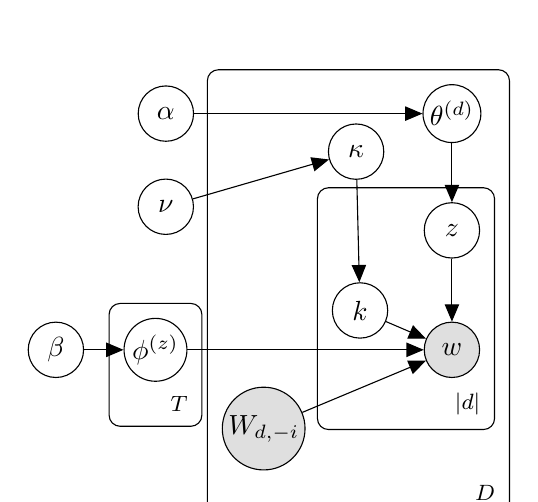
\begin{tikzpicture}[x=1.7cm,y=1.8cm]

  % Nodes

  \node[obs] (w)  {$w$} ;
  \node[latent, above=of w,above=0.8cm of w]    (z)      {$z$} ; %
  \node[latent, left=of w,left=0.45cm of w,yshift=0.5cm]    (k)      {$k$} ; %  
  \node[latent, above=of z,above=0.75cm of z]    (theta)  {$\theta^{(d)}$}; %
  \node[latent, left=of theta,left=2.9cm of theta] (atheta) {$\alpha$};
  \node[latent, left=of z,left=0.5cm of z,yshift=1cm]    (K)  {$\kappa$}; 
  \node[latent, left=of K,left=1.7cm of K,yshift=-0.7cm] (p) {$\nu$};
  
  % More nodes
  \node[latent, left=of w,left=3cm of w] (phi)  {$\phi^{(z)}$}; %
  \node[latent, left=of phi,left=0.5cm of phi]  (beta) {$\beta$}; %

  \node[obs, left=of w,left=1.5cm of w,yshift=-1cm] (r)  {$W_{d,-i}$}; %

%  \factor[above=of phi] {phi-f} {right:Dir} {} {} ; %

  \factoredge {p}  {p}     {K} ; %
  \factoredge {K}  {K}     {k} ; %
  \factoredge {k}  {k}     {w} ; %
  \factoredge {theta}  {theta}     {z} ; %
  \factoredge {atheta} {atheta} {theta} ; %

  \factoredge {phi}    {phi}     {w} ; %
  \factoredge {r}    {r}     {w} ; %
  \factoredge {beta}   {beta}   {phi} ; %
  \factoredge {z}   {z}   {w} ; %
 
  \plate[inner sep=5pt] {plate1} { %
    (k)
    (z)
    (w)%(w-gate) %
  } {$|d|$}; %
%  \plate[inner sep=5pt] {uttplate} {
%    (plate1)
%    (z)%(z-f)(z-f-caption) %
%  } {$U_d$}
  \plate[inner sep=5pt] {docplate} {
	(plate1)
	(K)
	(r)
	(theta)% (theta-f)(theta-f-caption) %
  } {$D$} ; %

  \plate[inner sep=5pt] {} { %
    (phi)%(phi-f)(phi-f-caption) %
  } {$T$} ; %

%  \plate[inner sep=5pt] {} { %
%   (atheta)
%  } {$L$};

\end{tikzpicture}
%\endpgfgraphicnamed

%%% Local Variables: 
%%% mode: tex-pdf
%%% Tex-master: "example"
%%% End: 
}
}
\end{center}
\caption[Plate diagrams for LDA and $\kappa$LDA]{Plate diagrams illustrating the differences between LDA and our proposed model\label{fig5:plates}}
\end{figure}

This generative process is provided as pseudocode in Algorithm~\ref{alg5:kLDA}.  For comparison we also give the generative process psuedocode for standard LDA as Algorithm~\ref{alg5:LDA}.  Our notation in Algorithm~\ref{alg5:kLDA} for the cache distribution at a specific word $w_{d,i}$, $Cache(W_{d,-i},i)$, is intended to convey that when $k_{d,i}=1$, the generative distribution for $w_{d,i}$ depends only on the observed words in $d$.  We use the shorthand $W_{d,-i}$ to denote the sequence of words in $d$ without $w_{d,i}$, which is equivalent to the set difference: $\{w_{d,1},\ldots,w_{d,|d|}\} \setminus w_{d,i}$ 

Plate diagrams contrasting our model with the standard LDA model are provided in Figure~\ref{fig5:plates}.  Graphically, we can illustrate the dependence of the current word $w_{d,i}$ both on the broad topic context, via latent topic state $z_{d,i}$ as well a cache of observed words, which we denote as $W_{d,-i}$ (cf. Figure~\ref{subfig5:kldaPlates}).  Within this notation, observed variables are shaded, latent variables unshaded, and the quantity at the lower right portion of the plate indicated the number of i.i.d. instances of the set of variables contained within.

We do not specify whether the cache component contains of unigrams or higher order N-grams.  Neither do we need to specify the size of the cache or any decay properties given the position $i$ in the document.  Without loss of generality, we can subsequently show that the model as presented easily handles any such variations of the cache that depend only on the observed words.


\begin{algorithm}[H]  
\caption{LDA generative process\label{alg5:LDA}}
\begin{algorithmic}[1]
\FOR{topic $t \in \mathcal{T}$}
    \PRINT{$\phi^{(t)}\sim\mbox{Dirichlet}(\beta)$}
    \COMMENT{Draw topic distributions}
\ENDFOR                                                

\FORALL{$d\in\mathcal{D}$}
	\PRINT{$\theta^{(d)}\sim\mbox{Dirichlet}(\alpha)$}
    \COMMENT{Draw topic proportions}
    \FOR{ $w_{d,i}, 1 \le i \le |d|$}
        \PRINT{$z_{d,i}\sim\theta^{(d)}$}
		\COMMENT{Draw word topic state}
   	    \PRINT{$w_{d,i}\sim\phi^{(t=z_{d,i})}$}
   	    \COMMENT{Generate word from topic}
    \ENDFOR
\ENDFOR
\end{algorithmic}
\end{algorithm}


%First we need to present the generative story for our proposed models, from which we can enumerate the latent and observed variables and express the model likelihood over a set of spoken documents.
Given this procedure and the dependencies between variables, we can factor the joint probability of observed and latent variables as follows:
\begin{equation}
\begin{aligned}
P(W,Z,K,\Theta,\Phi|\alpha,\beta,\nu) = P(\Phi|\beta)\cdot  P(\Theta|\alpha)\cdot P(\kappa|\nu)\cdot P(W,Z,K|\Theta,\Phi,\kappa)& \label{eqn5:joint} \\
= P(\Phi|\beta)\cdot P(\Theta|\alpha) \cdot P(\kappa|\nu) \cdot P(Z|\Theta,\Phi) \cdot P(K|\kappa)\cdot P(W|Z,K)& 
\end{aligned}
\end{equation}
We use uppercase letters to denote sequences of the variables from  Algorithm~\ref{alg5:kLDA} and Figure~\ref{subfig5:kldaPlates}.  

Now that we can express this factorization of the joint distribution, what we are most interested in for this and other graphical models is an estimate of the posterior distribution of the latent variables given the observed data.  In our cases, we want to estimate the distribution of the various $(\phi^{(t)}, \theta^{(d)},\kappa^{(d)})$, that is the \textit{\textbf{topics}}, \textbf{\textit{document-specific topic mixtures}}, and \textbf{\textit{document-specific cache usage}}, using the observed word sequences.  Without a closed-form solution, we need to turn to \textit{approximate posterior inference}, and in particular we employ a Collapsed Gibbs Sampling approach.

\section{Collapsed Gibbs Sampler}
\label{sec:sampler}
As was outlined in Section~\ref{sec:postInf}, in order to obtain the necessary machinery for a Gibbs sampler, we must obtain the sampling distributions for our latent variables $Z$ and $K$ where the value of a single latent variable is conditioned on the current state of all other variables, observed and unobserved (Equations~\ref{eqn5:zsamp},\ref{eqn5:ksamp}).   Here we present a derivation of both sampling distributions, how the per-document cache operates within the sampling framework, and the bookkeeping required for a reasonable implementation.
\begin{align}
P(z_{d,i}|W,Z_{-i},K) \label{eqn5:zsamp}\\
P(k_{d,i}|W,Z,K_{-i}) \label{eqn5:ksamp}
\end{align}

First, we simplify the joint probability by \textit{collapsing} the priors - integrating over $\Phi$, $\Theta$, and $K$.  This is a common technique for latent variable models such as LDA.   We collapse the priors in each factor of the joint probability to transform $P(W,Z,K,\Theta.\Phi)$ from Equation \ref{eqn5:collapsed} to \ref{eqn5:collapsed2}: 
\begin{align}
\begin{split}
P(W,Z,K,\Theta,\Phi|\alpha,\beta,\nu)
&=  \\
P(\Phi|\beta) &\cdot P(\Theta|\alpha) \cdot P(\kappa|\nu) \cdot P(Z|\Theta,\Phi) \cdot P(K|\kappa)\cdot P(W|Z,K) 
\end{split} \label{eqn5:collapsed} \\
%\end{equation}
%\noindent to:
%\begin{align}
P(W,Z,K|\alpha,\beta,\nu) &= 
P(W|Z,K,\beta) \cdot P(Z|\alpha) \cdot P(K|\nu) \label{eqn5:collapsed2}
\end{align}

\noindent We integrate out the priors $\Phi$, $\Theta$, and $K$ in a straightforward fashion because of the Dirichlet-Multinomial and Beta-Bernoulli conjugacy and conditional independence assumptions.

The second step in the derivation is to obtain the sampling distributions from this collapsed joint distribution.  It follows that:
\begin{align}
P(z_{d_0,j}=t_0|W,Z_{-j},K,\alpha,\beta,\nu) &= \frac{P(W,Z,K|\alpha,\beta,\nu)}{P(W,Z_{-j},K|\alpha,\beta,\nu)} \label{eqn5:zsampler} \\
P(k_{d_0,j,i}=k_0\in\{0,1\}|W,Z,K_{-i},\alpha,\beta,\nu) &= \frac{P(W,Z,K|\alpha,\beta,\nu)}{P(W,Z,K_{-i}|\alpha,\beta,\nu)} \label{eqn5:ksampler}
\end{align}
\noindent The numerator and denominator both refer to the closed form of the collapsed joint distribution, evaluated at particular choices for $W$, $Z$, and $K$ - \textit{the current sampling state plus the new possible values $t_0$ and $k_0$}.  The only difference is that the denominator does not contain terms for the state to be sampled.  

We have modeled our subsequent derivations after a very useful tutorial on Gibbs sampling by Korsos and Taddy (cf. \cite{korsos2011gibbs}).  They follow the usage from Steyvers et al. where topics are represented by $\Phi$, states by $Z$, per-document topic priors by $\Theta$ and hyperparameters $\alpha$ and $\beta$.   Keeping with this notation, we now show how to obtain the collapsed form for each factor of the joint probability (Equation~\ref{eqn5:collapsed}).  

\subsection{Notation}
To make the derivations of each factor readable, we introduce a handful of count vectors and other shorthand notations.  First, we use the term $I(\cdot)$ as an indicator function that returns 1 when its arguments are true and 0 otherwise.  Secondly, we use the notation $B(a)$ for both the Dirichlet and Beta $pdf$ normalizing factor given that the latter is a two-parameter instance of the generalized Beta function (cf. Eqn.~\ref{betaF}).
\begin{align}
B(a) &= \frac{\prod_{i=1}^{|a|}\Gamma(a_i)}{\Gamma(\sum_{i=1}^{|a|}a_i)} \label{betaF}
\end{align}
\noindent Count vectors that capture the current sampler state can be defined in terms of sums over indicator functions.

Each topic state variable $z_{d,i}\in Z$ is associated with a particular word $w_{d,i}=w_0$ and has an assigned state value corresponding to some topic $t_0$ - when the corresponding cache indicator $k_{d,i}=0$.  We aggregate the counts of states associated with a topic $t_0$ as vectors $C^{(t_0)}$ in the dimension of the vocabulary.  Subscripted by a particular word we can express the current topic-word association as:
\begin{equation}
	C^{(t_0)}_{w_0} = \sum_{d=1}^D \sum_{i=1}^{|d|} I(w_{d,i}=w_0 \land k_{d,i}=0 \land z_{d,i}=t_0)
\end{equation}
\noindent We also need to capture the current per-document topic mixture which we express by the $\mathcal{T}$-dimensional vector $N^{(d)}$, which is given by:
\begin{equation}
	N^{(d_0)}_{t_0} = \sum_{i=1}^{|d_0|} I(k_{d_0,i}=0 \land z_{d_0,i}=t_0)
\end{equation}

Each cache state variable $k_{d,i}\in K$, although also associated with a particular word $w_{d,i}=w_0$, as we will see, need only contribute to a document-level count. We define two vector terms $L$ and $T$ to capture the number of cache versus topic states in a particular document.
\begin{align}
	L_d &= \sum_{i=1}^{|d|} I(k_{d,i}=1) \\
	T_d &= \sum_{i=1}^{|d|} I(k_{d,i}=0) \\
	 \left[ \sum_{d=1}^D T_d\right]&= \sum_{t=1}^{\mathcal{T}} \sum_{v=1}^V C^{(t)}_{v}
\end{align}

As we only consider topic-word associations where the word is generated from a topic-state, the $K$ variables divides the corpus into two parts, words generated from the topics or words generated from the cache.  We necessarily have:
\begin{equation}
	\sum_{d=1}^D |d| = \left[\sum_{d=1}^D T_d\right] + \left[\sum_{d=1}^D L_d\right]
\end{equation}

From this, we can also describe our generative model for words by a process whereby a document author (or speaker) introduces some topical word, but then as he or she proceeds, based on a propensity for repetition ($\kappa^{(d)}$), repeats previously uttered words for either syntax or purposes of redundancy.  % does our analysis of individual words bear this out?
% HERE
\subsection{Derivations}
For the term $P(W|Z,K,\beta,\nu)$ we  integrate over the topic prior $\phi$.  The first observation we make is that the cached words do not depend at all on $\phi$, given the current cache state, so we can treat the cache probabilities independent of the topic likelihoods.

{\small
\begin{align}
P(W&|Z,K,\beta) \\
 &= \int_{\phi} P(W|Z,K,\phi)\cdot P(\phi|\beta) d\phi\\
 &= P_C(W_{\{k_{d,i}=1\}}) \int_{\phi} \left [ \prod_{t=1}^T \prod_{d=1}^D \prod_{i=1}^{|d|} P(w_i|z_{d,i}=t)^{I(k_{d,i}=0)}  \right ] P(\phi|\beta)\, d\phi \\
&= P_C(W_{\{k_{d,i}=1\}}) \int_{\phi} \left [ \prod_{t=1}^T \prod_{d=1}^D \prod_{i=1}^{|d|} {\phi_{w_i}^{(t)}}^{I(k_{d,i}=0)}  \right ]  \left [ \prod_{t=1}^T \frac{1}{B(\beta)} \prod_{v=1}^V {\phi_v^{(t)}}^{\beta_v-1} \right ]  d\phi\\
&= P_C(W_{\{k_{d,i}=1\}}) \int_{\phi} \prod_{t=1}^T \left [ \frac{1}{B(\beta)} \prod_{v=1}^V {\phi_v^{(t)}}^{\beta_v + C^{(t)}_v - 1} \right ]  d\phi\\
&= P_C(W_{\{k_{d,i}=1\}}) \prod_{t=1}^T \left [ \frac{B(\beta + C^{(t)})}{B(\beta)} \right ] 
\end{align}
}

We have denoted the cache probability of the sub-sequence of words whose cache state $k_{d,i}$ is currently set to 1 as $P_C(W_{\{k_{d,i}=1\}})$.  Expanding out this term, we obtain:
\begin{equation}
P_C(W_{\{k_{d,i}=1\}})=\prod_{d=1}^D \prod_{i=1}^{|d|} P_{cache}(w_{d,i}|W_{d,-i})^{I(k_{d,i}=1)}
\end{equation}
\noindent As we stated previously, we have shown our sampler can be constructed independently of the size, order, or any other properties of the cache language model.

Moving on, to  the term $P(K|\nu)$, we integrate out $\kappa$ by means of the Beta-Bernoulli conjugate prior in a manner identical to the Dirichlet-Multinomial prior.

\begin{align}
P(K|\nu) &= \int_{\kappa} P(K|\kappa)\cdot P(\kappa|\nu) d\nu\\
 &= \int_{\kappa} \prod_{d=1}^D  \left [ {\kappa^{(d)}}^{L_d} (1-\kappa^{(d)})^{T_d} \right] \left [ \frac{{\kappa^{(d)}}^{\nu_0} (1-\kappa^{(d)})^{\nu_1}}{B(\nu_0,\nu_1)} \right] d\kappa \\
 &= \int_{\kappa} \prod_{d=1}^D  \left [ \frac{{\kappa^{(d)}}^{\nu_0+L_d} (1-\kappa^{(d)})^{\nu_1+T_d}}{B(\nu_0,\nu_1)} \right] d\kappa \\
 &= \prod_{d=1}^D  \left [ \frac{B(\nu_0+L_d,\nu_1+T_d)}{B(\nu_0,\nu_1)} \right] 
\end{align}
 
 
The third term $P(Z|\alpha)$ can be obtained in the same manner by integrating over the topic mixtures $\theta$.  This quantity is derived in the same manner as a collapsed Gibbs sampler for standard LDA, except the topic counts must exclude words generated from cache states.
  
\begin{align}
 P(Z|\alpha) &= \int_{\theta} P(Z|\theta)\cdot P(\theta|\alpha) d\theta \\
  &= \int_{\theta} \prod_{d=1}^{D} \left [ \prod_{i=1}^{|d|} P(z_{d,i}|\theta^{(d)})^{I(z_{d,i}=0)} \right ] P(\theta_d|\alpha) d\theta \\
  &= \int_{\theta} \prod_{d=1}^{D} \left [ \prod_{i=1}^{|d|} {\theta^{(d)}_{z_{d,i}}}^{I(z_{d,i}=0)} \right ]\frac{1}{B(\alpha)} \prod_{t=1}^T {\theta^{(d)}_t}^{\alpha_t - 1}  d\theta \\
  &= \int_{\theta} \prod_{d=1}^{D} \left [ \frac{1}{B(\alpha)} \prod_{t=1}^T {\theta^{(d)}_t}^{\alpha_t + N^{(d)}_{t} - 1}  \right ] d\theta \\
  &= \prod_{d=1}^{D} \left [ \frac{B(\alpha + N^{(d)})}{B(\alpha)}  \right ] \label{zalpha}
\end{align}
 

Combining the closed form for the terms $P(W|Z,K,\beta)$, $P(K|\nu)$, and $ P(Z|\alpha)$ we obtain the desired joint probability $P(W,Z,K|\alpha,\beta,\nu)$:

\begin{equation}
P_C(W_{\{k_{d,i}=1\}}) \prod_{k=1}^T \left [ \frac{B(\beta + C^{(k)})}{B(\beta)} \right ] \prod_{d=1}^D  \left [ \frac{B(\nu_0+L_d,\nu_1+T_d)}{B(\nu_0,\nu_1)} \right ] \prod_{d=1}^{D} \left [ \frac{B(\alpha +  N^{(d)})}{B(\alpha)}  \right ] 
\end{equation}

\subsection{Sampling Distributions}
We can now use this collapsed, factored, joint probability to obtain the sampling distributions needed to update each topic state $z_{d,i}$ and cache state $k_{d,i}$.  For $Z$ we compute the sampling distribution for each possible topic value, iterating over each state, giving $\mathcal{T}\cdot|W|$ computations per iteration over the training corpus.   For $K$, which can take on values $\{0,1\}$, we have 2$\cdot|W|$ computations per iteration, so the overall sampling cost is still linear in the size of the corpus.

The key insight, which has been demonstrated numerous times in derivations for  LDA and similar variants, is that most terms in the joint probability are unchanged when considering different values for a particular state $z_{d,i}$.  Removing the particular state $z_{d_0,j}$ from the sequence only changes the count vectors $C^{(t_0)}$ and $N^{(d_0)}$ for one topic in one dimension ($v=w_{d_0,j})$.  All other $B(\cdot)$ terms in other documents for other topics cancel.  Also, because we are sampling a topic state, we must assume the cache variable $k_{d_0,j}=0$.  This implies that sub-sequences $W_{\{k_{d_0,i}=1\}}$ and $W_{\{k_{d_0,i}=1\},-j}$ are identical, so the cache probabilities cancel as well.

\begin{align}
P(z_{d_0,j}&=t_0|W,Z_{-j},K,\alpha,\beta,\nu) = \frac{P(W,Z,K|\alpha,\beta,\nu)}{P(W,Z_{-j},K|\alpha,\beta,\nu)} \label{zsampler3} \\
&= \frac{P(Z|\alpha) \cdot P(W|Z,K,\beta) \cdot P(K|\nu)}{P(Z_{-j}|\alpha) \cdot P(W|Z_{-j},K,\beta) \cdot P(K|\nu)}  \\
&= \frac{P(Z|\alpha)\cdot P(W|Z,K,\beta)}{P(Z_{-j}|\alpha) \cdot P(W_{-j}|Z_{-j},K,\beta) \cdot P(W_j|\alpha,\beta)} \\
&\propto \frac{P(Z|\alpha)\cdot P(W|Z,K,\beta)}{P(Z_{-j}|\alpha) \cdot P(W_{-j}|Z_{-j},K_{-j},\beta)} \label{samplerUnnorm2} \\
&\propto \prod_{d=1}^{D} \left [ \frac{B(\alpha +  N^{(d)})}{B(\alpha +  N^{(d)}_{-j}) } \right ] \cdot \frac{P(W_{k=1})}{P(W_{-j,k=1}) } \cdot \prod_{t=1}^T \left [ \frac{B(\beta + C^{(t)})}{B(\beta + C^{(t)}_{-j}) } \right ]  \\
&\propto \frac{B(\alpha +  N^{(d_0)})}{B(\alpha +  N^{(d_0)}_{-j})} \cdot \frac{B(\beta + C^{(t_0)})}{B(\beta + C^{(t_0)}_{-j})}
\end{align}

% assumptions P(W|K...)

Applying the definition of the $B(\cdot)$ function (from the Dirichlet distributions of $\Phi$ and $\Theta$), we can further simplify the various $\Gamma(\cdot)$ expressions.  For brevity, we'll express the components of vector arguments $[\alpha + N^{(d)}]_t$ and $[\beta + C^{(t)}]_v$ as $a_t$ and $c_v$ respectively.

\begin{align}
P(z_{d_0,j}&=t_0|W,Z_{-j},K,\alpha,\beta,\nu) \label{zsampImpl} \\
&\propto \frac{B\left(\alpha +  N^{(d_0)}\right) \cdot B\left(\beta + C^{(t_0)}\right) }{ B\left(\alpha +  N^{(d_0)}_{-i}\right) \cdot B\left(\beta + C^{(t_0)}_{-i}\right)} \label{sampler2} \\
&\propto \frac{\prod_{t=1}^T \Gamma(a_t)}{\Gamma\left(\sum_{t=1}^T a_t \right)} \frac{\Gamma\left(-1+\sum_{t=1}^T a_t \right)}{\Gamma(a_{t_0}-1) \prod_{t\ne t_0} \Gamma(a_t)}
\frac{ B\left(\beta + C^{(t_0)}\right) }{ B\left(\beta + C^{(t_0)}_{-i}\right)}\\
&\propto \frac{\Gamma(a_{t_0})}{\left(\sum_{t=1}^T a_t \right)\Gamma(a_{t_0}-1)} \frac{ B\left(\beta + C^{(t_0)}\right) }{ B\left(\beta + C^{(t_0)}_{-i}\right)}\\
&\propto \frac{a_{t_0}}{\left(\sum_{t=1}^T a_t \right)} \frac{ B\left(\beta + C^{(t_0)}\right) }{ B\left(\beta + C^{(t_0)}_{-i}\right)} \\
&\propto \frac{a_{t_0}}{\left(\sum_{t=1}^T a_t \right)} \frac{\prod_{v=1}^V \Gamma(c_v)}{\Gamma\left(\sum_{v=1}^V c_v \right)} \frac{\Gamma\left(-1 + \sum_{v=1}^V c_v\right)}{\Gamma(c_{w_{d_0,j}}-1)\prod_{v\ne w_{d_0,j}} \Gamma(c_v)} \\
&\propto \frac{a_{t_0}}{\left(\sum_{t=1}^T a_t \right)} \frac{ \Gamma(c_{w_{d_0,j}})}{\left(\sum_{v=1}^V c_v \right)\Gamma(c_{w_{d_0,j}}-1)} \\
&\propto \frac{a_{t_0}}{\left(\sum_{t=1}^T a_t \right)} \frac{ c_{w_{d_0,j}}}{\left(\sum_{v=1}^V c_v \right)} \\
&\propto \frac{(\alpha_{t_0}+N^{(d_0)}_{t_0})}{\left(\sum_{t=1}^T \alpha_{t}+N^{(d_0)}_{t_0} \right)} \frac{(\beta +C^{(t_0)}_{w_j})}{\left(\sum_{v=1}^V \beta+C^{(t_0)}_{v} \right)} \label{eqn5:zsampImpl}
\end{align}
%P(z_i=k_0|W,Z_{-i},\alpha,\beta)

Evaluating Equation~\ref{eqn5:zsampImpl} for each possible topic value $t_0$ gives a proportional set of values that can be used to sample from $P(z_{d,i})$ for each topic state.  In terms of notation, this looks exactly like LDA, except the term-topic counts must not contain words in the sampler state currently drawn from the cache.

%This final equation can be used directly to build a Gibbs sampler for our new model, maintaining the counts $N^{(d)}$ and $C^{(t)}$.  
For the cache states, we can take a number of simplifying assumptions.  First, if a word $w_{d_0,j}$ is going to be drawn from the cache state ($k_{d_0,j}=1)$ then the topic count vectors $C^{(t)}$ and $C^{(t)}_{-j}$, with and without state $k_{d_0,j}$ are identical, so the $\beta$ terms drop out. Also, the number of topic states is unchanged ($T_d$) and the number of cache states differs only for document $d_0$.   Assuming conditional of the word probabilities from the cache, as one might expect, the sample probability of the cache state depends only on the cache probability of the word in $d_0$ at position $j$ (cf. Equation~\ref{ksampler3}).
\begin{align}
P(k_{d_0,j}&=1|W,Z,K_{-j},\alpha,\beta,\nu) = \frac{P(W,Z,K|\alpha,\beta,\nu)}{P(W,Z,K_{-j}|\alpha,\beta,\nu)} \\
&\propto \frac{P_C(W_{\{k_{d_0,i}=1\}})}{P_C(W_{-j,\{k_{d_0,i}=1\}}) } \cdot \prod_{t=1}^T \left [ \frac{B(\beta + C^{(t)})}{B(\beta + C^{(t)}_{-j}) } \right ] \cdot \prod_{d=1}^{D} \left [ \frac{B(\nu_0+L_d,\nu_1+T_d)}{B(\nu_0+(L_d)_{-j},\nu_1+ (T_d)_{-j}} \right ]  \\
&\propto P_C(w_{d_0,j}|W_{d,-j})\cdot \frac{B(\nu_0+L_{d_0},\nu_1+T_{d_0})}{B(\nu_0+L_{d_0} - 1,\nu_1+T_{d_0})}  \label{ksampler3}
\end{align}

However, if a word at ${(d_0,j)}$ is to be drawn from a topic instead (Eqn.~\ref{ksampler2}), the number of cache states ($L_d$) is unchanged for all documents so the cached word sequences $W_{\{k_{d,i}=1\}}$ and $W_{-j,\{k_d,i\}=1}$ are identical, and that term can be removed.  

\begin{align}
P(k_{d_0,j}&=0|W,Z,K_{-j},\alpha,\beta,\nu) = \frac{P(W,Z,K|\alpha,\beta,\nu)}{P(W,Z,K_{-j}|\alpha,\beta,\nu)} \label{ksampler2} \\
&= \frac{P(Z|\alpha) \cdot P(W|Z,K,\beta) \cdot P(K|\nu)}{P(Z|\alpha) \cdot P(W|Z,K_{-j},\beta) \cdot P(K_{-j}|\nu)}  \\
&= \frac{P(W|Z,K,\beta)\cdot P(K|\nu)}{P(W_{-j}|Z,K_{-j},\beta) \cdot P(K_{-j}|\nu) \cdot P(W_j|\alpha,\beta) } \\
&\propto \frac{P(W|Z,K,\beta)\cdot P(K|\nu)}{P(W_{-j}|Z,K_{-j},\beta) \cdot P(K_{-j}|\nu) } \label{ksamplerUnnorm2} \\
&\propto \frac{P_C(W_{\{k_{d_0,i}=1\}})}{P_C(W_{-j,\{k_{d_0,i}=1\}}) } \cdot \prod_{t=1}^T \left [ \frac{B(\beta + C^{(t)})}{B(\beta + C^{(t)}_{-j}) } \right ] \cdot \prod_{d=1}^{D} \left [ \frac{B(\nu_0+L_d,\nu_1+T_d)}{B(\nu_0+L_d,\nu_1+ (T_d)_{-j}} \right ]  \\
&\propto \frac{B(\beta + C^{(z_j)})}{B(\beta + C^{(z_j)}_{-j})} \cdot \frac{B(\nu_0+L_{d_0},\nu_1+T_{d_0})}{B(\nu_0+L_{d_0},\nu_1+T_{d_0} - 1)} 
\end{align}


As with the sampling distribution for $Z$, we can expand the $B(\cdot)$ function and simplify to obtain a closed form for the $K$ sampling distribution values.  Given that the Beta distribution normalizer is a two-parameter case of the generalized $B(\cdot)$ normalizer for the Dirichlet, we get the same simplification result as in Equation~\ref{zsampImpl}.

\begin{align}
P(k_{d_0,j}&=1|W,Z,K_{-j},\alpha,\beta,\nu)  \\
& \propto P_C(w_{d_0,j}|W_{d,-j})\cdot \frac{B(\nu_0+L_{d_0},\nu_1+T_{d_0})}{B(\nu_0+L_{d_0} - 1,\nu_1+T_{d_0})} \\
& \propto P_C(w_{d_0,j}|W_{d,-j})\cdot\frac{\nu_0 + L_{d_0}}{(\nu_0+\nu_1 + |d_0|)}
\end{align}

\begin{align}
P(k_{d_0,j}&=0|W,Z,K_{-j},\alpha,\beta,\nu)  \\
&\propto \frac{B(\beta + C^{(z_j)})}{B(\beta + C^{(z_j)}_{-j})} \cdot \frac{B(\nu_0+L_{d_0},\nu_1+T_{d_0})}{B(\nu_0+L_{d_0},\nu_1+T_{d_0} - 1)}  \\
& \propto 
\frac{(\beta +C^{(t_0)}_{w_j})}{\left(\sum_{v=1}^V \beta+C^{(t_0)}_{v} \right)} \frac{\nu_1 + T_{d_0}}{(\nu_0+\nu_1 + |d_0|)} \label{ks01}\\
& \propto 
\frac{\nu_1 + T_{d_0}}{(\nu_0+\nu_1 + |d_0|)} \label{ks02}
\end{align}

As the sampler depends on the prior state of $Z$, which is captured in the count vectors $C^{(t)}$.  If the previous state of $k_{d_0,j}$ were 0, then  $z_{j}$ will have some topic state $t_0$, so the probability mass is proportional to Equation ~\ref{ks01}.  However, if the previous state of $k_{d_0,j}$ were 1, a cache state, then we would argue that the count vectors  $C^{\cdot}$ and $C^{\cdot}_{-j}$ are identical, so mass can be simplified to Equation ~\ref{ks02}.  Other assumptions here for implementation are certainly possible.   A pseudocode example for the sampler is provided in Appendix~\ref{sec:pseudocode}.

\subsection{Summary}

In brief, we've derived the quantities necessary to estimate all the parameters of our proposed model using a Gibbs Sampling procedure.   
\begin{align}
P(z_{d_0,j}=t_0|W,Z_{-j},K,\alpha,\beta,\nu) &\propto \frac{(\alpha_{t_0}+N^{(d_0)}_{t_0})}{\left(\sum_{t=1}^T \alpha_{t}+N^{(d_0)}_{t_0} \right)} \frac{(\beta +C^{(t_0)}_{w_j})}{\left(\sum_{v=1}^V \beta+C^{(t_0)}_{v} \right)} \label{eqn5:zsampFinal} \\
P(k_{d_0,j}=1|W,Z,K_{-j},\alpha,\beta,\nu) &\propto P_C(w_{d_0,j}|W_{d,-j})\cdot\frac{\nu_0 + L_{d_0}}{(\nu_0+\nu_1 + |d_0|)} \label{eqn5:ksampImpl}\\
P(k_{d_0,j}=0|W,Z,K_{-j},\alpha,\beta,\nu) &\propto 
\frac{(\beta +C^{(t_0)}_{w_j})}{\left(\sum_{v=1}^V \beta+C^{(t_0)}_{v} \right)} \frac{\nu_1 + T_{d_0}}{(\nu_0+\nu_1 + |d_0|)}  
\end{align}

At any point in the sampling procedure we can then obtain quantities for the topics, $\phi$, topic mixtures $\theta$, and cache usage $\kappa$ as:
\begin{align}
[\phi^{(t)}]_{w} = \frac{\beta_w + C^{(t)}_{w}}{\sum_{v=1}^V \beta_v + C^{(t)}_v} \\
[\theta^{(d)}]_{t_0} = \frac{\alpha_{t_0} + N^{(d)}_{t_0}}{\sum_{t=1}^\mathcal{T} \alpha_t + N^{(d)}_t} \\
\kappa^{(d)} = \frac{\nu_0 + L_d}{\nu_0 + \nu_1 + |d|} 
\end{align}

\section{N-gram Extension}
Given this framework, it is straightforward (and has been shown elsewhere) to extend the LDA Gibbs sampling algorithm to N-grams (cf. \cite{wang2007topical}). The Topical N-gram model of Wang et al. allows for conditional formation of N-grams.  An alternative approach would be to allow every word drawn from a topic distribution to also be conditioned on the preceding $(N-1)$ words.

%To arrive at the sampler we only need re-derive $P(W|Z,\beta)$ with this assumption.  
Without any additional constraints, each topic $\phi$ can now be expressed as a set of multinomial distributions, one for each possible (N-1) length word history.   The unigram parameter $[\phi^{(t)}]_w$ becomes $[\phi^{(h,t)}]_w$, which captures the probability of word $v$, conditioned on the word history $h$ and given topic $t$, $P(w|h,t)$.  As $\phi$ arises only in the sampling distribution for topic states $z_{d,i}$, it turns out we only need a slight modification to the unigram $Z$ sampler (Equation~\ref{eqn5:zsampFinal}).  We only need to recompute the sub-term $P(W|Z,K,\beta)$.   

First, as before, we integrate out the $\phi$ terms (Eqn.~\ref{eqn5:ngram1}).  Although all $\mathcal{T}\cdot V^{N-1}$ distributions appear in $P(W|Z,K,\beta)$ when we compute the sampling distribution, only the terms for the current topic and word history remain (cf. Equation~\ref{eqn5:ngram2}).
\begin{align}
P(W&|Z,K,\beta) \\
 &= \int_{\phi} P(W|Z,K,\phi)\cdot P(\phi|\beta) d\phi\\
 &= P_C(W_{\{k_{d,i}=1\}}) \int_{\phi} \left [ \prod_{t=1}^T \prod_{d=1}^D \prod_{i=1}^{|d|} P(w_i|h_i,z_{d,i}=t)^{I(k_{d,i}=0)}  \right ] P(\phi|\beta)\, d\phi \\
&= P_C(W_{\{k_{d,i}=1\}}) \int_{\phi} \left [ \prod_{t=1}^T \prod_{d=1}^D \prod_{i=1}^{|d|} {\phi_{w_i}^{(h_i,t)}}^{I(k_{d,i}=0)}  \right ]  \left [ \prod_{t=1}^T \prod_{h=1}^{V^{N-1}} \frac{1}{B(\beta^{(h)})} \prod_{v=1}^V {\phi_v^{(h,t)}}^{\beta^{(h)}_v-1} \right ]  d\phi\\
&= P_C(W_{\{k_{d,i}=1\}}) \int_{\phi} \prod_{t=1}^T \left [ \prod_{h=1}^{V^{N-1}} \frac{1}{B(\beta^{(h)})} \prod_{v=1}^V {\phi_v^{(h,t)}}^{\beta_v + C^{(t)}_v - 1} \right ]  d\phi\\
&= P_C(W_{\{k_{d,i}=1\}}) \prod_{t=1}^T \left [\prod_{h=1}^{V^{N-1}} \frac{B(\beta^{(h)} + C^{(h,t)})}{B(\beta^{(h)})} \right ] \label{eqn5:ngram1}
\end{align}


As with the topics $\phi$, we also index the counts for topics and words by word histories $h$. The counts $C^{(t)}$ from the unigram case become $C^{(h,t)}$, where $[C^{(h,t)}]_w$ is the number of occurrences of $w$ with history $h$ and with topic state $t$.  Because, as with the unigram case, during sampling these count vectors only differ by 1 at any particular word, the $P(W|Z,K,\beta)$ term of the sampling proportions can now be expressed as:

\begin{align}
\frac{P(W|Z,K,\beta)}{P(W_{-j}|Z_{-j},K,\beta)} &= \prod_{h=1}^{V^{n-1}} \left [ \frac{B(\beta^{(h)} + C^{(h,t)})}{B(\beta^{(h)} + C^{(h,t)}_{-1})} \right ] \label{eqn5:ngram2} \\
&= \frac{B(\beta^{(h_0)} + C^{(h_0,t)})}{B(\beta^{(h_0)} + C^{(h_0,t)}_{-j})} \\
&= \frac{\beta^{(h_0)} + C^{(h_0,t)}_{w_{d,j}}}{\sum_{h=1}^{V^{N-1}} \beta^{(h)} + C^{(h,t)}_{w_{d,j}}} \label{eqn5:ngram3}
\end{align}

%This quantity can be applied to the sampling distributions from 
\section{Conclusion}
We have fully described a latent topic model framework the jointly models words as either generated from a broad context (topics) or local context (cache).   We have also derived the computations necessary to perform parameter estimation, by means of approximate posterior inference, using a Gibbs sampler.  Our model can accommodate any type of document-level cache model that conditions the probability of a particular word only on other observed words in the same document.

Two main questions we will address in the remaining chapters.   First, how well does this model capture both topic repetition properties of the data?   Secondly, returning to our motivating problem, does this model generate useful language models for speech retrieval?


\begin{figure}[t]
\begin{center}
\scalebox{1.2}{\input{model_clda_ngram}}
\end{center}
\caption[Ngram $\kappa$LDA]{N-gram Cache-augmented Topic Model}
\end{figure}


\chapter{Model Analysis}
\label{sec:kldaAnalysis}

Any proposed model such as the one detailed in Chapter~\ref{sec:klda} can be analyzed either \textit{intrinsically} or \textit{extrinsically}, with or without reference to a particular task.   We evaluated standard LDA and cache-based language models extrinsically in Chapter 4 in the context of the keyword retrieval task, and we will evaluate our proposed cache-augmented topic model on the same extrinsic task in Chapter 7.  In this chapter, we begin by looking directly at intrinsic, observable properties of the model, but also examine model properties through extrinsic tasks such as language modeling and topic discovery.

%We devote this chapter to an intrinsic analysis of our proposed model.  
We estimate model parameters on informal speech corpora in a number of languages and consider the model behavior from different perspectives.  We first look at the convergence and consistence of the approximate inference process itself.  Given the stochastic nature of Gibbs sampling, we look at consistency and convergence across multiple iterations on the same corpora.  Next we look specifically of the repetition properties inferred by our model.  We ask whether the inferred cache properties correspond to our intuitions and related repetition phenomena of the data.   We then look at constructing a unigram language model from the learned topic distributions and look at perplexity behavior on held out data, contrasting this with standard LDA models on the same data.  Lastly, we use external topic discovery tasks to asses the quality of the `subject matter' topic distributions.

% as with the work on repetition, we want kappa to reflect repetition quantity of the corpus, but also want that to be useful for the interpolation task

\section{Convergence and Consistency}

In recent years, many approximate inference techniques have been well studied in the context of the standard LDA topic model, to include different implementations and optimizations (cf. \cite{hoffman2010online}, \cite{zhai2012mr}, \cite{yao2009efficient}).  One standard point of comparison is the \textit{convergence} of different algorithms or models in terms of some metric.  Convergence speaks to both the stability of the model and the efficiency of inference algorithm.  Typically convergence can be expressed as the \textit{likelihood} (or derived metrics, \textit{log-likelihood} or \textit{perplexity}) of either the training data or a held out data set under the model.

Additionally, because of the stochastic nature of Gibbs Sampling (and other MCMC) approaches we can ask how \textit{consistent} different runs of the inference algorithm are for LDA or for our cache-augmented model.  To illustrate  both consistency and convergence of our proposed model, we perform 5 trials of parameter estimation on a number of similarly sized speech corpora.  We can show that in terms of consistency, both LDA and our cache-augmented model are equivalently stable across trials and exhibit similar convergence behavior over time.  We also analyze the convergence and consistency specifically of the $\kappa^{(d)}$ parameter under different corpora and number of topics.  Again, we can show the parameter estimation converges and is stable across trials, but as intuition suggests, the behavior differs across languages.

In this chapter and in the next we focus primarily on low-resource speech recognition and retrieval scenarios.  As before we utilize Limited Language Pack (Limited LP) resources from the IARPA {\small Babel} program, which contain only 10 hours of transcribed audio.  The languages we consider in this chapter include Turkish, Tagalog, Vietnamese, Zulu and Tamil.\footnote{Language collection releases babel105b-v0.4, babel106-v0.2g, babel107b-v0.7, babel206b-v0.1e, and babel204b-v1.1b respectively.}  
% NOTE and for task evaluation which require labels, we use spanish and enlgish
For interpretability of topics and cached words, we also estimate models on the CallHome Spanish corpus from LDC, which contains roughly 14 hours of transcribed conversational speech \cite{callhome}, LDC's Fisher Spanish transcripts \cite{ldc2010}, with 178 hours of transcribed speech, and the 359 hour subset of LDC's Fisher English transcripts we previously used for Topic ID experiments.

\begin{table}[t]
\begin{center}
   \begin{tabular}{lrrrr}\toprule
   \textbf{Corpus}  &  \textbf{Docs} & \textbf{Utts/Doc} & \textbf{Tokens/Doc} & \textbf{Tokens/Utt}\\ \midrule
   Turkish & 128 & 81.45 & 565.17 & 6.94 \\
   \rowcolor{blue!5} Tagalog & 132 & 87.52 & 534.02 & 6.10 \\
   Vietnamese & 126 & 80.71 & 932.86 & 11.56 \\
   \rowcolor{blue!5}   Zulu & 124 & 85.20 & 520.45 & 6.12 \\
   Tamil & 125 & 85.77 & 601.57 & 7.01 \\
   \rowcolor{blue!5}   Spanish (CallHome) & 160 & 107.51 & 903.84 & 8.41	\\
   Spanish (Fisher) & 1286 & 159.25 & 986.32 & 6.19 \\
   \rowcolor{blue!5} English (Fisher) & 2060 & 189.31 & 1899.05 & 10.03 \\\bottomrule
  \end{tabular}
\caption[Corpus sizes, conversational speech]{Corpus sizes in terms of documents, utterances, and word tokens\label{fig6:cstats}}
\end{center}

\end{table}

Corpus statistics are provided in Table~\ref{fig6:cstats}.  The Babel corpora are roughly all of the same size in terms of number and length (number of utterances) of documents.  For speech corpora, we generally use silence-segmented utterances, roughly corresponding to a single conversation turn, instead of sentences.  Sentences are generally not well delineated in speech transcripts.  The Spanish corpora contain noticeably longer documents at least in terms of the number of utterances.  English contains more words per utterance.  There is some variance in terms of the number of word tokens per utterance, particularly for Vietnamese, which as has been mentioned was transcribed with syllable level word tokens.  %This, as opposed to document length we might expect to be more a language-specific property.
%Likelihood  LDA (1, 2 gram) vs kLDA

\begin{figure}
\begin{center}
\includegraphics[width=0.5\textwidth]{graphs/ch6/ll/chsp-lda-ll.png}
\end{center}
\caption[Log-likelihood convergence, CallHome Spanish]{Model log-likelihood convergence over sampling process for CallHome Spanish transcripts.\label{fig6:llCallHome}}
\end{figure}

For each corpus we analyze the training log-likelihood (per word token) over 1000 iterations of Gibbs Sampling, and averaged over 5 independent trials.  We contrast the Mallet implementation of LDA with our proposed cache-augmented model (abbreviated $\kappa$LDA) with either unigram or bigram cache.  We also consider topic mixtures (under all models) of \{50,100,150,200\}.  

Figure~\ref{fig6:llCallHome} illustrates the convergence of the per-word log-likelihood over 1000 iterations for each model condition when training on the CallHome Spanish corpus.  The shaded area around the 100 topic condition indicates $\pm$ 1 sample standard deviation of the log-likelihood measurement across the 5 trials.   The tightness of the log-likelihood estimates over all iterations indicates that sampling under our cache-augmented model is roughly as stable as LDA across trials.  

% generated by graphs/ch6/ll2.R

\begin{figure}
\begin{center}
\subfloat[Vietnamese\label{fig6:llVietnamese}]{%
\includegraphics[width=0.45\textwidth]{graphs/ch6/ll/vietnamese-lda-ll.png}
}
\hfill
\subfloat[Turkish\label{fig6:llTurkish}]{%
\includegraphics[width=0.45\textwidth]{graphs/ch6/ll/turkish-lda-ll.png}
}
\end{center}
\caption[Log-likelihood convergence, Babel Corpora]{Model log-likelihood convergence over sampling process for Babel Vietnamese and Turkish transcripts.\label{fig6:llComp}}
\end{figure}


For the sake of comparison we present the convergence figures for the Babel Vietnamese and Turkish (cf. Figures~\ref{fig6:llVietnamese},~\ref{fig6:llTurkish}).  Indeed from a convergence perspective, the two behave similarly under standard LDA.  However the sampling becomes significantly less smooth moving from Vietnamese to Turkish.  For completeness, we include convergence figures for all corpora in Appendix~\ref{sec:llconverge}.  With respect to log-likelihood convergence, in all cases the trajectory consistently changes around iteration 250, which is consistent with the application of the hyperparameter re-estimation from Wallach et al.\cite{wallach2009} from that point on in all trials.

Alternatively, if we look at the absolute model log-likelihood we see that the cache-augmented models underperform standard LDA in both the unigram and bigram cache cases.  However we will re-visit this shortly in terms of language model perplexity.  Table~\ref{fig6:llstats} details the likelihood values as well as the sample standard deviation across trials (in parentheses) under all model conditions.  Irrespective of the absolute value, the low variance across trials is a quantitative indication of the likelihood stability of both LDA and our proposed variants.  Included are the results for the 100 topic case, with results for the 50, 150, and 200 topic case provided in full in Appendix~\ref{sec:llconverge}.

\begin{table}[t]
\begin{center}
   \begin{tabular}{lrrr}\toprule
   \textbf{Corpus} & \textbf{LDA} & \textbf{$\kappa$LDA-1} & \textbf{$\kappa$LDA-2}\\ \midrule
Turkish &  -7.554 (0.02) & -9.173 (0.04) & -8.535 (0.02) \\
Tagalog &  -6.523 (0.02) & -8.210 (0.03) & -7.910 (0.04) \\
Vietnamese & -6.498 (0.01) & -8.245 (0.03) & -8.044 (0.03) \\
Zulu &  -7.887 (0.02) & -9.912 (0.03) & -8.594 (0.03) \\
Tamil &  -7.887 (0.02) & -9.993 (0.04) & -8.853 (0.03) \\
Spanish (CallHome) &  -7.034 (0.02) & -8.341 (0.04) & -8.164 (0.04) \\
Spanish (Fisher) & -7.505 (0.01) & -8.381 (0.01) & -8.270 (0.03) \\
 \bottomrule
  \end{tabular}
\caption[Model log-likelihood per word]{Model log-likelihood per word after 1000 iterations, averaged over 5 runs, sample standard deviation in parenthesis.\label{fig6:llstats}}
\end{center}
\end{table}


\section{Repetition}
\label{sec:kldaRepetition}

The next manner in which we can look intrinsically at the parameters output by our cache-augmented model is by analyzing to what extent the latent variables capture token \textit{repetition} within various corpora.  Within our model, repetition is captured by the cache indicator variables $k_{d,i}$ and per-document cache prior $\kappa^{(d)}$.  We expect the former to be assigned to word types that tend to repeat within documents and the latter to represent the amount of repetition within a particular document, and generally this is in fact the case when looking at the data.

We continue to analyze the corpora described in the previous section, however we focus primarily on the IARPA Babel corpora, which are designed to be of equal size both in terms of length and number of documents.  We will first look at estimates for the prior term $\kappa^{(d)}$ then look at individual state assignments $k_{d,i}$.  

One lens through which we view how our proposed model captures repetition is the corpus $\kappa$ value, defined as the mean over all documents' $\kappa^{(d)}$.  We expect this value to correspond to language-specific tendencies towards repetition similar to what we found in Chapter~\ref{sec:repetitionRetrieval} with our learned interpolation weight $\widehat{\alpha}$ for repeated keywords. 

As with likelihood, we also look at the convergence and stability of the estimates of $\kappa$ during the sampling process.  Unlike the likelihood, which we expect in general to only increase, we have no such expectation for the $\kappa$ estimates.  The convergence figures for Vietnamese and Turkish are shown in Figure~\ref{fig6:kldaKappaIt} and the same for all languages are given in Appendix~\ref{sec:llconverge}.   As with the log-likelihood across trials, the sample standard deviation for the mean of $\kappa^{(d)}$ across 5 trials was 0.01 or less for all languages and conditions, again letting us quantify the stability of the sampling procedure.

\begin{figure}
\begin{center}
\subfloat[Vietnamese\label{subfig6:kVietnamese}]{%
\includegraphics[width=0.45\textwidth]{graphs/ch6/vietnamese-kappa-iters.png}
}
\hfill
\subfloat[Turkish\label{subfig6:kTurkish}]{%
\includegraphics[width=0.45\textwidth]{graphs/ch6/turkish-kappa-iters.png}
}
\end{center}                    
\caption[Convergence and stability of corpus $\kappa$]{Convergence and stability in $\kappa$LDA sampling process for corpus $\kappa$. \label{fig6:kldaKappaIt}}
\end{figure}

We highlight Turkish and Vietnamese as two languages whose repetition behavior we would expect to be most distinct.  Morphologically the two languages are quite different.  Turkish is an agglutanitive language and also exhibits vowel harmony between roots and affixes.  The result of multiple affixes, plus their harmonized forms, applied to a root word results in a large number of distinct word types as compared to other corpora (see \cite{mengusoglu2001} for a discussion of the implications of these properties for speech recognition and language modeling). From our perspective, the addition of affixes may have the effect of turning a word token which could have been a repetition of a previous token into a new word type, lowering the likelihood of repetition.

Vietnamese, by contrast is transcribed at the syllable level and for speech recognition, N-gram language models are also applied at the syllable level, so for purposes of comparison the only available word unit is the syllable.  Although it is sometimes described as `devoid of morphology' \cite{noyer1998vietnamese} many of its units have what Noyer describes as a `reduplicative counterpart' in which the syllable is repeated, perhaps with a change in tone to serve different syntactic or semantic roles.  This, in addition to the combinatorics of a fixed alphabet and small word length limits the number of possible word types and thus increased the likelihood that any particular word type will be repeated in a particular document.

\begin{table}
\begin{center}
   \begin{tabular}{lcccc}
   \textbf{Language}  & $\mathbf{\mathcal{T}=50}$ & \textbf{100} & \textbf{150} & \textbf{200} \\ \midrule
     Tagalog &  0.41 & 0.29 & 0.22 & 0.16 \\
     \rowcolor{blue!5}  Turkish &  0.31 & 0.19 & 0.13 & 0.09 \\
     \rowcolor{blue!5}  Vietnamese & 0.51 & 0.39 & 0.29 & 0.22 \\
     Zulu & 0.33 & 0.26 & 0.21 & 0.16 \\
     Tamil &  0.36 & 0.27 & 0.18 & 0.14 \\ \bottomrule
        \end{tabular}
\caption[Corpus $\kappa$ inferred from development data]{Corpus $\kappa$ inferred from 10 hour development data, by number of latent topics\label{kappas}}
\end{center}
\end{table} 

Table~\ref{kappas} lists the corpus $\kappa$ values for the Babel development corpora, with Turkish and Vietnamese figures called out. Figure~\ref{fig6:devKappa} shows the same estimates, and include error bars representing 1 sample standard deviation across 5 independent trials.  As we would have expected, for a particular number of latent topics $\mathcal{T}$, the highest $\kappa$ value is inferred from the Vietnamese corpus, and the lowest, indicating least token repetition, is inferred from the Turkish Corpus.  

We compare our $\kappa$ estimates to a simple measure of repetition in each corpus, the percentage of tokens in each document that are repeated (i.e. non-singletons).  
\begin{equation}
Document\,Repetition=\frac{1}{|D|}\sum_{d\in D} \left[ 1-\frac{\text{\# types in }d}{\text{\# tokens in }d}\right]
\end{equation}This better quantifies our intuition about the repetition within the Babel languages, as Zulu, Tamil, and Turkish have both low within-document token repetition and low corpus $\kappa$, while Vietnamese has both high $\kappa$ and a high percentage of token repetition (cf. Figure~\ref{fig6:docRep}).
\begin{figure}
\begin{center}
\includegraphics[width=0.7\textwidth]{graphs/ch6/kappas-dev.png}
\end{center}
\caption[Corpus $\kappa$ inferred from development corpora]{Corpus $\kappa$ inferred from development corpora, averaged over 5 sampling runs.\label{fig6:devKappa}}
\end{figure}
\begin{figure}
\begin{center}
\includegraphics[width=0.7\textwidth]{graphs/ch6/docRep.png}
\end{center}
\caption[Corpus $\kappa$ and per-document token repetition]{Corpus $\kappa$ of development corpora, compared against the percentage of repeated tokens within each document. \label{fig6:docRep}}
\end{figure}

% 
% cd graphs/ch6
% source('corpusRep.R')

\subsection{Document-Level Repetition}

Independent of language, a second property of the model that emerges is the overall decrease in cache usage, as captured by estimated $\kappa$ as the number of latent topics increase.  This is evident in Table~\ref{kappas} and Figures~\ref{fig6:devKappa} and \ref{fig6:docRep}.  We will consider within the context of retrieval in the next chapter to what extent a larger number of topics leads perhaps to overfitting and reducing the need to rely on the cache.  

% cd graphs/ch6
% source('kvar.R')

\begin{figure}
\begin{center}
\subfloat[Zulu\label{subfig6:khistZ}]{%
\includegraphics[width=0.7\textwidth]{graphs/ch6/zulu-hist2.png}
}
\\[2ex]
\subfloat[Tamil\label{subfig6:khistTam}]{
\includegraphics[width=0.7\textwidth]{graphs/ch6/tamil-hist2.png}
}
\\[2ex]
\subfloat[Turkish\label{subfig6:khistTur}]{
\includegraphics[width=0.7\textwidth]{graphs/ch6/turkish-hist2.png}
}\\[2ex]
\subfloat[Tagalog\label{subfig6:khistTag}]{%
\includegraphics[width=0.7\textwidth]{graphs/ch6/tagalog-hist2.png}
}\\[2ex]
\subfloat[Vietnamese\label{subfig6:khistV}]{
\includegraphics[width=0.7\textwidth]{graphs/ch6/vietnamese-hist2.png}
}
\end{center}
\caption[Histograms of $\kappa^{(d)}$ values]{Histograms of per-document $\kappa^{(d)}$ by language and number of topics $\mathcal{T}$. \label{fig6:khist}}
\end{figure}

We can see the variation by number of latent topics in more detail by shifting our focus from the corpus level $\kappa$ to the per-document estimates of $\kappa^{(d)}$.   If we consider the histograms of the $\kappa^{(d)}$ estimates (cf. Figure~\ref{fig6:khist}) we can see that the variance across individual documents is not insignificant.  Sample standard deviations for the data in Figure~\ref{fig6:khist} is provided in Table~\ref{kappasStdDev}.

\begin{table}[t]
\begin{center}
   \begin{tabular}{lcccc}
   \textbf{Language}  & $\mathbf{\mathcal{T}}$\textbf{=50} & \textbf{100} & \textbf{150} & \textbf{200} \\ \midrule
     Tagalog &  0.18 & 0.20 & 0.19 & 0.18 \\
     Turkish &  0.18 & 0.17 & 0.15 & 0.13 \\
     Vietnamese & 0.13 & 0.16 & 0.16 & 0.16 \\
     Zulu & 0.20 & 0.19 & 0.18 & 0.17 \\
     Tamil &  0.15 & 0.16 & 0.15 & 0.14 \\ \bottomrule
        \end{tabular}
\caption[Sample std. dev. of $\kappa^{(d)}$ estimates across documents ]{Sample standard deviation of $\kappa^{(d)}$ estimates across documents from 10 hour development data by number of topics $\mathcal{T}$\label{kappasStdDev}}
\end{center}
\end{table}   


\subsection{Cached Word Types}
To finish our analysis of the repetition patterns that are learned by our proposed model we look at the individual cache state assignments.  Recall that during the generative process, each word in the corpus is assigned a latent state variable, $k_{d,i}$, indicating whether the word $w_{d,i}$ is to be sampled from the a latent topic or from the current document's cache.  We consider models trained on the Fisher Spanish and English corpora in order to examine which word types are most frequently inferred as having been drawn from the cache ($k_{d,i}=1$).

We focus on the sampler state after 1000 iterations.  Each token in the training corpus is associated with a state value of $k_{d,i}=0$ or $k_{d,i}=1$.  For each word $v$ in the corpus vocabulary we count the number of tokens of that word type assigned a value of 1.  We can define the \textit{cache token count} (CC) over the corpus as sampling state precisely as:
\begin{equation}
CC(v) = \sum_{d\in D}\sum_{i=1}^{|d|} I(w_{d,i}=v \land k_{d,i}=1)
\end{equation}
\noindent where $I(\cdot)$ is an indicator function taking a value of 1 when its expression is true and 0 otherwise.  

We can compare this quantity with other frequency measures that we considered in section~\ref{sec:repetitionMeasure}, in particular, corpus frequency ($f_w$ or CF), document frequency (DF), and \textit{burstiness}, which we previously defined as $f_w/DF_w$.  Plotting the cache token count from the final sampling state against the raw corpus frequency for each vocabulary word, we see a strong correlation, but a number of low frequency words have relatively high cache counts (cf. Figure~\ref{subfig6:cacheStates}).  This pattern also emerged when looking at word burstiness (cf. Figure~\ref{subfig6:burstiness}).    

\begin{figure}
\begin{center}
\subfloat[Cache counts\label{subfig6:cacheStates}]{%
\includegraphics[width=0.4\textwidth]{graphs/ch6/fsp-clda100-1.png}
}
\hfill
\subfloat[Burstiness\label{subfig6:burstiness}]{
\includegraphics[width=0.4\textwidth]{graphs/ch6/fsp-clda100-2.png}
}
\end{center}
\caption[Measures of repetition for Spanish Words]{Measures of repetition for the Fisher Spanish vocabulary. Each point in the graph represents a word in the training vocabulary. \label{fig6:repSpanish}}
\end{figure}

Again, this phenomenon appears to indicate that we are not just modeling overall frequent words with the cache states.  If we take the words most frequently assigned a cache state (CC Rank) and look at how they are ranked by corpus frequency (CF Rank) and document frequency (DF Rank), irrespective of raw counts, we see that many topic words occur more frequently as cached tokens (cf. Table~\ref{fig6:fspWords}).  The highlighted topic words (chosen from the top 200 cached tokens) are clearly related to various labeled topics within the Fisher collection and occur more frequently by rank in the cache than overall in the corpus by raw or document frequency.
% explains the TF part of IDF

\begin{table}
\begin{center}
\small
\begin{tabular}{l|lccc}
CC Rank & Word & CF Rank & DF Rank & $\chi^2$ Rank\\ \midrule
1 & que & 1 & 6 & 1574 \\
2 & no & 2 & 2 & 1821 \\
3 & de & 4 & 7 & 6241 \\
4 & y & 3 & 1 & 6223 \\
5 & sí & 5 & 12 & 927 \\
6 & la & 6 & 5 & 794 \\
7 & en & 9 & 4 & 1863 \\
8 & es & 7 & 3 & 8112 \\
9 & a & 8 & 8 & 984 \\
10 & yo & 10 & 10 & 3065\\
11 & \textbf{música} & 90 & 368 & 1 \\
\multicolumn{4}{c}{...} \\
46 & \textbf{religión} & 177 & 425 & 2 \\
90 & \textbf{iglesia} & 304 & 566 & 9 \\
98 & \textbf{teléfono} & 176 & 277 & 11991 \\
13 & \textbf{york} & 160 & 190 & 4493 \\
114 & \textbf{nueva} & 154 & 174 & 3147 \\
117 & \textbf{dinero} & 169 & 201 & 860 \\
\multicolumn{4}{c}{ ...} \\
\end{tabular}
\end{center}
\caption[Fisher Spanish words most frequently generated from cache]{Words in Fisher Spanish most frequently assigned a cache state of $k_{d,i}=1$. \label{fig6:fspWords}}
\end{table}


% repeat for english.... 
Although the highlighted frequently cached words are related to the labeled topics, if we compare the CC rank to the $\chi^2$ feature selection metric (cf. \cite{yang1997}) only a few score highly in terms of $\chi^2$ rank.  Indeed if we look across the vocabulary (cf. Figure~\ref{fig6:repSpanish2}), we can see that $\chi^2$ is much more strongly associated with infrequent words, both in terms of DF (Figure~\ref{subfig6:topicCache}) or cache sample frequency (Figure~\ref{subfig6:topicCache}).  

\begin{figure}
\begin{center}
\subfloat[Cache counts\label{subfig6:topicContent}]{%
\includegraphics[width=0.45\textwidth]{graphs/ch6/fsp-topic-content.png}
}
\hfill
\subfloat[Burstiness\label{subfig6:topicCache}]{
\includegraphics[width=0.45\textwidth]{graphs/ch6/fsp-topic-cache.png}
}
\end{center}
\caption[Topic relevance and repetition of Spanish Words]{Measures of topic relevance and repetition for the Fisher Spanish vocabulary.  Each point in the graph represents a word in the training vocabulary.\label{fig6:repSpanish2}}
\end{figure}

\begin{table}
\begin{center}
\small
\begin{tabular}{l|lccc}
CC Rank & Word & CF Rank & DF Rank & $\chi^2$ Rank\\ \midrule
1 & i & 11 & 1 & 1114 \\
2 & you & 5 & 2 & 913 \\
3 & and & 4 & 3 & 3836 \\
4 & the & 3 & 4 & 1797 \\
5 & yeah & 29 & 8 & 1519 \\
6 & know & 19 & 7 & 750 \\
7 & to & 10 & 5 & 4512 \\
8 & a & 2 & 6 & 1192 \\
9 & that & 9 & 9 & 780 \\
10 & like & 13 & 12 & 1696 \\
\multicolumn{4}{c}{...} \\
73 & \textbf{school} & 213 & 123 & 59 \\
77 & \textbf{watch} & 317 & 160 & 24 \\
84 & \textbf{family} & 269 & 168 & 9 \\
88 & \textbf{minimum} & 1018 & 278 & 2 \\
91 & \textbf{wage} & 1093 & 292 & 1 \\
93 & \textbf{money} & 209 & 129 & 142 \\
95 & \textbf{dog} & 879 & 282 & 4 \\
103 & \textbf{computer} & 506 & 270 & 21 \\
\multicolumn{4}{c}{ ...} \\
\end{tabular}
\end{center}
\caption[Fisher English words most frequently generated from cache]{Words in Fisher English most frequently assigned a cache state of $k_{d,i}=1$. \label{fig6:fshWords}}
\end{table}


If we follow the same analysis for the Fisher English corpus we can observe the same phenomena.  Our proposed cache model captures more than simply frequent words (in terms of corpus or document frequency).  In Table~\ref{fig6:fshWords} we again highlight the content words (indicative of the reference human topic labels) that occur within roughly the top 100 cached words.   Figure~\ref{fig6:repEnglish} contrasts the cached state frequencies to the burstiness measure, showing trends similar to the Spanish corpus.  Likewise, Figure~\ref{fig6:repEnglish2} also shows how words that obtain a high $\chi^2$ score relative to the reference topic labels tend to occur with low document frequency and cache usage.  


\begin{figure}
\begin{center}
\subfloat[Cache counts\label{subfig6:cacheStatesEng}]{%
\includegraphics[width=0.4\textwidth]{graphs/ch6/fsh-clda-100-1.png}
}
\hfill
\subfloat[Burstiness\label{subfig6:burstinessEng}]{
\includegraphics[width=0.4\textwidth]{graphs/ch6/fsh-clda-100-2.png}
}
\end{center}
\caption[Measures of repetition for English Words]{Measures of repetition for the Fisher English vocabulary. Each point in the graph represents a word in the training vocabulary. \label{fig6:repEnglish}}
\end{figure}

\begin{figure}
\begin{center}
\subfloat[Cache counts\label{subfig6:topicContentEng}]{%
\includegraphics[width=0.45\textwidth]{graphs/ch6/fsh-topic-content.png}
}
\hfill
\subfloat[Burstiness\label{subfig6:topicCacheEng}]{
\includegraphics[width=0.45\textwidth]{graphs/ch6/fsh-topic-cache.png}
}
\end{center}
\caption[Topic relevance and repetition of English Words]{Measures of topic relevance and repetition for the Fisher English vocabulary. Each point in the graph represents a word in the training vocabulary. \label{fig6:repEnglish2}}
\end{figure}

Given the examples from the English and Spanish corpora, we can see that the cache state in our model captures unique properties of the given languages:  not simply frequency, not capturing just an additional latent topic.  In the following section we will look at our proposed model as a unigram language model and consider to what effect our modeling of repetition contributes to that task.

\section{Language Models}
Up to this point we have looked primarily at \textit{intrinsic} properties of the model, directly observable or measured from the estimated parameters on our various corpora.  Beginning in this section we begin to shift our focus to external tasks, starting with language modeling.  As we described in the previous chapter, once we have obtained the topic proportions for a document (denoted as $\theta^{(d)}$), it is straightforward to obtain a document-specific unigram language model as a mixture of the topic distributions $\phi^{(t)}$ (cf. Eqn.~\ref{eqn6:unigram}).  

Given the topic distributions and topic proportions we can generate these document-specific unigram LM's either from standard LDA topic models or from our proposed model.  Under our model we can also incorporate the probabilities from the cache frequencies essentially on a word by word basis (cf. Eqns.~\ref{eqn6:cprob},\ref{eqn6:clda}).
\begin{align}
P_d(w_i) =& \sum_{t=1}^T \theta^{(d)}_t \cdot \phi^{(t)}_i \label{eqn6:unigram} \\
P_{cache}{w_i} &= \frac{f_{cache}(w_i)}{\sum_{j=1}^{|V|}f_{cache}(w_j)} \label{eqn6:cprob} \\
P_{d+cache}(w_i) =& \,\kappa^{(d)} P_{cache}(w_i) + (1-\kappa^{(d)}) \cdot  P_{d}(w_i) \label{eqn6:clda}
\end{align}

Given these unigram language models we can look at the performance of LDA and our proposed model in terms of perplexity on the held-out data sets.  Here we take the document-level cache prior $\kappa^{(d)}$ as a natural interpolation weight (Eqn.~\ref{eqn6:clda}).  We contrast the perplexity under three conditions on the 10 hour Babel development corpora.  First, taking the $\theta^{(d)}$ and $\phi^{(t)}$ from standard LDA models, second using only the topic mixtures for our proposed model (denoted $\kappa$LDA$^\prime$), and third, our full proposed unigram model of topic mixtures interpolated with cache probabilities (denoted $\kappa$LDA).

% Do I need to explain perplexity here??

\begin{table}[t]
\centering
   \begin{tabular}{lrrrr}
Language & $\mathcal{T}$ & \textbf{LDA} & \textbf{$\kappa$LDA$^\prime$} & \textbf{$\kappa$LDA} \\ \midrule
 \rowcolor{blue!6} Tagalog & 50   &  142.90  & 163.30 & \textbf{134.43} \\
 \rowcolor{blue!6}& 100  & 136.63 & 153.99 & \textbf{132.35} \\
\rowcolor{blue!6} & 150  & 139.76 & 146.08 & \textbf{130.47} \\
 \rowcolor{blue!6} & 200 & 128.05 & 141.12 & \textbf{129.94} \\[1ex]
 \rowcolor{blue!6} Vietnamese & 50 & 257.94 & 283.52 &  \textbf{217.30} \\
 \rowcolor{blue!6} & 100  & 243.51  & 263.03 & \textbf{210.05} \\
 \rowcolor{blue!6} & 150  & 232.60  & 245.75 & \textbf{205.59} \\
 \rowcolor{blue!6} & 200  & 223.82  & 234.44 &\textbf{204.25} \\[1ex]
Zulu & 50 & \textbf{183.53} & 251.52 & 203.56 \\
& 100  & \textbf{179.44} & 267.42 & 217.11 \\
& 150 & \textbf{174.79} & 269.01 & 223.90 \\
& 200  & \textbf{175.65} & 252.03 & 217.89 \\[1ex] 
Tamil & 50 &\textbf{273.08} & 356.40 & 283.82 \\ 
& 100 & \textbf{265.02} & 369.18 & 297.68 \\ 
& 150 & \textbf{259.42} & 361.79 & 301.92 \\ 
& 200 &\textbf{236.30} & 341.32 &  298.26  \\
Turkish & 50 &\textbf{273.08} & 356.40 & 283.82  \\ 
& 100 & \textbf{265.02} & 369.18 & 297.68 \\ 
& 150 & \textbf{259.42} & 361.79 & 301.92 \\ 
& 200 &\textbf{236.30} & 341.32 &  298.26 \\
\end{tabular}
\caption[Perplexity of topic-mixture unigram LMs]{ Perplexity of topic-mixture unigram language models with and without unigram cache \label{tab6:devppl} }
\end{table}

We can see from Table~\ref{tab6:devppl} that perplexity in general decreases as the number of latent topics $\mathcal{T}$ increases.  However, as we will see in Chapter 7, this is not necessarily predictive of the best retrieval performance.  By themselves, the topic mixtures from our proposed model underperform LDA in terms of perplexity.  However, when the cache probabilities are mixed in, for Tagalog and Vietnamese the perplexity under our proposed model is relatively 3 to 15\% lower than the perplexity under LDA.

\section{Topic Discovery}

While perplexity measures give us a notion of how well our proposed model explains the development data in a general sense, we would like to have some measure of how well our proposed cache-augmented model is able to extract the `subject matter' of the various corpora.  We wish to avoid presenting list of most frequent words in the learned topic distributions, which, though a compelling demonstration of the learning capability of topic models for English, is nonetheless still subjective in nature.  

We will instead extend the analysis followed by May et al (cf. \cite{may2015}) which looks at both the extrinsic performance of topic models as low-dimensional feature representations for classification, but also at the \textit{topic discovery} task, where topic distributions are evaluated as clusterings of the data against a gold standard.  What we find is that in terms of classification performance, our proposed model performs slightly worse than a typical LDA model %HERE 

In order to compare against a gold standard set of topic labels, we restrict the analysis to the labeled LDC Fisher English and Spanish transcripts, with training and testings splits consistent with our previous published work (cf. \cite{wintrode2009,wintrode2013}).   Classification based measures of latent topic models indirectly evaluate the learned topic distributions by posing the question, are the latent topics assigned to each document predictive of the labeled topic in terms of \textit{effective features for classification}?  Cluster-based measures ask the question, are the documents generated from the same latent topics also \textit{assigned the same topic label} by a human annotator?

\subsection{Classification}
% NOTE clean up writing structure, transitions,etc 
In terms of the first question, we use the topic proportions $\theta^{(d)}$ for each document as a $\mathcal{T}$-dimensional feature vector where $\mathcal{T}$ is the number of latent topics.  We extract $\theta^{(d)}$ for our cache-augmented model (denoted $\kappa$LDA) using the Gibbs sampling formulation detailed in Chapter 5.  We also extract $\theta^{(d)}$ using the Mallet implementation of LDA.  Comparison of these two models gives us an indication of what if any ability to capture the subject matter is lost when words are modeled as generated from the cache in our model.   

We train topic models with $\mathcal{T}=\{50,100,200,300,600\}$ under our model and LDA, inferring  $\theta^{(d)}$ for both train and test partitions of the Fisher English and Spanish transcripts.  We train $N$ 1-vs-all binary classifiers, where $N=40$ for Fisher English, and $N=25$ for Fisher Spanish.  All results reported are averaged over all $N$ classifiers.  For a state-of-the art baseline we use TF-IDF weighted bags-of-words features using the full training partition vocabulary in each corpus (26606 and 30170 respectively).  As with previous experiments, we report detection Equal Error Rate (EER), Identification Error Rate (ID Error) and Area Under the recall-precision Curve (AUC) for each system.  General trends are consistent across these metrics, but reflect different application scenarios.


\begin{figure}
\begin{center}
\subfloat[EER\label{subfig6:topicFeatsEER}]{%
\includegraphics[width=0.45\textwidth]{graphs/ch6/topic-feats.png}
}
\hfill
\subfloat[ID Error\label{subfig6:topicFeatsError}]{%
\includegraphics[width=0.45\textwidth]{graphs/ch6/topic-feats-err.png}
} \\
\subfloat[AUC\label{subfig6:topicFeatsAUC}]{%
\includegraphics[width=0.45\textwidth]{graphs/ch6/topic-feats-auc.png}
}
\end{center}
\caption[Classification performance using latent topic features]{Classification performance using latent topic features. \label{fig6:topicFeats}}

\end{figure}

We capture the results of both English and Spanish classification tasks in Figure~\ref{fig6:topicFeats}.  From the perspective of classification we can conclude that our cache-augmented model, for all but the largest number of latent topics, lose some ability to capture the labeled topic signal in order to model repetition, vis-à-vis the LDA topic-only model.  This is best visualized as the gap between the performance of the feature vectors $\theta^{(d)}$ inferred from LDA versus $\kappa$LDA and $\kappa$LDA-2 (bigram cache model).

In hindsight the results in Figure~\ref{fig6:topicFeats} follow naturally from the analysis of $\kappa$ estimates in Section~\ref{sec:kldaRepetition}.  As the number of latent topics increase the cache usage decreases, as measured by $\kappa^{(d)}$ for each document (cf. Figure~\ref{fig6:devKappa}).  We might expect the topics learned by our cache-augmented model to approach those learned by the original LDA model as the number of latent topics grows, and from the perspective of classification, this is indeed the case.

It is worth noting again that the classification metrics are an indirect measure of how well the aforementioned models capture `subject matter' behavior, viewed through the lense of a single set of human annotations. The results in Figure~\ref{fig6:topicFeats} suggest that for fewer number latent topics, the cache-augmented models differ significantly from LDA in terms of their discovered topics.  However, if we consider a cluster-based evaluation, we may conclude that this difference in models (LDA versus $\kappa$LDA) is in part application-specific.

\subsection{Clustering}

As in May et al.\cite{may2015}, we also evaluate \textit{topic discovery} of the models in terms of \textit{V-measure} \cite{rosenberg2007}.  V-measure is defined as the harmonic mean of two desirable properties \textit{homogeneity} and \textit{completeness}, similar to F-measure, in which degenerate solutions can result in perfect recall or precision, but not both.  Likewise a degenerate clustering can be obtained where all documents are assigned a single cluster ($c=1$), or where each document is given its own cluster or latent topic ($h=1$).

The formal definitions of homogeneity $h$, completeness $c$, and V-measure $V_\beta$ follow.  V-measure can be parameterized by a $\beta$, a specific preference for $h$ versus $c$.  All of our results report $V_1$ where $\beta=1$ and homogeneity and completeness are weighted equally.  The metric depends on the contingency table $A$ whose entries $a_{ck}$ are the number of documents assigned to class (labeled topic) $c$ and cluster $k$.  As in \cite{may2015} we assign cluster membership based on the most likely latent topic for both LDA and $\kappa$LDA. 

\begin{equation}
V_{\beta} = \frac{\beta+1 \cdot h \cdot c}{\beta \cdot h + c)} 
\end{equation}
\begin{align}
h =&  \begin{cases}
      0 &, \text{if}\ H(C)=0 \\
      1 - \frac{H(C|K)}{H(K)} &, \text{else}
    \end{cases}\\
H(C|K) =& -\sum_{k=1}^{|K|}\sum_{c=1}^{|C|}\frac{a_{ck}}{N}\log\frac{a_{ck}}{\sum_{c=1}^{|C|}a_ck} \\
H(C) =& -\sum_{c=1}^{|C|}\frac{\sum_{k=1}^{|K|}a_{ck}}{N}\log\frac{\sum_{k=1}^{|K|}a_{ck}}{N} \\
c =& 1 - \frac{H(K|C)}{H(K)} \\
H(K|C) =& -\sum_{c=1}^{|C|}\sum_{k=1}^{|K|}\frac{a_{ck}}{N}\log\frac{a_{ck}}{\sum_{k=1}^{|K|}a_ck} \\
H(K) =& -\sum_{k=1}^{|K|}\frac{\sum_{c=1}^{|C|}a_{ck}}{N}\log\frac{\sum_{c=1}^{|C|}a_{ck}}{N}
\end{align}

We use the same topic models from the previous section, trained with $\mathcal{T} = \{50,100,200,300,600\}$. Again we obtain the inferred topic proportions $\theta^{(d)}$ for each document $d$ in the training partition.  Taking the most likely topic $t$ ($\argmax_t \theta^{(d)}_t$) as the cluster assignment for $d$, we compute $V_{1}$ for the topic model induced clustering and some set of class labels $C$ over the training documents.

We consider two choices for class labels.  We can use the human topic labels from the Fisher corpora as a `gold standard' set of classes $C$ for both English and Spanish (where $|C|$ is 40 and 25, respectively).  However we can also take an unsupervised clustering of the transcript bags-of-words as an alternate set of classes.  For the latter comparison, we compute clusters on the training data for each corpus of sizes $|C|=\{25,50,100\}$.  The latter approach is a viable measure when we have no ground truth topic labels.  All of the bags-of-words clustering against which we compare were generated from the training transcripts using the CLUTO toolkit's \cite{cluto} \textit{vcluster} tool with default settings.% and we apply it?

The cluster analysis of the LDA and $\kappa$LDA topic distributions gives a different perspective from the classification task to the question, how well do the models capture topic content in the corpora considered?  Whereas in the classification task, there was a consistent gap between LDA and $\kappa$LDA performance the cluster accuracy with respect to the human class labels (cf. Figure~\ref{subfig6:topicClustLabeled}) is affected by the addition of the cache model for some models but not for all.  Indeed for most of the Spanish models, the $V_1$ performance is similar.  In absolute terms, neither topic model induces clusters as accurate in terms of $V_1$ as a bag-of-words clustering (denoted TF-IDF in Figure~\ref{subfig6:topicClustLabeled}).  

In Figure~\ref{subfig6:topicClustTFIDF} we show the $V_1$ computed in comparing the topic clusters to a bags-of-words clustering of 25, 50, or 100 clusters.  We observe a similar patter in terms of the behavior of $V_1$ given the algorithm and number of topics as compared to the human labeled classes, which we should at the least expect for the English corpus, given the high $V_1$ (0.83) for the bags-of-words versus the human labels.  In all cases, as with the classification task, the bigram $\kappa$LDA ($\kappa$LDA-2) is consistently worse.  

\begin{figure}
\begin{center}
\subfloat[Human labeled topic classes. \label{subfig6:topicClustLabeled}]{%
\includegraphics[width=0.4\textwidth]{graphs/ch6/cluster-labeled.png}
}
\hfill
\subfloat[Bag-of-words clustered labels.\label{subfig6:topicClustTFIDF}]{%
\includegraphics[width=0.5\textwidth]{graphs/ch6/cluster-tfidf.png}
}
\end{center}
\caption[Clustering performance with latent topic features]{Clustering performance with latent topic features. \label{fig6:topicClusts}}

\end{figure}

We can repeat the comparison between the topic-model induced clusters and a bag-of-words clustering on the low-resource IARPA Babel transcripts and observe similar trends as with the larger Fisher corpora.  For the Babel Tagalog, Vietnamese, Zulu, and Tamil training transcripts, we generated reference bag-of-words clusters in the same manner, except for due to the smaller corpus size we looked at cluster sizes of $|C|=\{10,20,30,40\}$.  We used the inferred topics from the models trained using $\mathcal{T}=\{50,100,150,200\}$ latent topics to induce clustering based on the most likely latent topic for each document and computed $V_1$.   The clusering evaluation results for each combination are captured in Figure~\ref{fig6:babelClust}.


\begin{figure}
\centering
\includegraphics[width=0.9\textwidth]{graphs/ch6/cluster-tfidf-babel.png}
\caption[Clustering evaluation of Babel corpora]{Clustering evaluation of babel corpora \label{fig6:babelClust}}

\end{figure}

In general the bigram $\kappa$LDA models give clusterings that are highly dissimilar to the baseline bag-of-words clusters.  For the unigram cache-augmented model, the similarity with the bag-of-words relative to standard LDA varies by language.  With the exception of Zulu, the clustering performance of the cache-augmented model generally increases with the number of latent topics.  The Vietnamese results stand out particularly, both in terms of the best performing bigram model and in terms of the unigram $\kappa$LDA which at 150 and 200 latent topics, appears to generate topic clusters consistent with standard LDA. 

In conclusion, we can have some confidence that our proposed topic learns similar topic distributions to standard LDA although they do not prove as effective for classification.  The difference in the results between the larger Fisher corpora and the smaller Babel corpora may suggest that the training set size has an effect, but this needs to be separated from language-specific effects.

%we did in fact intend them for the task we consider in the next chapter, which is for language models in speech retrieval.

%finsih decay jobs

\section{Conclusions}

In this chapter we analyzed the behavior of a cache-augmented topic model from a variety of perspectives - model likelihood, cache usage and repetition behavior, perplexity, and topic clustering behavior.   We considered multiple factors which could affect the various metrics, and different facets of our proposed model responded in different degrees to language properties, training size, model parameters such as the number latent topics, and not surprisingly the intended task for each metric.   

In terms of the repetition properties of our proposed models, we observed a number of salient phenomena.  We found that the configured number of latent topics impacted the inferred cache usage (as captured by the $\kappa^{(d)}$ estimate) across all languages.  We also saw that cache usage aligned with what we might expect given intrinsic morphological and other properties of the particular languages.  When we looked at the individual word types that were frequently assigned to the cache state we saw, via English and Spanish examples, that we are not simply replicating word or document frequency properties.

If we focus on the comparison in each case between our proposed model and a standard LDA topic model, we have a mixed set of results in terms of metrics that allow a quantitative comparison such as cluster accuracy, perplexity, or topic classification performance.   Perplexity, for example, is lower under our proposed model in two of the 5 low-resource Babel languages, Tagalog and Vietnamese, which by our metrics, also exhibited the most token repetition.  Similarly, these two languages exhibited the best performance in terms of clustering accuracy (versus standard LDA) when compared with bag-of-word based clusters.

If we consider how much the task affects interpretation of the model performance, for example, when we compare clustering and classification performance, we want to consider carefully each task and topic model combination.  In the next chapter we will do that  by looking specifically at external evaluations of our model in the context of speech recognition and retrieval tasks.  

%3. not as effective for toipc ID as LDA, which in turn does not beat raw bags of words

%4.  but, in some cases discovers similar topics to LDA



\chapter{Speech Retrieval}
\label{sec:retrieval2}
\chaptermark{Speech Retrieval}
Thus far we have presented a variety of methods to incorporate topic information into the speech retrieval pipeline: topic classification (Chapter~\ref{sec:classification}), repetition-based keyword re-scoring (Chapter\ref{sec:retrieval1}), and an ad-hoc fusion of latent topic and cached N-gram language models (Chapter~\ref{sec:retrieval1}).  Building upon the intuitions developed through these experiments, we presented a model in Chapter~\ref{sec:klda} that formally and distinctly captures both subject matter and repetition aspects of topicality.  In this chapter we extrinsically evaluate our proposed model against the spoken keyword retrieval task.  

% captures the performance improvements obtained in Ch4 when we combine  LDA topic models with cached n-grams

We compare the results from our joint model against the system cascade of re-decoding with topic-only augmented language models followed by re-scoring with a cache-augmented N-gram model.  As in Chapter~\ref{sec:retrieval1} we report our primary results in terms of term-weighted value (TWV) so as to be consistent with published results on the same corpora.  Our intent in proposing the model in Chapter~\ref{sec:klda} was to capture the same information as in the system combination approach, but for the case where we decode the search corpus with our cache-augmented topic language models, we only perform one additional pass over the data, as opposed to the system cascade which requires two passes.  As we summarize in Table~\ref{combinedRes} and subsequently describe in detail, our proposed model performs as well as the system combination approach, but with one less pass over the corpus.

\begin{table}[t]
\centering      
   \begin{tabular}{l|rrrrr} \toprule
   \textbf{Language} & \textbf{Baseline} & \textbf{LDA(D)} & \textbf{Cache(R)} &  \textbf{L(D)+C(R)} & $\mathbf{\kappa}$\textbf{LDA(D)} \\ \midrule
Tagalog & 0.244 & 0.254 & 0.260  &\textbf{0.267} & 0.266 \\
Vietnamese & 0.254 & 0.269 & 0.256 &  \textbf{0.271} & \textbf{0.271} \\
Zulu&  0.270 & 0.283 & 0.276  & \textbf{0.289} & 0.287 \\
Tamil &  0.216 & 0.237 & 0.229 & 0.240 & \textbf{0.241} \\ \bottomrule
    \end{tabular}
\caption[Overall KWS improvements using joint models]{Overall KWS accuracy improvements using joint model ($\kappa$LDA), compared to LDA and previous cascaded LDA+Cache combination\label{combinedRes}}
\end{table}

We begin this chapter by reviewing the retrieval task and the corpora involved.  Then we elaborate the algorithm by which we incorporate our cache-augmented topic model into the speech recognizer's N-gram language model.  In particular we look again at the question of language model interpolation weights.  We briefly look at whether sub-document locality, expressed by decaying cache frequencies, is preferable to using the entire document as the local context (for our task it does not).  Finally we look at performance on the retrieval task in detail to consider lattice re-scoring versus re-decoding and unigram versus bigram cache models.

% future work  contrast single-side models to whole conversatoin with klda

\section{Task and Corpora}
The retrieval task is formulated as a term detection or keyword search task, defined by NIST for a 2006 evaluation on English, Mandarin Chinese, and Levantine Arabic broadcast and conversational corpora\cite{std06eval}.   The assumption is that document retrieval is dependent on the retrieval of individual keywords.  The NIST task focuses on locating a set of key terms (defined as one or more adjacent words) in a corpus of audio.  As previously mentioned, the 2006 evaluation also introduced the Term Weighted Value (TWV) metric: given a list of putative term detections, a weighted sum of the false alarm probability and miss probability, averaged over all terms.

We present our empirical retrieval results within the same framework as it is applied to the IARPA Babel retrieval corpora.  As in Chapter~\ref{sec:retrieval1} we focus specifically on the \emph{no target audio reuse} (NTAR) condition for breadth of applicability and to be consistent with other published work on this particular task.  This condition states the audio may not be reprocessed after obtaining the search keywords, so it is worth noting that our topic models (or standard LDA) are applied \textit{without any knowledge of the evaluation keyword list}.

As before, we focus on the Limited Language pack (LP) low-resource condition for speech recognition, language, and topic model training. The Limited LP partitions of the Babel corpora contain only 10 hours of transcribed audio and a lexicon restricted to those transcripts.  To report recognition (WER) and retrieval (TWV) performance, we decode and search the 10 hour development set, using the released evaluation keywords, again to facilitate comparison with our previous work and other published results.  The languages we consider in this chapter include Tagalog, Vietnamese, Zulu and Tamil.\footnote{Language collection releases babel106-v0.2g, babel107b-v0.7, babel206b-v0.1e, and babel204b-v1.1b respectively.}  These cover the first two years of the Babel program and include the 2013 and 2014 OpenKWS languages \cite{openKWS13,openKWS14} (Vietnamese and Tamil).  

The ASR acoustic and N-gram language models are the same as those used in Chapter~\ref{sec:retrieval1} and all experiments carried out within the Kaldi speech recognition toolkit\cite{kaldi}.  Kaldi implements language models for ASR as weighted finite state transducers (WFSTs) and relies on the OpenFST \cite{openfst} package for its language model operations.   This has practical implications for implementing custom language models, which we will discuss as we present our full retrieval procedure.

\section{Procedure}
All of the following retrieval experiments follow the basic procedure outline as Algorithm~\ref{alg7:retrieval}.  In terms of the topic models themselves, we vary the number of latent topics $\mathcal{T}$ and compare the use of a unigram or bigram cache.  As with the experiments with standard LDA in Chapter~\ref{sec:retrieval1} we also compare re-scoring the ASR lattices from the first decode pass to re-decoding the audio with the document-specific, cache-augmented language topic models.  We also  consider the effect of applying a decay weight to the computation of cache frequencies.

\begin{algorithm}[t]
  \begin{algorithmic}[1]   
  \STATE Train ASR Acoustic and Language Models
  \STATE Train Cache-Augmented Topic Language Models
  \STATE Decode search audio corpus $\mathcal{D}$.
  	\FOR{$d \in \mathcal{D}$}
		\STATE Infer $\theta,\kappa$ from first pass output.
		\STATE Compute document-specific unigram model $P_{d}$ given $\theta^{(d)}$
		\FOR{Utterances $u \in d$}	
			\STATE Compute cache probabilities from $\hat{u} \ne u$ 
			\STATE Interpolate $P_d$, $P_{cache(u)}$, and $P_{NG}$
			\STATE Re-score or Re-decode $u$ to obtain a new lattice.
		\ENDFOR
  	\ENDFOR
  \STATE \textbf{Perform KWS on new lattices}
  \end{algorithmic}
  \caption{Repetition-based term detection re-scoring}
  \label{alg7:retrieval}
\end{algorithm}

Two primary implementation considerations for this model are:  how should the cache probabilities be computed, and how should the topic and cache language models be interpolated with the baseline ASR language model? The cache probabilities need to be computed both during the inference sampling process for $\kappa^{(d)}$ (cf. Equation~\ref{eqn5:ksampImpl}) and when augmenting the ASR language model during recognition.  As mentioned, we need to select the N-gram \textbf{order} of the cache and the \textbf{scope} of the cache: how much of the current document ought to influence the cache probabilities.

\subsection{Cache Frequencies}

We pay special attention to the cache scope given the implementation constraints of the WFST framework.  The unsmoothed N-gram cache probability computation $P_{cache}$ can be defined according to Equation~\ref{eqn7:cacheprob}, summing over occurrences of the word $v$ and its history $H$.  

\begin{equation}
P_{cache}(w_{d,i}=v|h_i=H) = 
  \frac{\sum_{j=1}^{|d|} \delta(i,j,|d|)\cdot  I(w_{d,j}=v\land h_j=H)}{\sum_{j=1}^{|d|} \delta(i,j,|d|) \cdot I(h_{j}=H)} \label{eqn7:cacheprob}
\end{equation}

\noindent We can use this equation to describe a decaying cache by specifying a decay function $\delta(i,j,|d|)$, or a non-decaying cache by letting $\delta(\cdot)=1$ for all words.  For example, a Gaussian decay on the normalized range $[0,1]$ and parameterized by decay rate $\lambda$ can be expressed as:
\begin{equation}
\delta(i,j,|d|) = exp\left\{\frac{-\lambda^2(i-j)^2}{2|d|^2}\right\}
\end{equation}

\noindent Alternatively, the weight function $\delta(\cdot)$ can be used to restrict the cache to a fixed window before and after the current word position:

\begin{equation}
\delta(i,j,|d|) =
\left\{
	\begin{array}{ll}
		1  & \mbox{if } |i-j| < 100 \\
		0 & \mbox{if } |i-j| \geq 100
	\end{array}
\right.
\end{equation}

The difficulty applying a cache-based language model within a WFST speech recognition framework is twofold.  While a static backoff N-gram language model can be expressed as a WFST, the frequencies of a dynamic cache model change potentially at every word position, particularly if a window or decay function is applied.  The cache-based LM cannot be expressed by a single fixed FST.  

The second difficulty with applying a dynamic language model is one of efficiency.  The WFST decoding system can be expressed as a composition of four WFST components:  the language model, $G$, the lexicon, $L$, the triphone contexts $C$, and the HMM states H. Typically, the system is constructed by composing $L$ with $G$, then composing with $C$, and finally with $H$  (cf. \cite{mohri2002weighted}).  
\begin{equation}
HCLG = H \circ ( C \circ (L \circ G)) \label{hclg1}
\end{equation}
\noindent This construction is followed by the Kaldi toolkit and other WFST-based systems.  A number of dynamic alternatives have been proposed for re-computing HCLG (cf. \cite{caseiro2002,allauzen2009}), primarily by providing the ability to efficiently compose $(H\circ C \circ L)$ and some $G^\prime$ and obtain the same decoding graph had the original composition order been enforced.
\begin{equation}
HCLG = ((H\circ C \circ L) \circ G^\prime) = (H \circ ( C \circ (L \circ G^\prime))
\end{equation}

Given these limitations, our approach is to compute a fixed cache on an utterance by utterance basis.  In effect, we approximate a fully dynamic cache component.   Formally we can define the cache component $P_{cache(u)}$ of Algorithm~\ref{alg7:retrieval} by computing the cache frequencies for Equation~\ref{eqn7:cacheprob} with either any of the following decay functions: Gaussian ($\delta_{gauss}$), Exponential ($\delta_{exp}$), and windowed ($\delta_{win}$).   The function $\delta_0$ is the baseline, non-decaying cache, and $u(i)$ just denotes the utterance containing word $w_i$.

\begin{align}
\delta_0(i,j,|d|) &=
\left\{
	\begin{array}{ll}
		1  & \mbox{if } u(i)\neq u(j)\\
		0 & \mbox{if } u(i) = u(j)
	\end{array}
\right.\\[1ex]
\delta_{win}(i,j,|d|) &= 
\left\{
	\begin{array}{ll}
		1 & \mbox{if } \frac{|i-j|}{|d|} < \lambda \,\land\, u(i) \neq u(j) \\
		0 & \mbox{if } u(i) = u(j)
	\end{array}
\right.\\[1ex]
\delta_{gauss}(i,j,|d|) &= 
\left\{
	\begin{array}{ll}
		exp\left\{\frac{-\lambda^2(i-j)^2}{2|d|^2}\right\} & \mbox{if } u(i) \neq u(j)\\
		0 & \mbox{if } u(i) = u(j)
	\end{array}
\right.\\[1ex]
\delta_{exp}(i,j,|d|) &= 
\left\{
	\begin{array}{ll}
		exp\left\{-\lambda*|i-j|\right\} & \mbox{if } u(i) \neq u(j)\\
		0 & \mbox{if } u(i) = u(j)
	\end{array}
\right.
\end{align}

\subsection{Language Models}
Now that we have defined how we will compute the cache probabilities, the second consideration is how to combine the three available language models, the cache, $P_{cache(u)}$, the document-specific topic language model, $P_d$, and the baseline N-gram model, $P_{G}$.
\begin{align}
P_d(w_i) =& \sum_{t=1}^T \theta^{(d)}_t \cdot \phi^{(t)}_i \label{unigram} \\   
P_{dc(u)}(w_i|h_i) =& \,\kappa^{(d)} P_{cache}(w_i|h_i) + (1-\kappa^{(d)}) \cdot  P_{d}(w_i) \label{eqn7:kldaInterp} \\
P_{Gdc(u)}(w_i) =& \,\lambda P_{dc(u)}(w_i) + (1-\lambda)\cdot P_{G}(w_i|h_i) \label{perDoc} 
\end{align}

As we discussed in Chapter~\ref{sec:retrieval1}, the document specific model $P_d$ is computed from each test document given the inferred topic mixture $\theta^{(d)}$ and the topic distributions $\phi^{(t)}$ (cf. Eqn.~\ref{unigram}).  The model we proposed in Chapter~\ref{sec:klda} models each word as being drawn from either the cache or topic mixture with probability $\kappa^{(d)}$, so we propose the document $\kappa^{(d)}$ as a natural interpolation parameter.  Interpreting our model as a unigram language model for a particular utterance $u$, we obtain $P_{dc(u)}$ according to Equation~\ref{eqn7:kldaInterp}.

% fixed interpolation weight per corpus?

Lastly, we want to combine the cache-topic mixture with the base N-gram language model $P_{G}$.  We again use a linear interpolation of probabilities, as with in Chapter~\ref{sec:retrieval1}.  Unlike the cache-topic mixture, we have no intuition as to optimal values for the interpolation weight $\lambda$, but based on our previous results (cf. \cite{wintrode2014slta}) we select the value that minimizes perplexity on the one-best output for that utterance.  

We evaluate our approach primarily on keyword retrieval, but we also look at word error rate and lattice recall.  As with previous models, re-decoding with the augmented language models consistently improves overall recall of keywords.  We can also now show that the cache-augmented topic models when used to re-decode the test corpus, improves retrieval (TWV) and recognition (WER) performance across all languages.

\section{Results}

As previously discussed, we can either use the augmented language models for lattice re-scoring or full re-decoding.  We first consider the impact of various decay models as compared to a full document cache (i.e. $\delta_0$) on the re-scoring task.  We can show that there is little benefit of applying a decay function to the cache frequencies within each document and for subsequent results we assume no decay in our cache model.  We then compile a complete set of results, comparing lattice re-scoring only versus re-decoding with the $\kappa$LDA augmented language model, and unigram cache versus bigram cache.  

\begin{figure}
\begin{center}
\subfloat[Gaussian \label{subfig7:gaussian}]{%
\includegraphics[width=0.3\textwidth]{graphs/ch7/decay-gauss.png}
}
\subfloat[Exponential \label{subfig7:exp}]{%
\includegraphics[width=0.3\textwidth]{graphs/ch7/decay-exp.png}
}
%\hfill
\subfloat[Windowed ($\delta_{win}$) \label{subfig7:windowed}]{%
\includegraphics[width=0.3\textwidth]{graphs/ch7/decay-window.png}
}
\end{center}
\caption[Decay function examples]{Decay function examples \label{fig7:examples}}
\end{figure}

\subsection{Decaying Cache Frequencies}
As mentioned, the computation of the cache frequencies can incorporate a decay function $\delta(\cdot)$.  In keeping with the notion of locality of repetition, the closer a word occurs to the current utterance, the more it ought to effect the likelihood of the current word.   In Chapter~\ref{sec:classification}, application of decay functions to the computation of bags-of-words frequencies had a significant impact on classification tasks.  However, when applied to the cache component of the language model for the retrieval or transcription task, we find no significant difference in performance between the decay-weighted cache versus whole-document cache ($\delta_0$).   

 
\begin{table}
\centering
\begin{tabular}{lclllll} \toprule
   \textbf{Language} ($\mathcal{T})$ & \textbf{Baseline} & \textbf{Decay} & \multicolumn{4}{c}{\textbf{TWV}}  \\ %\midrule 
   & \textbf{TWV} & $\lambda_{win}$ & 1.0\footnotemark & 0.75 & 0.5 & 0.25 \\
   & & $\lambda_{gauss,exp}$ & 0.5 & 1.0 & 1.5 & 2.0 \\ \midrule
Tagalog (50) & 0.244 & $\delta_{win}$ & \textbf{0.257}  & 0.258 & 0.258 & \textbf{0.262} \\
  & & $\delta_{gauss}$ & 0.258 & 0.258 & 0.257 & 0.258 \\
  & & $\delta_{exp}$ & 0.257 & 0.257 & 0.258 & 0.258 \\  
Vietnamese (200) & 0.254 & $\delta_{win}$ & \textit{0.254} & 0.254 & 0.254 & 0.255  \\
& & $\delta_{gauss}$ & 0.2540 & 0.254 & 0.254 & 0.254 \\
&& $\delta_{exp}$ & 0.254 & 0.254 & 0.253 & 0.254 \\
Zulu (100) &  0.270 & $\delta_{win}$ & \textbf{0.281} & 0.281  & 0.281 & 0.280 \\
& & $\delta_{gauss}$ & 0.276 & 0.281 & 0.281 & 0.280 \\
& & $\delta_{exp}$ & 0.281 & 0.281 & 0.281 & 0.281 \\
Tamil (100) & 0.216 & $\delta_{win}$ & \textbf{0.229} & 0.228 & 0.228 & 0.226 \\
& & $\delta_{gauss}$ & 0.229 & 0.228 & 0.228 & 0.228 \\
& & $\delta_{exp}$ & 0.228 & 0.228 & 0.228 & 0.228 \\
        \bottomrule
\end{tabular}
\caption[TWV effects of decaying cache frequencies]{TWV effects of applying decaying cache frequencies to lattice re-scoring, compared with the baseline N-gram language model. \label{fig7:decay}}
\end{table}


\footnotetext{Corresponds to $\delta_0$}


\begin{table}
\centering
   \begin{tabular}{lcllllll} \toprule
   \textbf{Language} ($\mathcal{T})$ & \textbf{Baseline}  & \textbf{Decay} & \multicolumn{4}{c}{\textbf{WER (\%)}}  \\ %\midrule 
   & \textbf{WER} & $\lambda_{win}$ & 1.0 & 0.75 & 0.5 & 0.25 \\
   & & $\lambda_{gauss,exp}$ & 0.5 & 1.0 & 1.5 & 2.0 \\ \midrule
Tagalog (50) & 59.8 & $\delta_{win}$ & 59.8 & 59.8 & 59.7 & 59.7\\
  && $\delta_{gauss}$ & 59.8 & 59.8 & 59.7 & 59.7 \\
  && $\delta_{exp}$ & 59.8 & 59.7 & 59.8 & 59.8 \\
Vietnamese (200) & 62.0 & $\delta_{win}$ & 61.9 & 62.0 & 62.0 & 62.0  \\
&& $\delta_{gauss}$ & 62.0 & 61.9 & 61.9 & 62.0 \\
&& $\delta_{exp}$ & 61.9 & 62.0 & 62.0 & 62.0 \\
Zulu (100) & 67.6 & $\delta_{win}$ & 67.3 & 67,2 & 67.2  & 67.2 \\
&& $\delta_{gauss}$ & 67.2 & 67.2 & 67.2 & 67.2 \\
&& $\delta_{exp}$ & 67.3 & 67.2 & 67.2 & 67.3 \\
Tamil (100) & 75.8 & $\delta_{win}$ & 75.5 &  75.5 &  75.5 & 75.5 \\
&& $\delta_{gauss}$ & 75.5 & 75.5 & 75.5 & 75.5 \\
&& $\delta_{exp}$ & 75.5 & 75.5 & 75.5 & 75.4 \\ \bottomrule
\end{tabular}
\caption[WER effects of decaying cache frequencies]{WER effects of applying decaying cache frequencies to lattice re-scoring, compared with the baseline N-gram language model \label{fig7:decayWER}}
\end{table}

Table~\ref{fig7:decay} shows retrieval performance for lattice re-scoring in terms of the NIST TWV metric for the different decay models over the baseline N-gram model.   Table~\ref{fig7:decayWER} shows the transcription performance in terms of WER.   We restrict  our analysis of the decay-weighted cache models to those models whose number of latent topics $\mathcal{T}$ performed best overall in terms of the retrieval task.  The $\lambda$ parameter for the windowed `decay' function $\delta_{win}$ is given in descending order as it is a threshold and not a decay rate, and so moving left to right the cache frequencies are effectively computed from a decreasing fraction of the current document (illustrated graphically in  Figure~\ref{fig7:examples}).  Given the limited impact of the various decay functions (in general < 0.1\% absolute in each metric), the rest of our experiments are reported with the full non-decaying cache frequencies.


\subsection{Re-scoring and Re-decoding}

When we compare performance between re-scoring and re-decoding using our cache-augmented models, we again observe the same positive effect that we saw in section~\ref{sec:ltlm} on retrieval accuracy (TWV and lattice recall) and for Tamil and Zulu, recognition accuracy (WER).  Table~\ref{fullRes} presents the accuracy results in terms of TWV, Table~\ref{fig7:lrecall} shows results for the same systems in terms of lattice recall (the overall percentage of keyword occurrences captured in the ASR lattices), and Table~\ref{fig7:WER} shows the results in terms of WER.  

If we look specifically at lattice recall (Table~
\ref{fig7:lrecall}), we observe 2.5 to 5 \% absolute increase in recall in the unigram case (depending on the language), and from 0.7\% to 4.6\% in the bigram cache case.  These results are consistent with the results in Chapter 4 with the topic-only (LDA) augmented models, and supports the premise that by boosting keywords with lower probability under the baseline N-gram  model, they survive the decoder pruning low-likelihood paths from the lattice.    


%The and also to consider the effect of a bigram versus unigram cache.



\begin{table}
\centering
   \begin{tabular}{lrrrr} \toprule
   \textbf{Language} & $\mathcal{T}$ & \textbf{Baseline} & \multicolumn{2}{c}{\textbf{Lattice Recall (\%) }} \\
   & & & \textbf{1-gram} & \textbf{2-gram} \\ \midrule
	Tagalog & 50 & 77.8 & 79.8 & 79.0 \\ 
	   \rowcolor{blue!5}	& 100 & &\textbf{79.8} & 79.3 \\
		& 150 & & 79.3 & 79.0 \\
		& 200 & & 79.3 & 79.0\\
	   \rowcolor{blue!5} Vietnamese & 50 & 55.4  & \textbf{57.1} & 56.6 \\
	         & 100 & & 56.3 & 56.5 \\
	         & 150 & & 56.5 & 56.4 \\
	         & 200 & & 56.7 & 56.1\\
	Zulu   & 50&  71.7 & 74.2 & 73.1 \\
   \rowcolor{blue!5}	& 100 & & \textbf{74.3} & 73.3 \\
	& 150 & & 74.1 & 73.1\\
	& 200 & & 74.2 & 73.1\\
	Tamil &  50 & 57.3 & 62.3 & 61.5 \\ 
   \rowcolor{blue!5} & 100 & &\textbf{ 62.3} & 61.9 \\
	& 150 & & 62.6 & 61.7 \\
	& 200 &  & 62.4 & 61.8 \\\bottomrule
	
    \end{tabular}
\caption[Improvements in Lattice Recall with joint cache-topic models]{Improvements in Lattice Recall when decoding with cache-augmented topic language models. \label{fig7:lrecall}}
\end{table}

We have highlighted the rows for which choice of $\mathcal{T}$ resulted in the highest lattice recall per language (Tagalog:100, Vietnamese:50, Zulu:100, and Tamil:100).   However for Tagalog and Vietnamese those choices for $\mathcal{T}$ did not result in the highest overall retrieval accuracy (again, highlighted similarly in Table~\ref{fullRes}).  

The bigram cache model (used for re-decoding) consistently underperformed the unigram cache model in terms of lattice recall and in terms of TWV.  The difference is not as evident for lattice re-scoring, but it is clear that the bigram cache is not offering any additional benefit.

\begin{table}
\centering
   \begin{tabular}{lrrrrr} \toprule
   \textbf{Language} & $\mathcal{T}$ &  \multicolumn{2}{c}{\textbf{Re-score}} & \multicolumn{2}{c}{\textbf{Re-decode}}\\ 
   & & 1-gram  & 2-gram & 1-gram  &  2-gram \\ \midrule 
   Tagalog & \multicolumn{5}{l}{ N-grams: 0.244 \hfill Trigger: 0.161 } \\ 
   \rowcolor{blue!5}	  & 50 & 0.257 & 0.257 & \textbf{0.261}  & 0.258 \\ 
		& 100 & 0.256 & 0.258 & 0.258 & \textbf{0.260} \\
		& 150 & 0.254 & 0.255 & 0.257 & 0.256 \\
		& 200 & 0.257 & 0.253 & 0.254 & 0.258 \\ \midrule
   Vietnamese & \multicolumn{5}{l}{ N-grams: 0.254 \hfill Trigger: 0.190 } \\
	 & 50 & 0.256 & \textit{0.253} & 0.267 & 0.260 \\
	 & 100 & 0.254 & 0.253 & 0.265 & 0.259 \\
	 & 150 & 0.255 & 0.256 & 0.264 & 0.261 \\
   \rowcolor{blue!5} & 200 & 0.254 & 0.254 & \textbf{0.269} & 0.263\\ \midrule
   Zulu & \multicolumn{5}{l}{ N-grams: 0.270 \hfill Trigger: 0.192 } \\
    & 50 & 0.272 & 0.272 & 0.285  & 0.275\\
   \rowcolor{blue!5} & 100 & 0.281 & 0.277 & \textbf{0.287} & 0.280 \\
	& 150 & 0.277 & 0.279 & 0.282  & 0.278 \\
	& 200 & 0.279  & 0.279 & 0.284 & 0.278 \\ \midrule
   Tamil & \multicolumn{5}{l}{ N-grams: 0.216 \hfill Trigger: 0.138 } \\	
	&  50 & 0.225 & 0.225 & 0.240  & 0.234 \\ 
   \rowcolor{blue!5} & 100 & 0.229 & 0.226 & \textbf{0.241} & 0.238 \\
	& 150 & 0.228 & 0.223 & 0.237 & 0.236 \\
	& 200 & 0.228 & 0.225 & 0.240 & 0.237 \\\bottomrule
	
    \end{tabular}
\caption[Effect of cache-augmented topic model on TWV]{Effect on Term Weighted Value (TWV) of applying cache-augmented topic model\label{fullRes}}
\end{table}

\begin{table}
\centering
%   \begin{tabular}{lrrrrr} \toprule
%   \textbf{Language} & $\mathcal{T}$ &  %\multicolumn{2}{c}{$\mathbf{\kappa}$\textbf{LDA Unigram}} & \multicolumn{2}{c}{$\mathbf{\kappa}$\textbf{LDA Bigram}}\\ 
%   & & Re-score & Decode & Re-score &  Decode \\ \midrule 
%   Tagalog & \multicolumn{5}{l}{ N-grams: 60.0 \hfill Trigger: 61.7 } \\ 
%	 & 50 & 59.8 & 59.8 & \textbf{59.6} & 59.7 \\ 
%	  & 100 & 60.0 & 60.0 & 59.8 & 59.8 \\
%	  & 150 & \textit{60.2} & \textit{60.1} & 59.9 & 60.0\\
%	  & 200 & \textit{60.3} & \textit{60.3} & 60.0 & 60.1\\ \midrule 
%	Vietnamese & \multicolumn{5}{l}{ N-grams: 62.0 \hfill Trigger: 63.7 } \\ 
%	  & 50 & 61.9 & 61.9 & 61.8 & 61.8 \\
%	  & 100 & 61.9 & 61.9 & 61.8 & 61.9 \\
%	  & 150 & 61.9 & 61.9 & 61.8 & 61.9 \\
%	  & 200 & 61.9 & 62.0 & 61.8 & 61.9\\ \midrule 
%	Zulu & \multicolumn{5}{l}{ N-grams: 67.6 \hfill Trigger: 69.2 } \\ 
 %  \rowcolor{blue!5} & 50& 67.2 & \textbf{67.1} & 67.2 & 67.1 \\
%	& 100 & 67.3 & 67.2 & 67.2 &  67.2 \\
	%& 150 & 67.5 & 67.2 & 67.3 & 67.2 \\
%	& 200 & 67.2 & 67.2 & 67.4 & 67.3 \\ \midrule 
%	Tamil & \multicolumn{5}{l}{ N-grams: 75.8 \hfill Trigger: 76.9 } \\
%	 & 50 & 75.5 & 75.5 & 75.4 & 75.4 \\ 
%   \rowcolor{blue!5} & 100 & 75.5 & \textbf{75.4} & 75.5 & 75.5 \\
%	& 150 & 75.5 & 75.5 & 75.4 & 75.4 \\
%	& 200 & 75.6 & 75.6 & 75.6 & 75,6 \\\bottomrule
%    \end{tabular}
   \begin{tabular}{lrrrrr} \toprule
   \textbf{Language} & $\mathcal{T}$ &  \multicolumn{2}{c}{\textbf{Re-score}} & \multicolumn{2}{c}{\textbf{Re-decode}}\\ 
   & & 1-gram & 2-gram & 1-gram &  2-gram \\ \midrule 
   Tagalog & \multicolumn{5}{l}{ N-grams: 60.0 \hfill Trigger: 61.7 } \\ 
	 & 50 & 59.8 & \textbf{59.6} & 59.8 & 59.7 \\ 
	  & 100 & 60.0  & 59.8 & 60.0& 59.8 \\
	  & 150 & \textit{60.2} & 59.9 & \textit{60.1} & 60.0\\
	  & 200 & \textit{60.3} & 60.0 & \textit{60.3}  & 60.1\\ \midrule 
	Vietnamese & \multicolumn{5}{l}{ N-grams: 62.0 \hfill Trigger: 63.7 } \\ 
	  & 50 & 61.9 & 61.8 & 61.9 & 61.8 \\
	  & 100 & 61.9 & 61.8 & 61.9  & 61.9 \\
	  & 150 & 61.9 & 61.8 & 61.9 & 61.9 \\
	  & 200 & 61.9 & 61.8 & 62.0 & 61.9\\ \midrule 
	Zulu & \multicolumn{5}{l}{ N-grams: 67.6 \hfill Trigger: 69.2 } \\ 
   \rowcolor{blue!5} & 50& 67.2 & 67.2 & \textbf{67.1} & 67.1 \\
	& 100 & 67.3 & 67.2 & 67.2 &  67.2 \\
	& 150 & 67.5 & 67.3 & 67.2 & 67.2 \\
	& 200 & 67.2 & 67.4 & 67.2 & 67.3 \\ \midrule 
	Tamil & \multicolumn{5}{l}{ N-grams: 75.8 \hfill Trigger: 76.9 } \\
	 & 50 & 75.5 & 75.4 & 75.5 & 75.4 \\ 
   \rowcolor{blue!5} & 100 & 75.5 & 75.5 & \textbf{75.4} & 75.5 \\
	& 150 & 75.5 & 75.4 & 75.5 & 75.4 \\
	& 200 & 75.6 & 75.6 & 75.6 & 75.6 \\\bottomrule
	
    \end{tabular}    
\caption[Effect of cache-augmented topic model on WER]{Effect on Word Error Rate (\%) of applying cache-augmented topic model \label{fig7:WER}}
\end{table}

Retrieval in all languages is improved by decoding with the cache-augmented topic model.  With respect to recognition, the results varied widely depending on language.   The WER of the Tamil and Zulu systems were improved by the ungram models by 0.5\% and 0.4\% absolute over the baseline, whereas Vietnamese improved by at most 0.2\% and Tagalog was actually worsened by up to 0.3\% absolute.   % consistent with chapter 3?
% fusion experiment?  2 topic models

Given these full sets of results we conclude by comparing the best results of Table~\ref{fullRes} with the LDA results from Chapter 4 on a language by language basis (cf. Figure~\ref{fig7:ldaklda}).  We can visualize the impact of adding the local context from the cache probabilities in addition to the latent topic models by comparing the LDA versus $\kappa$LDA figures.  As with our previous work in Chapter 4 we see incremental improvements with the cache information in addition the latent topics in all languages except for Vietnamese.  Similarly in Tagalog, we see, as before, the cache information has a proportionally larger effect relative to the latent topics.  Nonetheless, we maintain the same conclusion, given the evidence across all four languages, that the topic and cache contexts provide complementary information, effective in boosting keyword retrieval.

\begin{figure}
\centering
\includegraphics[width=\textwidth]{graphs/ch7/compare.png}
\caption[Comparison of $\kappa$LDA with LDA]{Comparison of $\kappa$LDA retrieval performance with LDA \label{fig7:ldaklda}}
\end{figure}

\section{Conclusions}

In conclusion, we have demonstrated that our joint cache-augmented topic model captures similar improvements in keyword retrieval to the ad hoc approach described in Chapter 4.  By modeling both broad and local contexts in a single model, we arrived at the same result with one fewer passes over the data.  

We found no additional benefit from a bigram cache.  However, as we have focused primarily on the limited resource setting, we intend to extend this work to larger training corpora.  As we suggested, bigram cache estimates for more accurate ASR output may in fact be beneficial,  however this may be offset by a more accurate N-gram language model overall.

We address our initial constraints of large data volumes and language diversity with a model that improves accuracy in the low resource setting, and we improve computational efficiency without sacrificing retrieval accuracy by moving from a two pass model to a single joint model.

\chapter{Summary and Future Work}
\label{sec:summary}
\chaptermark{Summary and Future Work}

This thesis has considered the utility of topic information for speech retrieval from a number of different perspectives.  In a multinational, interconnected, online, and loquacious world, but with limited and expensive traditional annotated linguistic resources, this thesis demonstrates that anyone in the business of delivering relative spoken content to users benefits by leveraging topic information for both speech recognition and retrieval.

This thesis demonstrates that there is a virtuous cycle between topic information and keyword retrieval.  Keyword retrieval drives supervised topic classification of speech, and latent topic information can improve keyword retrieval.  This thesis presents a number of novel techniques to exploit these facts to improve speech recognition and retrieval accuracies across a wide range of languages.  We conclude this thesis with a summary of the specific contributions described in the preceding chapters, and outline a number of promising future directions for this research.

%The topic content of spoken media is primarily contained in a limited number of keywords, and because of this, performance on topic classification tasks can tolerate a high.  Conversely, in the remainder of this thesis we saw how multiple aspects of the topic signal could be leveraged to improve speech recognition and keyword accuracy.


\section{Contributions}	

We can summarize the contributions of this thesis in three main areas.  First, we focus on the importance of keywords and locality to topic identification.   Second we present novel techniques for exploiting keyword repetition in any language.   Third, we develop latent topic and language modelling techniques that jointly leverages broad (subject matter) and local (repetition) topic context to improve both speech recognition and retrieval across a broad range of languages.

\subsection{Topic Identification}
This thesis makes the following contributions in the area of topic identification of spoken documents:

\begin{itemize}
\item Quantify the importance of \textit{sufficient} keyword retrieval accuracy over word error rate to predict successful topic identification on ASR output.
\item Proposed a new model for discriminative feature selection to add location sensitivity to bag-of-words classification features.
\end{itemize}

In Chapter 2 we discussed previous work showing the robustness of the topic signal to automatic speech recognition errors (cf. Figure~\ref{baseline1}).  In Chapter 3 we further elaborated on the relative insensitivity of the topic signal to recognition errors as expressed in terms of WER (cf. Figure~\ref{ch3WER}). We showed that uniformly random word substitutions are significantly more detrimental to topic classification performance than random deletions, but such substitution errors in actual ASR output are not uniformly random.  Not only do a small percentage of words from the overall vocabulary contribute to optimal topic classification performance, as has been previously shown, but only a fraction of these keywords need to be recognized correctly to achieve performance similar to what can be achieved with full human transcripts.  (cf. Table~\ref{ch3KWSpotting}).

In addition to the importance of keyword recognition to the classification task, we also demonstrated a strong location-dependent aspect to the topic signal.  Following from the concept that topicality is related to local co-occurrence of words, combined with the observation that participants in a conversation tend to drift away from the original (labeled) topic, we incorporate this location sensitivity to bag-of-words feature vectors (cf. Section~\ref{sec:topicDrift}).  The proposed discriminative, location-sensitive feature vectors out-perform both full document and static topic-drift models.  

Given these results, particularly the importance of keyword retrieval to topic classification, the remainder of the thesis focused on applying topic information, and the related phenomena of locality and repetition, to improve keyword retrieval performance.

\subsection{Repetition in Keyword Retrieval}
This thesis makes the following contributions in the modeling of repetition for keyword retrieval:

\begin{itemize}
\item Developed a general re-scoring algorithm for applying keyword repetition information to keyword retrieval results from any system in any language.
\item In the context of keyword re-scoring, developed a method for computing the score interpolation weight $\widehat{\alpha}$ that generalizes across languages and can be estimated from the \textit{adaptation} statistics of the training data.
\end{itemize}

Without modifying the underlying speech recognition or retrieval system, we demonstrated that the presence of a high-scoring keyword in a document could be used to boost the scores for subsequent repetitions.  In arriving at an effective interpolation formula we also showed how modeling repetition reflects unique language characteristics through the iterpolation weight $\widehat{\alpha}$.

\subsection{Joint Topic and Repetition Models}
This thesis makes the following contributions in topic and language modeling for speech recognition and keyword retrieval:

\begin{itemize}
\item Demonstrated the complementary use of \textit{broad} (subject matter) and \textit{local} (repetition) context to improve keyword retrieval in a broad range of languages.
\item Presented a new model for jointly modeling both subject-matter and repetition-based latent topics.  
\item Developed an extensible topic model that captures the related nature of subject-matter topicality and repetition through its latent cache states.
\item Showed that latent topics and repetition could be effectively combined in a single joint model that improved speech recognition and keyword retrieval to the same degree as a multi-pass application of individual topic and cache models.
\end{itemize}

We demonstrated, first in an ad hoc combination, then more formally, how both repetition and subject matter can be expressed in terms of dynamic N-gram language models, and how incorporating those models positively impacts speech recognition and retrieval systems.  In isolation we showed that either \textit{broad topic context} (subject matter) or \textit{local context} (as captured by within-document N-gram repetition) could be added to N-gram languages models to improve repetition.  The magnitude of the effect of either type of topic information depends on language specific characteristics.  However we have shown that together, the two types of topic information are \textit{complementary} in terms of improving speech retrieval in all languages considered.

Based on this result we showed that we can jointly capture the two phenomena with a single model, with positive results both in terms of \textit{intrinsic} analysis of spoken corpora and in terms of \textit{extrinsic}, task-based, retrieval results.  Our model captures properties of word repetition for each corpus under consideration different from traditional frequency-based metrics and demonstrates language-specific behavior consistent with known properties of the languages considered.    When incorporated into speech recognition systems, we can demonstrate on a spectrum of spoken language corpora that our proposed model improves both overall speech recognition accuracy as well as keyword retrieval accuracy.

%Compare favorably to existing approaches on low-resource corpora. (vs. dlm)
Finally, when we contrast our ad hoc pipeline from Chapter 4 with our formal model from Chatper 5, we show that we can achieve equivalent performance improvements, by incorporating both repetition and subject matter, but with one rather than two additional passes over the audio.

\section{Future Work}

We would suggest that the line of work described here in this thesis can be extended in multiple directions:  first in terms of generalization and further consideration of the models presented in this work, and second in terms of further development of the models from the perspective of computational efficiency.  We feel that broad applicability, in terms of languages to which they are successfully applied, of the concepts discussed in this thesis warrants further exploration of the means by which they might become viable in commercial production systems.

In terms of our proposed cache-augmented topic language models, there are many probabilistic topic model frameworks to which we could consider the addition of explicit cache or repetition behavior.  As an example, it would be reasonable to consider our model under other, more general Dirichlet process or hierarchical topic model frameworks.  We would ask whether the repetition behavior we modeled explicitly might or might not arise naturally and separate from subject-matter topics under other models.  Additionally, we would like to consider frameworks which could efficiently represent N-gram topic mixtures in addition to an N-gram cache.

In terms of efficiency, we highlight two complementary directions for future work.  First, and most straightforward, we would incorporate known Finite State Transducer (FST) composition algorithms designed specifically for using dynamic language models with a WFST-based ASR system such as Kaldi.  For experimental purposes we re-constructed the ASR decoding graph for each segment's topic-cache-augmented model $P_{Ldc}$.  In a production setting, on-the-fly graph construction techniques such as proposed by Allauzen et al. \cite{allauzen2009}, suggest our dynamic language model approach could be efficiently applied.

Secondly, we would examine techniques to speed up estimation of our model parameters for topic and cache usage at the point where new audio is to be decoded.  Indeed with the recent expansion of neural-net (NN) based language models, a natural extension of this work would be to ask what other methods could be used to approximate the topic and cache estimates, $\theta$ and $\kappa$, necessary for generating document-specific cache language models as described in Chapter 5-7.  In particular we would envision comparing our approach with techniques such as Recurrent Neural Network Language models (RNNLMs) or Long-Short-Term Memory language models (LSTMs) which also aim to capture context beyond simple N-grams.

Additionally, in neural net acoustic modeling, there is some evidence that output layers representing context-dependent triphone likelihoods (referred to as \textit{senones}) capture lexical as well as purely acoustic content (cf. \cite{wintrode2015recommender}).  These likelihoods are produced without a full decoding pass from the ASR system and could be used in approximating topic information before lattice generation, resulting in a single pass system.

There are many opportunities for efficiently exploiting topic and repetition for speech recognition and retrieval which we have not listed here.  It is our belief that this will continue to be a rich and widely applicable source of gains for speech processing systems in any language.
\\[1ex]

\begin{quote}
\footnotesize
\noindent What we call the beginning is often the end \\[0.8ex]
And to make an end is to make a beginning. \\[0.8ex]
The end is where we start from. And every phrase  \\[0.8ex]
And sentence that is right (where every word is at home, \\[0.8ex]
Taking its place to support the others,\\[0.8ex]
The word neither diffident nor ostentatious, \\[0.8ex]
An easy commerce of the old and the new,\\[0.8ex]
The common word exact without vulgarity, \\[0.8ex]
The formal word precise but not pedantic,\\[0.8ex]
The complete consort dancing together)\\[0.8ex]
Every phrase and every sentence is an end and a beginning, \\[0.8ex]
Every poem an epitaph.\\[2ex]
\scriptsize T.S. Eliot, \textsc{Little Gidding} \\
\end{quote}


%With the drawing of this Love and the voice of this Calling
%We shall not cease from exploration
%And the end of all our exploring 
%Will be to arrive where we started 
%And know the place for the first time. 

% note the numbers in this thesis should correspond to rev. 1113.

\newpage
\appendix
\chapter{Topic Drift Gradient Descent Derivation} 
% the \\ insures the section title is centered below the phrase: AppendixA

We present a method for estimating $\widehat{\lambda}_w$ for each word $w$ in the classification training corpus using a minimum classification error (MCE) training \cite{juang1992}, following a derivation for the gradient-descent update given by \cite{hazen2008}.   The major difference between derivations is that the parameter $\lambda_w$ we wish to optimize occurs inside the decay function, so we are obliged to take the partial derivative of the decay, $d(p,\lambda_w)$ as well as of the Naive Bayes scoring function. 

The MCE method attempts to minimize a loss function $l(D)$ over the training corpus, where $l$ is defined for each document $D$.  The loss function is defined in terms of a misclassification measure $M(D)$, the same measure as in \cite{hazen2008}, and loss function $l(D)$, which maps $M(D)$ to a $[0,1]$ range.   Here $t_C$ is the correct topic label for $D$ and and $t_I$ is the incorrect topic with the highest score.  For notational simplicity, we also define $M(w)$ as the word specific component of $M(D)$.

\begin{align}
M(D) &= S(t_I|D)- S(t_C|D)\\
l(D) &= \frac{1}{1 + e^{-\beta M(D)}}\\
M(w) &= log\left(\frac{P(w|t_I)}{P(w|\overline{t_I})}\right) - log\left(\frac{P(w|t_C)}{P(w|\overline{t_C})}\right)                    
\end{align}                                                                      

The scoring function is defined by combining a log-likelihood ratio form of Naive Bayes (Equation~\ref{nbOld}) with the decay-weighted counts (Equation ~\ref{eq8}.  We obtain an $S(t|D)$ where the per-word contribution is a weighted sum over each position, rather than a single term (Equation~\ref{nbNew}).

\begin{align}                                                                   
S(t|D) &= \sum_{w\in D}{c_w\cdot log \left(\frac{P(w|t)}{P(w|\overline{t})}\right)} \label{nbOld}\\
c_w &= \sum_{i=1}^{|D|}{d(\frac{i}{|D|},\widehat{\lambda}_w) \cdot I_{w}(w_i)} \label{eq8} \\
S(t|D) &= \sum_i^{|D|}{d(\frac{i}{|D|},\lambda_w) \cdot log \left(\frac{P(w_i|t)}{P(w_i|\overline{t})}\right)} \label{nbNew}
\end{align}                                                                      

We now compute the partial derivative and update equations for gradient-descent optimization of $M(D)$, which contain our decay function $d(p,\lambda_w)$.
\begin{equation}
\frac{ \partial l(D) }{ \partial \lambda_{w} } = \beta\cdot l(D)(1 - l(D))\cdot M(w)
\left [ {\sum_i^{|D|}{\frac{\partial d(\frac{i}{|D|},\lambda_w)}{\partial \lambda_w}}} \right ]
\end{equation}                                                                                                                                            
\begin{equation}        
  {\lambda_w}' = \lambda_w - \epsilon \frac{1}{N}\sum_{j=1}^N{\frac{\partial l(D_j)}{\partial \lambda_w}}
\end{equation}                                                                                                                                            

Given the computational cost of performing the gradient descent, we evaluate the MCE training using only the exponential and Gaussian decay functions, which performed better in our static tests.  The partial derivatives for $d(p,\lambda_w)$ are given as follows:
\begin{align}
\frac{\partial d_{exp}}{\partial \lambda_w} &= -p \cdot exp \left({ -\lambda_w \cdot p }\right)\\
\frac{\partial d_{gauss}}{\partial \lambda_w} &= -p^2\cdot{\lambda_w}^2 \cdot exp \left({ -\frac{{\lambda_w}^2 \cdot p^2}{2} }\right)                      
\end{align}     %\chapter{Topic ID result Tables}

In our experiments we use 5-fold cross-validation to compute the training loss.  We found empirically that for the English data $\epsilon=10$ and $\beta=0.01$ achieved the best results, whereas for Spanish $\epsilon=100$ and $\beta=0.1$ were best.  

\label{sec:mceAppendix}
\chaptermark{Appendix}

\newpage
\chapter{Gibbs Sampler Pseudocode} 
% the \\ insures the section title is centered below the phrase: AppendixA
Here we present pseudocode for the implementation of the Gibbs sampler derived in Section~\ref{sec:sampler}.  For practical reasons, we maintain the cache on an utterance by utterance basis.  Cache probabilities are conditioned on counts from all utterances in the document except the one whose states are currently being sampled.

%\chapter{Topic ID result Tables}
\label{sec:pseudocode}
\chaptermark{Appendix}

\begin{algorithm}[H]  
\caption{Sampler initialization}
\begin{algorithmic}[1]
%\begin{algorithmic}
\algsetup{indent=2em}
\STATE{\textbf{Initialize} $K$ and $Z$ states randomly}
\FORALL{$t \in \mathcal{T}$}
    \FORALL{$v \in V$}
        \STATE{$C^t_v = \sum_{i,d} I(w_{d,i}=v \cap z_{d,i}=t$) }
    \ENDFOR
    \STATE{$F_t = \sum_v C^t_v$}
\ENDFOR

\end{algorithmic}
\end{algorithm}

The following code snippets are repeated $n$ times for each document $d$,  where $n$ is the overall number of sampling iterations.

\begin{algorithm}[H]  
\caption{Per-document initialization - each iteration over $d$}
\begin{algorithmic}[1]
%\begin{algorithmic}
\algsetup{indent=2em}
    \FORALL{$u_j \in d$}
        \STATE{\textbf{Add} n-grams in $u$ to cache}
    \ENDFOR
    \STATE{$L_{d_0} = \sum_i I(k_{d,i}=1$) }
    \STATE{$T_{d_0} = \sum_i I(k_{d,i}=0$) }
    \FORALL{$t \in \mathcal{T}$}
        \STATE{$N_{t} = \sum_i I(z_{d,i}=t$) }
    \ENDFOR

    \FORALL{$t \in \mathcal{T}$}
        \FORALL{$v \in V$}
            \STATE{$C^t_v = \sum_i I(w_{d,i}=v \cap z_{d,i}=t$) }
        \ENDFOR
        \STATE{$F_t = \sum_v C^t_v$}
    \ENDFOR
 
\end{algorithmic}
\end{algorithm}

We then sample states $K$ and $Z$ one utterance (or sentence) at a time.  We first sample all $K_u$ states, then $Z_u$ states for the current utterance $u$.

\begin{algorithm}[H]  
\caption{Single iteration - $K_u$} 
\begin{algorithmic}[1]
\algsetup{indent=2em}
%    \FORALL{$u_j \in d$}
        \STATE{\textbf{Remove} n-grams in $u$ from cache}
        
        \FORALL{$w_{d,i}\in u$}
            \STATE{$k_{old} = k_{d,i}$}
            \IF{$ k_{old} = 1$}
	            \STATE{$L_{d_0}=L_{d_0}-1$}
			    \COMMENT{Decrement cache state count}

                \STATE{$s_0 = (\nu_1 + T_{d_0})$}
			    \COMMENT{Sampler proportional mass for $k=0$}
            \ELSE
                \STATE{$T_{d_0}=T_{d_0}-1$}
        	    \COMMENT{Decrement topic state count}
                \STATE{$z_{old} = z_{d,i}$}
                \COMMENT{Decrement topic count variables}
                \STATE{$C^{z_{old}}_{w_{d,i}} = C^{z_old}_{w_{d,i}} - 1$}
                \STATE{$F_{z_{old}} = F_{z_old} - 1$, $N_{z_old} = N_{z_old} - 1$}
        	    
        	    \STATE{$s_0 = (\nu_1 + T_{d_0}) \cdot (\beta + C^{(z_{d,i})}_{w_{d,i}} ) / (\beta \cdot |V| + F_t)$}
            \ENDIF
	        \STATE{$s_1 = P_{cache}(w_{d,i}) \cdot (\nu_0 + L_{d_0})$}
	        \PRINT{$s \sim Uniform(0, s_0+s+1)$}
	        \IF{$s > s_0$}
	            \STATE{$k_{d,i}=1$, $L_{d_0} = L_{d_0} + 1$}
	        \ELSE
	            \STATE{$k_{d,i}=0$, $T_{d_0}=T_{d_0}+1$}
	            % topic count variables will be updated based on result of z state sampling
	        \ENDIF
	    \ENDFOR
\end{algorithmic}
\end{algorithm}

\begin{algorithm}[H]  
\caption{Single iteration - $Z_u$} 
\begin{algorithmic}[1]
\algsetup{indent=2em}
	    
	    \FORALL{$w_{d,i}\in u$ where $k_{d,i}=0$}
            
			\FORALL{$t \in \mathcal{T}$}
			    \STATE{$s_t = (\alpha_t + N_t + 1) \cdot (\beta + C^{t}_{w_{d,i}} + 1) / (\beta \cdot |V| + F_t + 1) $}
            \ENDFOR
            \PRINT{$s \sim Uniform(0,\sum_t s_t)$}
            \STATE{$s_0 = 0$}
            \FORALL{$t \in \mathcal{T}$}
                \STATE{$s_0 = s_0 + s_t$}
                \IF{$s < s_0$}
                    \STATE{$z_{d,i}=t$}
                    \COMMENT{New sampled topic is now $t$}
                    \STATE{$C^t_{w_{d,i}} = C^t_{w_{d,i}} + 1$}
                    \COMMENT{Increment topic count variables}
                    \STATE{$F_t = F_t + 1$, $N_t = N_t + 1$}
                \ENDIF
            \ENDFOR
        
	    \ENDFOR
	    \STATE{\textbf{Add} n-grams in $u$ back to cache}
%    \ENDFOR

\end{algorithmic}
\end{algorithm}


\newpage
\chapter{Model Convergence} 
% the \\ insures the section title is centered below the phrase: AppendixA

Here we include log-likelihood convergence figures for all of the languages considered in Chapter 6, followed by convergence figures for $\kappa$ estimates in all languages.


%\chapter{Topic ID result Tables}
\label{sec:llconverge}
\chaptermark{Convergence}


\begin{figure}[t]
\begin{center}
\includegraphics[width=0.5\textwidth]{graphs/ch6/ll/chsp-lda-ll.png}
\end{center}
\caption[Log-Likelihood convergence, CallHome Spanish]{Model log-likelihood convergence over sampling process, CallHome Spanish\label{figC:llCHSP}}
\end{figure}


\begin{figure}[t]
\begin{center}
\includegraphics[width=0.5\textwidth]{graphs/ch6/ll/fsp-lda-ll.png}
\end{center}
\caption[Log-Likelihood convergence, Fisher Spanish]{Model log-likelihood convergence over sampling process, Fisher Spanish\label{figC:llFsp}}
\end{figure}


\begin{figure}[t]
\begin{center}
\includegraphics[width=0.5\textwidth]{graphs/ch6/ll/tagalog-lda-ll.png}
\end{center}
\caption[Log-Likelihood convergence, Tagalog]{Model log-likelihood convergence over sampling process, Tagalog\label{figC:llTagalog}}
\end{figure}

\begin{figure}[t]
\begin{center}
\includegraphics[width=0.5\textwidth]{graphs/ch6/ll/turkish-lda-ll.png}
\end{center}
\caption[Log-Likelihood convergence, Turkish]{Model log-likelihood convergence over sampling process, Turkish\label{figC:llTurkish}}
\end{figure}

\begin{figure}[t]
\begin{center}
\includegraphics[width=0.5\textwidth]{graphs/ch6/ll/vietnamese-lda-ll.png}
\end{center}
\caption[Log-Likelihood convergence, Vietnamese]{Model log-likelihood convergence over sampling process, Vietnamese\label{figC:llVietnamese}}
\end{figure}


\begin{figure}[t]
\begin{center}
\includegraphics[width=0.5\textwidth]{graphs/ch6/ll/zulu-lda-ll.png}
\end{center}
\caption[Log-Likelihood convergence, Zulu]{Model log-likelihood convergence over sampling process, Zulu\label{figC:llZulu}}
\end{figure}


\begin{figure}[t]
\begin{center}
\includegraphics[width=0.5\textwidth]{graphs/ch6/ll/tamil-lda-ll.png}
\end{center}
\caption[Log-Likelihood convergence, Tamil]{Model log-likelihood convergence over sampling process, Tamil\label{figC:llTamil}}
\end{figure}

\begin{table}
\begin{center}
   \begin{tabular}{lrrrr}\toprule
   \textbf{Corpus}  &  \textbf{Topics} & \textbf{LDA} & \textbf{$\kappa$LDA-1} & \textbf{$\kappa$LDA-2}\\ \midrule
Turkish & 50 & -7.497 (0.02) & -9.239 (0.03) & -8.351 (0.03) \\
 & 100 & -7.554 (0.02) & -9.173 (0.04) & -8.535 (0.02) \\
 & 150 & -7.554 (0.03) & -9.022 (0.04) & -8.620 (0.03) \\
 & 200 & -7.543 (0.04) & -8.865 (0.04) & -8.681 (0.03) \\
Tagalog & 50 & -6.551 (0.02) & -8.288 (0.03) & -7.761 (0.02) \\
 & 100 & -6.523 (0.02) & -8.210 (0.03) & -7.910 (0.04) \\
 & 150 & -6.525 (0.01) & -8.081 (0.04) & -7.952 (0.04) \\
 & 200 & -6.508 (0.02) & -7.898 (0.04) & -7.919 (0.03) \\
Vietnamese & 50 & -6.564 (0.03) & -8.352 (0.03) & -8.067 (0.02) \\
 & 100 & -6.498 (0.01) & -8.245 (0.03) & -8.044 (0.03) \\
 & 150 & -6.483 (0.01) & -8.017 (0.03) & -8.019 (0.02) \\
 & 200 & -6.471 (0.01) & -7.788 (0.03) & -7.942 (0.04) \\
Zulu & 50 & -7.864 (0.04) & -9.758 (0.04) & -8.418 (0.03) \\
 & 100 & -7.887 (0.02) & -9.912 (0.03) & -8.594 (0.03) \\
 & 150 & -7.881 (0.02) & -9.855 (0.03) & -8.715 (0.03) \\
 & 200 & -7.910 (0.02) & -9.787 (0.05) & -8.844 (0.03) \\
Tamil & 50 & -8.044 (0.03) & -9.919 (0.04) & -8.629 (0.03) \\
 & 100 & -7.887 (0.02) & -9.993 (0.04) & -8.853 (0.03) \\
 & 150 & -8.048 (0.01) & -9.869 (0.04) & -8.991 (0.04) \\
 & 200 & -7.910 (0.02) & -9.761 (0.04) & -9.063 (0.03) \\
Spanish (CallHome) & 50 & -6.981 (0.03) & -8.439 (0.03) & -7.933 (0.04) \\
 & 100 & -7.034 (0.02) & -8.341 (0.04) & -8.164 (0.04) \\
 & 150 & -6.994 (0.03) & -8.228 (0.05) & -8.240 (0.06) \\
 & 200 & -6.971 (0.03) & -8.074 (0.03) & -8.227 (0.04) \\
Spanish (Fisher) & 50 & -7.431 (0.02) & -8.384 (0.23) & -8.193 (0.27) \\ % huh?
 & 100 & -7.505 (0.01) & -8.381 (0.01) & -8.270 (0.03) \\
 & 150 & -7.553 (0.01) & -8.341 (0.02) & -8.329 (0.03) \\
 & 200 & -7.544 (0.01) & -8.292 (0.02) & -8.436 (0.03) \\

 \bottomrule
  \end{tabular}
\caption[Overall per word log-likelihood for all corpora]{Overall Log-likelihood and sample standard deviation per word\label{figC:llstats}}
\end{center}
\end{table}


\begin{figure}
\begin{center}
\subfloat[Turkish\label{subfigC:turkish}]{%
\includegraphics[width=0.4\textwidth]{graphs/ch6/turkish-kappa-iters.png}
}
\hfill
\subfloat[Taglog\label{subfigC:tagalog}]{%
\includegraphics[width=0.4\textwidth]{graphs/ch6/tagalog-kappa-iters.png}
}\\
\subfloat[Vietnamese\label{subfigC:vietnamese}]{%
\includegraphics[width=0.4\textwidth]{graphs/ch6/vietnamese-kappa-iters.png}
}
\hfill
\subfloat[Zulu\label{subfigC:zulu}]{%
\includegraphics[width=0.4\textwidth]{graphs/ch6/zulu-kappa-iters.png}
}
\end{center}                    
\caption[$\kappa$ convergence in $\kappa$LDA sampling process.]{$\kappa$ convergence in $\kappa$LDA sampling process.\label{figC:kldaKappaIt}}
\end{figure}

\begin{figure}
\begin{center}
\subfloat[Tamil\label{subfigC:tamil}]{%
\includegraphics[width=0.4\textwidth]{graphs/ch6/tamil-kappa-iters.png}
}
\hfill
\subfloat[CallHome Spanish\label{subfigC:chsp}]{%
\includegraphics[width=0.4\textwidth]{graphs/ch6/chsp-kappa-iters.png}
}\\
\end{center}                    
\caption[$\kappa$ convergence in $\kappa$LDA sampling process.]{$\kappa$ convergence in $\kappa$LDA sampling process.\label{figC:kldaKappaIt2}}
\end{figure}


%% REFERENCES

% if you use BIBTEX
\bibliographystyle{IEEEtran}
\bibliography{thesis}

\begin{vita}

\begin{wrapfigure}{l}{0pt}
\includegraphics[width=2in,height=2.5in,clip,keepaspectratio]{kangaroo}
\end{wrapfigure}

Jonathan Wintrode received the A.\ B.\ degree \textit{cum laude} in Computer Science from Harvard University in 2000, the M.\ S.\ degree in Computer Science from the Naval Postgraduate School in 2005, enrolled in the Computer Science Ph.D.\ program at Johns Hopkins University in 2010, and completed the M.\ S.\ E.\ degree in Computer Science in 2014.  He won the Naval Postgraduate School Computer Science Department's Outstanding Department of Defense Student Award in 2005.

\end{vita}
\end{document}
